\documentclass[12pt,a4paper]{report}

% Custom environments

\theoremstyle{plain}
\newtheorem{thm}{Theorem}[section]
\newtheorem*{thm*}{Theorem}
\newtheorem{prop}{Proposition}[section]

\theoremstyle{definition}

\newtheorem{remark}{Remark}





% Custom commands

\newcommand{\naive}{na\"{\i}ve }
\newcommand{\Naive}{Na\"{\i}ve }
\newcommand{\andor}{and\textbackslash or }
\newcommand{\erdos}{Erd\H{o}s }
\newcommand{\renyi}{R\`enyi }


\newcommand{\al}{\alpha}
\newcommand{\be}{\beta}
\newcommand{\si}{\sigma}

\newcommand{\set}[1]{\{ #1 \}} % A set
\newcommand{\setII}[1]{\left\{ #1 \right\}} % A set
\newcommand{\rv}[1]{\mathbf{#1}} % A random variable
\newcommand{\x}{\rv x} % The random variable x 
\newcommand{\y}{\rv y} % The random variable x 
\newcommand{\X}{\rv X} % The random variable x 
\newcommand{\Y}{\rv Y} % The random variable y
\newcommand{\expect}[1]{\mathbf{E}\left[ #1 \right]} % The expectation operator
\newcommand{\expectg}[2]{\mathbf{E}_{\rv{#1}}\left[ \rv{#2} \right]} % An expectation w.r.t. a particular random variable.
\newcommand{\expectn}[1]{\mathbb{E}\left[#1\right]} % The empirical expectation
\newcommand{\cov}[1]{\mathbf{Cov} \left[ #1 \right]} % The expectation operator
\newcommand{\var}[1]{\mathop{Var} \left[ #1 \right]} % The expectation operator
\newcommand{\covn}[1]{\mathbb{Cov} \left[ #1 \right]} % The expectation operator
\newcommand{\gauss}[1]{\mathcal{N}\left(#1\right)} % The gaussian distribution
\newcommand{\cdf}[2]{F_\rv{#1} (#2)} % The CDF function
\newcommand{\cdfn}[2]{\mathbb{F}_{#1}(#2)} % The empirical CDF function
\newcommand{\icdf}[2]{F_\rv{#1}^{-1} (#2)} % The invecrse CDF function
\newcommand{\icdfn}[2]{\mathbb{F}^{-1}_{#1}(#2)} % The inverse empirical CDF function
\newcommand{\pdf}{p} % The probability density function
\newcommand{\prob}[1]{P\left( #1 \right)} % the probability of an event
\newcommand{\dist}{P} % The proabaiblity distribution
\newcommand{\density}{p}
\newcommand{\entropy}{H} % entropy
\newcommand{\mutual}[2]{I\left(#1;#2\right)} % mutual information

\newcommand{\estim}[1]{\widehat{#1}} % An estimator
\newcommand{\estimII}[1]{\tilde{#1}} % Some other estimator

\newcommand{\norm}[1]{\Vert #1 \Vert} % The norm operator
\newcommand{\normII}[1]{\norm{#1}_2} % The norm operator
\newcommand{\normI}[1]{\norm{#1}_1} % The norm operator
\newcommand{\normF}[1]{\norm{#1}_{Frob}} % The Frobenius matrix norm
\newcommand{\ones}{\textbf{1}} % Vector of ones.
\newcommand{\lik}{\mathcal{L}} % The likelihood function
\newcommand{\loglik}{L} % The log likelihood function
\newcommand{\loss}{l} % A loss function
\newcommand{\lossII}{\prescript{}{2}{l}} % A loss function
\newcommand{\risk}{R} % The risk function
\newcommand{\riskn}{\mathbb{R}} % The empirical risk
\newcommand{\riskII}{\prescript{}{2}{R}} % The empirical risk
\newcommand{\risknII}{\prescript{}{2}{\mathbb{R}} } % The empirical risk
\newcommand{\noisen}{\mathbb{G}} % The empirical noise process
\newcommand{\deriv}[2]{\frac{\partial #1}{\partial #2}} % A derivative
\newcommand{\argmin}[2]{\textstyle{\mathop{argmin}_{#1}}\set{#2}} % The argmin operator
\newcommand{\argmax}[2]{\textstyle{\mathop{argmax}_{#1}}\set{#2}} % The argmin operator
\newcommand{\hyp}{f} % A hypothesis
\newcommand{\hypclass}{\mathcal{F}} % A hypothesis class
\newcommand{\hilbert}{\mathcal{H}}
\newcommand{\rkhs}{\hilbert_\kernel} % A hypothesis class
\newcommand{\normrkhs}[1]{\norm{#1}_{\rkhs}} % the RKHS function norm


\newcommand{\plane}{\mathbb{L}} % A hypoerplane
\newcommand{\categories}{\mathcal{G}} % The categories set.
\newcommand{\positive}[1]{\left[ #1 \right]_+} % The positive part function
\newcommand{\kernel}{\mathcal{K}} % A kernel function
\newcommand{\featureS}{\mathcal{X}} % The feature space
\newcommand{\outcomeS}{\mathcal{Y}} % The feature space
\newcommand{\indicator}[1]{I_{\set{#1}}} % The indicator function.
\newcommand{\reals}{\mathbb{R}} % the set of real numbers



\newcommand{\latent}{\rv{s}} % latent variables matrix
\newcommand{\latentn}{S} % latent variables matrix
\newcommand{\loadings}{A} % factor loadings matrix
\newcommand{\rotation}{R}  % rotation matrix
\newcommand{\similaritys}{\mathfrak{S}} % a similarity graph
\newcommand{\similarity}{s} % A similarity measure.
\newcommand{\dissimilarity}{d} % A dissimilarity measure.
\newcommand{\dissimilaritys}{\mathfrak{D}} % a dissimilarity graph
\newcommand{\scalar}[2]{\left< #1,#2 \right>} % a scalar product



\newcommand{\manifold}{\mathcal{M}} % A manifold.
\newcommand{\project}{\hookrightarrow} % The orthogonal projection operator.
\newcommand{\projectMat}{H} % A projection matrix.
\newcommand{\rank}{q} % A subspace rank.
\newcommand{\dimy}{K} % The dimension of the output.
\newcommand{\encode}{E} % a linear encoding matrix
\newcommand{\decode}{D} % a linear decoding matrix
\DeclareMathOperator{\Tr}{Tr}
\newcommand{\ensembleSize}{M} % Size of a hypothesis ensemble.
\newcommand{\ensembleInd}{m} % Index of a hypothesis in an ensemble.


\newcommand{\sample}{\mathcal{S}} % A data sample.
\newcommand{\test}{\risk(\hyp)} % The test error (risk)
\newcommand{\train}{\riskn(\hyp)} % The train error (empirical risk)
\newcommand{\insample}{\bar{\risk}(\hyp)} % The in-sample test error.
\newcommand{\EPE}{\risk(\hat{\hyp}_n)} % The out-of-sample test error.
\newcommand{\folds}{K} % Cross validation folds 
\newcommand{\fold}{k} % Index of a fold
\newcommand{\bootstraps}{B} % Bootstrap samples
\newcommand{\bootstrap}{{b^*}} % Index of a bootstrap replication


\newcommand{\rankings}{\mathcal{R}} % Rankings, for colaborative filtering.
\newcommand{\ranking}{\mathcal{R}} % Rankings, for colaborative filtering.
\newcommand{\KL}[2]{D_{KL}\left(#1 \Vert #2 \right)}
\newcommand{\ortho}{\mathbb{O}} % space of orthogonal matrices

\newcommand{\id}[6]{
	\begin{tabular}{|p{2cm}|p{2cm}|p{2cm}|p{2cm}|p{2cm}|p{2cm}|}
	\hline Task & Type & Input & Output & Concept & Remark \\ 
	\hline 
	\hline #1 & #2 & #3 & #4 & #5 & #6 \\ 
	\hline 
	\end{tabular} 
	\newline
	\newline
}

\newcommand{\union}{\cup}
\newcommand{\intersect}{\cap}
\newcommand{\supp}[1]{\mathop{support}(#1)}
\newcommand{\conf}[2]{\mathop{confidence}(#1 \Rightarrow #2)}
\newcommand{\lift}[2]{\mathop{lift}(#1 \Rightarrow #2)}
\newcommand{\convic}[2]{\mathop{conviction}(#1 \Rightarrow #2)}


\newcommand{\machine}[1]{\estim{\theta}_n^{(#1)}}
\newcommand{\minimizer}{\theta^*}
\newcommand{\generative}{\theta_0}
\newcommand{\parallelized}{\bar{\theta}_{N,m}}
\newcommand{\parallelizedII}{\mathring{\theta}_{N,m}}
\newcommand{\parallelizedIII}{\prescript{}{2}{\widehat{\theta}}_{N,m}}
\newcommand{\centralized}{\estim{\theta}_N}
\newcommand{\parallelKL}{\estim{\theta}_{KL}}
\newcommand{\penalize}{J}
\newcommand{\bigO}{\mathcal{O}}
\newcommand{\bigOprob}{\mathcal{O}_P}
\newcommand{\smallO}{o}
\newcommand{\smallOprob}{o_P}

\newcommand{\citeJR}[1]{\citeauthor{#1} \citep{#1}}
\newcommand{\citeJRfull}[1]{\citeauthor*{#1} \citep{#1}}
\newcommand{\error}{\mathcal{E}}

\newcommand{\M}{$M$}
\newcommand{\MII}{$\prescript{}{2}{M}$}

\newcommand{\biasSecond}[1]{B_2(#1)}
\newcommand{\MSESecond}[1]{M_2(#1)}

\newcommand{\rate}{r}

% Custom environments

\theoremstyle{plain}
\newtheorem{theorem}{Theorem}[section]
\newtheorem*{theorem*}{Theorem}
\newtheorem{lemma}{Lemma}[section]
\newtheorem*{lemma*}{Lemma}
\newtheorem{prop}{Proposition}[section]

\theoremstyle{definition}
\newtheorem{definition}{Definition}
\newtheorem{remark}{Remark}
\newtheorem{extra}{Extra Info}
\newtheorem{example}{Example}





% Custom commands

\newcommand{\naive}{na\"{\i}ve }
\newcommand{\Naive}{Na\"{\i}ve }
\newcommand{\andor}{and\textbackslash or }
\newcommand{\erdos}{Erd\H{o}s }
\newcommand{\renyi}{R\`enyi }


\newcommand{\al}{\alpha}
\newcommand{\be}{\beta}
\newcommand{\si}{\sigma}

\newcommand{\set}[1]{\{ #1 \}} % A set
\newcommand{\setII}[1]{\left\{ #1 \right\}} % A set
\newcommand{\rv}[1]{\mathbf{#1}} % A random variable
\newcommand{\x}{\rv x} % The random variable x 
\newcommand{\y}{\rv y} % The random variable x 
\newcommand{\T}{\rv t} % The random variable x 
\newcommand{\X}{\rv X} % The random variable x 
\newcommand{\Y}{\rv Y} % The random variable y
\newcommand{\expect}[1]{\mathbf{E}\left[ #1 \right]} % The expectation operator
\newcommand{\expectg}[2]{\mathbf{E}_{\rv{#1}}\left[ \rv{#2} \right]} % An expectation w.r.t. a particular random variable.
\newcommand{\expectn}[1]{\mathbb{E}\left[#1\right]} % The empirical expectation
\newcommand{\cov}[1]{\mathbf{Cov} \left[ #1 \right]} % The expectation operator
\newcommand{\var}[1]{\mathop{Var} \left[ #1 \right]} % The expectation operator
\newcommand{\covn}[1]{\mathbb{Cov} \left[ #1 \right]} % The expectation operator
\newcommand{\gauss}[1]{\mathcal{N}\left(#1\right)} % The gaussian distribution
\newcommand{\cdf}[2]{F_\rv{#1} (#2)} % The CDF function
\newcommand{\survive}[2]{S_\rv{#1} (#2)} % The survival function
\newcommand{\cdfn}[2]{\mathbb{F}_{#1}(#2)} % The empirical CDF function
\newcommand{\icdf}[2]{F_\rv{#1}^{-1} (#2)} % The invecrse CDF function
\newcommand{\icdfn}[2]{\mathbb{F}^{-1}_{#1}(#2)} % The inverse empirical CDF function
\newcommand{\pdf}{p} % The probability density function
\newcommand{\prob}[1]{P\left( #1 \right)} % the probability of an event
\newcommand{\dist}{P} % The proabaiblity distribution
\newcommand{\density}{p}
\newcommand{\entropy}{H} % entropy
\newcommand{\mutual}[2]{I\left(#1;#2\right)} % mutual information

\newcommand{\estim}[1]{\widehat{#1}} % An estimator
\newcommand{\estimII}[1]{\tilde{#1}} % Some other estimator

\newcommand{\norm}[1]{\Vert #1 \Vert} % The norm operator
\newcommand{\normII}[1]{\norm{#1}_2} % The norm operator
\newcommand{\normI}[1]{\norm{#1}_1} % The norm operator
\newcommand{\normF}[1]{\norm{#1}_{Frob}} % The Frobenius matrix norm
\newcommand{\ones}{\textbf{1}} % Vector of ones.
\newcommand{\lik}{\mathcal{L}} % The likelihood function
\newcommand{\loglik}{L} % The log likelihood function
\newcommand{\loss}{l} % A loss function
\newcommand{\lossII}{\prescript{}{2}{l}} % A loss function
\newcommand{\risk}{R} % The risk function
\newcommand{\riskn}{\mathbb{R}} % The empirical risk
\newcommand{\riskII}{\prescript{}{2}{R}} % The empirical risk
\newcommand{\risknII}{\prescript{}{2}{\mathbb{R}} } % The empirical risk
\newcommand{\noisen}{\mathbb{G}} % The empirical noise process
\newcommand{\deriv}[2]{\frac{\partial #1}{\partial #2}} % A derivative
\newcommand{\argmin}[2]{\textstyle{\mathop{argmin}_{#1}}\set{#2}} % The argmin operator
\newcommand{\argmax}[2]{\textstyle{\mathop{argmax}_{#1}}\set{#2}} % The argmin operator
\newcommand{\hyp}{f} % A hypothesis
\newcommand{\hypclass}{\mathcal{F}} % A hypothesis class
\newcommand{\hilbert}{\mathcal{H}}
\newcommand{\rkhs}{\hilbert_\kernel} % A hypothesis class
\newcommand{\normrkhs}[1]{\norm{#1}_{\rkhs}} % the RKHS function norm


\newcommand{\plane}{\mathbb{L}} % A hypoerplane
\newcommand{\categories}{\mathcal{G}} % The categories set.
\newcommand{\positive}[1]{\left[ #1 \right]_+} % The positive part function
\newcommand{\kernel}{\mathcal{K}} % A kernel function
\newcommand{\featureS}{\mathcal{X}} % The feature space
\newcommand{\outcomeS}{\mathcal{Y}} % The feature space
\newcommand{\indicator}[1]{I_{\set{#1}}} % The indicator function.
\newcommand{\reals}{\mathbb{R}} % the set of real numbers



\newcommand{\latent}{\rv{s}} % latent variables matrix
\newcommand{\latentn}{S} % latent variables matrix
\newcommand{\loadings}{A} % factor loadings matrix
\newcommand{\rotation}{R}  % rotation matrix
\newcommand{\similaritys}{\mathfrak{S}} % a similarity graph
\newcommand{\similarity}{s} % A similarity measure.
\newcommand{\dissimilarity}{d} % A dissimilarity measure.
\newcommand{\dissimilaritys}{\mathfrak{D}} % a dissimilarity graph
\newcommand{\scalar}[2]{\left< #1,#2 \right>} % a scalar product



\newcommand{\manifold}{\mathcal{M}} % A manifold.
\newcommand{\project}{\hookrightarrow} % The orthogonal projection operator.
\newcommand{\projectMat}{H} % A projection matrix.
\newcommand{\rank}{q} % A subspace rank.
\newcommand{\dimy}{K} % The dimension of the output.
\newcommand{\encode}{E} % a linear encoding matrix
\newcommand{\decode}{D} % a linear decoding matrix
\DeclareMathOperator{\Tr}{Tr}
\newcommand{\ensembleSize}{M} % Size of a hypothesis ensemble.
\newcommand{\ensembleInd}{m} % Index of a hypothesis in an ensemble.


\newcommand{\sample}{\mathcal{S}} % A data sample.
\newcommand{\test}{\risk(\hyp)} % The test error (risk)
\newcommand{\train}{\riskn(\hyp)} % The train error (empirical risk)
\newcommand{\insample}{\bar{\risk}(\hyp)} % The in-sample test error.
\newcommand{\EPE}{\risk(\hat{\hyp}_n)} % The out-of-sample test error.
\newcommand{\folds}{K} % Cross validation folds 
\newcommand{\fold}{k} % Index of a fold
\newcommand{\bootstraps}{B} % Bootstrap samples
\newcommand{\bootstrap}{{b^*}} % Index of a bootstrap replication


\newcommand{\rankings}{\mathcal{R}} % Rankings, for colaborative filtering.
\newcommand{\ranking}{\mathcal{R}} % Rankings, for colaborative filtering.
\newcommand{\KL}[2]{D_{KL}\left(#1 \Vert #2 \right)}
\newcommand{\ortho}{\mathbb{O}} % space of orthogonal matrices

\newcommand{\id}[6]{
	\begin{tabular}{|p{2cm}|p{2cm}|p{2cm}|p{2cm}|p{2cm}|p{2cm}|}
	\hline Task & Type & Input & Output & Concept & Remark \\ 
	\hline 
	\hline #1 & #2 & #3 & #4 & #5 & #6 \\ 
	\hline 
	\end{tabular} 
	\newline
	\newline
}

\newcommand{\union}{\cup}
\newcommand{\intersect}{\cap}
\newcommand{\supp}[1]{\mathop{support}(#1)}
\newcommand{\conf}[2]{\mathop{confidence}(#1 \Rightarrow #2)}
\newcommand{\lift}[2]{\mathop{lift}(#1 \Rightarrow #2)}
\newcommand{\convic}[2]{\mathop{conviction}(#1 \Rightarrow #2)}


\newcommand{\machine}[1]{\estim{\theta}_n^{(#1)}}
\newcommand{\minimizer}{\theta^*}
\newcommand{\generative}{\theta_0}
\newcommand{\parallelized}{\bar{\theta}_{N,m}}
\newcommand{\parallelizedII}{\mathring{\theta}_{N,m}}
\newcommand{\parallelizedIII}{\prescript{}{2}{\widehat{\theta}}_{N,m}}
\newcommand{\centralized}{\estim{\theta}_N}
\newcommand{\parallelKL}{\estim{\theta}_{KL}}
\newcommand{\penalize}{J}
\newcommand{\bigO}{\mathcal{O}}
\newcommand{\bigOprob}{\mathcal{O}_P}
\newcommand{\smallO}{o}
\newcommand{\smallOprob}{o_P}

\newcommand{\citeJR}[1]{\citeauthor{#1} \citep{#1}}
\newcommand{\citeJRfull}[1]{\citeauthor*{#1} \citep{#1}}
\newcommand{\error}{\mathcal{E}}

\newcommand{\M}{$M$}
\newcommand{\MII}{$\prescript{}{2}{M}$}

\newcommand{\biasSecond}[1]{B_2(#1)}
\newcommand{\MSESecond}[1]{M_2(#1)}

\newcommand{\rate}{r}

\newcommand{\emptyfigure}[1]{\missingfigure[figwidth=6cm]{#1}}


% % Time line
%\usepackage[paperwidth=210mm,%
%    paperheight=297mm,%
%    tmargin=7.5mm,%
%    rmargin=7.5mm,%
%    bmargin=7.5mm,%
%    lmargin=7.5mm,
%    vscale=1,%
%    hscale=1]{geometry}
%
%\usepackage[utf8]{inputenc}
%\usepackage[T1]{fontenc}

\usepackage{tikz}
\usetikzlibrary{arrows, calc, decorations.markings, positioning}


\makeatletter
\newenvironment{timeline}[6]{%
    % #1 is startyear
    % #2 is tlendyear
    % #3 is yearcolumnwidth
    % #4 is rulecolumnwidth
    % #5 is entrycolumnwidth
    % #6 is timelineheight

    \newcommand{\startyear}{#1}
    \newcommand{\tlendyear}{#2}

    \newcommand{\yearcolumnwidth}{#3}
    \newcommand{\rulecolumnwidth}{#4}
    \newcommand{\entrycolumnwidth}{#5}
    \newcommand{\timelineheight}{#6}

    \newcommand{\templength}{}

    \newcommand{\entrycounter}{0}

    % http://tex.stackexchange.com/questions/85528/checking-whether-or-not-a-node-has-been-previously-defined
    % http://tex.stackexchange.com/questions/37709/how-can-i-know-if-a-node-is-already-defined
    \long\def\ifnodedefined##1##2##3{%
        \@ifundefined{pgf@sh@ns@##1}{##3}{##2}%
    }

    \newcommand{\ifnodeundefined}[2]{%
        \ifnodedefined{##1}{}{##2}
    }

    \newcommand{\drawtimeline}{%
        \draw[timelinerule] (\yearcolumnwidth+5pt, 0pt) -- (\yearcolumnwidth+5pt, -\timelineheight);
        \draw (\yearcolumnwidth+0pt, -10pt) -- (\yearcolumnwidth+10pt, -10pt);
        \draw (\yearcolumnwidth+0pt, -\timelineheight+15pt) -- (\yearcolumnwidth+10pt, -\timelineheight+15pt);

        \pgfmathsetlengthmacro{\templength}{neg(add(multiply(subtract(\startyear, \startyear), divide(subtract(\timelineheight, 25), subtract(\tlendyear, \startyear))), 10))}
        \node[year] (year-\startyear) at (\yearcolumnwidth, \templength) {\startyear};

        \pgfmathsetlengthmacro{\templength}{neg(add(multiply(subtract(\tlendyear, \startyear), divide(subtract(\timelineheight, 25), subtract(\tlendyear, \startyear))), 10))}
        \node[year] (year-\tlendyear) at (\yearcolumnwidth, \templength) {\tlendyear};
    }

    \newcommand{\entry}[2]{%
        % #1 is the year
        % #2 is the entry text

        \pgfmathtruncatemacro{\lastentrycount}{\entrycounter}
        \pgfmathtruncatemacro{\entrycounter}{\entrycounter + 1}

        \ifdim \lastentrycount pt > 0 pt%
            \node[entry] (entry-\entrycounter) [below of=entry-\lastentrycount] {##2};
        \else%
            \pgfmathsetlengthmacro{\templength}{neg(add(multiply(subtract(\startyear, \startyear), divide(subtract(\timelineheight, 25), subtract(\tlendyear, \startyear))), 10))}
            \node[entry] (entry-\entrycounter) at (\yearcolumnwidth+\rulecolumnwidth+10pt, \templength) {##2};
        \fi

        \ifnodeundefined{year-##1}{%
            \pgfmathsetlengthmacro{\templength}{neg(add(multiply(subtract(##1, \startyear), divide(subtract(\timelineheight, 25), subtract(\tlendyear, \startyear))), 10))}
            \draw (\yearcolumnwidth+2.5pt, \templength) -- (\yearcolumnwidth+7.5pt, \templength);
            \node[year] (year-##1) at (\yearcolumnwidth, \templength) {##1};
        }

        \draw ($(year-##1.east)+(2.5pt, 0pt)$) -- ($(year-##1.east)+(7.5pt, 0pt)$) -- ($(entry-\entrycounter.west)-(5pt,0)$) -- (entry-\entrycounter.west);
    }

    \newcommand{\plainentry}[2]{% plainentry won't print date in the timeline
        % #1 is the year
        % #2 is the entry text

        \pgfmathtruncatemacro{\lastentrycount}{\entrycounter}
        \pgfmathtruncatemacro{\entrycounter}{\entrycounter + 1}

        \ifdim \lastentrycount pt > 0 pt%
            \node[entry] (entry-\entrycounter) [below of=entry-\lastentrycount] {##2};
        \else%
            \pgfmathsetlengthmacro{\templength}{neg(add(multiply(subtract(\startyear, \startyear), divide(subtract(\timelineheight, 25), subtract(\tlendyear, \startyear))), 10))}
            \node[entry] (entry-\entrycounter) at (\yearcolumnwidth+\rulecolumnwidth+10pt, \templength) {##2};
        \fi

        \ifnodeundefined{invisible-year-##1}{%
            \pgfmathsetlengthmacro{\templength}{neg(add(multiply(subtract(##1, \startyear), divide(subtract(\timelineheight, 25), subtract(\tlendyear, \startyear))), 10))}
            \draw (\yearcolumnwidth+2.5pt, \templength) -- (\yearcolumnwidth+7.5pt, \templength);
            \node[year] (invisible-year-##1) at (\yearcolumnwidth, \templength) {};
        }

        \draw ($(invisible-year-##1.east)+(2.5pt, 0pt)$) -- ($(invisible-year-##1.east)+(7.5pt, 0pt)$) -- ($(entry-\entrycounter.west)-(5pt,0)$) -- (entry-\entrycounter.west);
    }

    \begin{tikzpicture}
        \tikzstyle{entry} = [%
            align=left,%
            text width=\entrycolumnwidth,%
            node distance=10mm,%
            anchor=west]
        \tikzstyle{year} = [anchor=east]
        \tikzstyle{timelinerule} = [%
            draw,%
            decoration={markings, mark=at position 1 with {\arrow[scale=1.5]{latex'}}},%
            postaction={decorate},%
            shorten >=0.4pt]

        \drawtimeline
}
{
    \end{tikzpicture}
    \let\startyear\@undefined
    \let\tlendyear\@undefined
    \let\yearcolumnwidth\@undefined
    \let\rulecolumnwidth\@undefined
    \let\entrycolumnwidth\@undefined
    \let\timelineheight\@undefined
    \let\entrycounter\@undefined
    \let\ifnodedefined\@undefined
    \let\ifnodeundefined\@undefined
    \let\drawtimeline\@undefined
    \let\entry\@undefined
}
\makeatother
% % % % %

\newcommand{\R}{\textnormal{\sffamily\bfseries R }}

% Process capability notation
\newcommand{\targetValue}{T}% target value
\newcommand{\cp}{C_p}% c_p
\newcommand{\cpHat}{\hat{C}_p}% c_p
\newcommand{\ctqExpect}{\mu}
\newcommand{\pnc}{p_{NC}}
\newcommand{\cpu}{C_{pu}}
\newcommand{\cpl}{C_{pl}}
\newcommand{\cpk}{C_{pk}}
\newcommand{\cpm}{C_{pm}}
\newcommand{\cpq}{C_p(q)}
\newcommand{\pp}{P_{p}}
\newcommand{\ppk}{P_{pk}}

\newcommand{\barxChart}{$\bar{x}$-chart}
\newcommand{\sigmabar}{\sigma_{\bar{x}}}
\newcommand{\aka}{{a.k.a.\ }}
\newcommand{\Aka}{{A.k.a.\ }}
\newcommand{\rcode}[1]{\texttt{#1}}
\newcommand{\arm}{L}

\newcommand{\tsq}{$T^2$ }


\author{Jonathan Rosenblatt}
\title{Quality Engineering - Class Notes (experimental)}




% % % % % % % % % % % % %
\begin{document}

\maketitle


\chapter*{Preface}
This text accompanies my Quality Engineering course at the Dept. of Industrial Engineering at the Ben-Gurion University of the Negev.
It has several purposes:
\begin{itemize}
\item Help me organize and document the course material.
\item Help students during class so that they may focus on listening and not writing.
\item Help students after class, so that they may self-study.
\end{itemize}

At its current state it is experimental. It can thus be expected to change from time to time, and include mistakes.
I will be enormously grateful to whoever decides to share with me any mistakes found.

I also ask for the readers' forgiveness for my Wikipedia quoting style. 
It is highly unorthodox to cite Wikipedia as one would cite a peer reviewed publication. 
I do so, in this text, merely for technical convenience. 

I hope the reader will find this text interesting and useful. 




\tableofcontents

\listoffigures

\renewcommand{\listtheoremname}{List of Definitions}
\listoftheorems[ignoreall,show={definition}]



% % % Introduction % % % %



\chapter{Introduction}

Quality Engineering is the study and design of practices aimed improving the ``quality'' of production. 
Production is understood in a wide sense, and includes services as well.
Quality is understood in many senses. Here are several definitions compiled verbatim from \cite{montgomery_introduction_2007}  and \cite{wikipedia_quality_2015}:
\begin{enumerate}
\item Montgomery: ``The reciprocal of variability''.
\item American Society for Quality:
A combination of quantitative and qualitative perspectives for which each person has his or her own definition; examples of which include, ``Meeting the requirements and expectations in service or product that were committed to'' and ``Pursuit of optimal solutions contributing to confirmed successes, fulfilling accountabilities.
 In technical usage, quality can have two meanings: 
 (a) The characteristics of a product or service that bear on its ability to satisfy stated or implied needs. 
 (b) A product or service free of deficiencies.''
\item Subir Chowdhury: 
``Quality combines people power and process power''.
\item Philip B. Crosby: 
``Conformance to requirements.''
\item  W. Edwards Deming:
``The efficient production of the quality that the market expects''.
\item W. Edwards Deming: 
``Costs go down and productivity goes up as improvement of quality is accomplished by better management of design, engineering, testing and by improvement of processes.''
\item Peter Drucker: 
``Quality in a product or service is not what the supplier puts in. It is what the customer gets out and is willing to pay for.''
\item Victor A. Elias: 
``Quality is the ability of performance, in each Theme of Performance, to enact a strategy.''
\item ISO 9000: 
``Degree to which a set of inherent characteristics fulfills requirements.'' 
\item Joseph M. Juran: 
``Fitness for use.''. 
\item Noriaki Kano and others, present a two-dimensional model of quality: ``must-be quality'' and ``attractive quality.'' The former is near to ``fitness for use'' and the latter is what the customer would love, but has not yet thought about. Supporters characterize this model more succinctly as: ``Products and services that meet or exceed customers' expectations.''
\item Robert Pirsig: ``The result of care.''
\item Six Sigma: ``Number of defects per million opportunities.''
\item Genichi Taguchi:
``Uniformity around a target value.''
\item Genichi Taguchi:
``The loss a product imposes on society after it is shipped.''
\item Gerald M. Weinberg: ``Value to some person''.
\item Jonathan D. Rosenblatt: ``The efficient fulfilment of a promise''.
\end{enumerate}



\begin{tcolorbox}[breakable]
\paragraph{Collecting ideas}
\begin{enumerate}
\item Quality is not only about production. 
\item Quality is the means, not the end.
\item Quality may deal with the \textbf{design} or with \textbf{conformance} to a given design. 
\end{enumerate}
\end{tcolorbox}


Almost all of the above definitions, may apply to different characteristics, we call \emph{dimensions of quality}. Following \cite{wikipedia_eight_2015} \marginnote{Dimensions of Quality}:
\begin{description}
\item [Performance] Performance refers to a product's primary operating characteristics. This dimension of quality involves measurable attributes; brands can usually be ranked objectively on individual aspects of performance.
\item [{Features}] Features are additional characteristics that enhance the appeal of the product or service to the user.
\item [{Reliability}] Reliability is the likelihood that a product will not fail within a specific time period. This is a key element for users who need the product to work without fail.
\item [{Conformance}] Conformance is the precision with which the product or service meets the specified standards.
\item [{Durability}] Durability measures the length of a product’s life. When the product can be repaired, estimating durability is more complicated. The item will be used until it is no longer economical to operate it. This happens when the repair rate and the associated costs increase significantly.
\item [{Serviceability}] Serviceability is the speed with which the product can be put into service when it breaks down, as well as the competence and the behavior of the service person.
\item [{Aesthetics}] Aesthetics is the subjective dimension indicating the kind of response a user has to a product. It represents the individual’s personal preference.
\item [{Perceived Quality}] Perceived Quality is the quality attributed to a good or service based on indirect measures.
\end{description}


\section{Terminology and Concepts}

\subsection{Basic Terminology}

\begin{description}
\item [Quality Characteristics] A.k.a. \emph{Critical to Quality Characteristics} (CTQs). May be physical, sensory, or temporal properties of a process/product. Obviously related to the dimensions of quality. 

\item [Quality Engineering] ``The set of operational, managerial, and engineering activities
that a company uses to ensure that the quality characteristics of a product are at the nominal
or required levels and that the variability around these desired levels is minimum.'' \citep{montgomery_introduction_2007}
\item [Variables] Continuous measurements of some CTQ.
\item [Attributes] Discrete measurements of some CTQ.
\item [Target Value] The desired level of a particular CTQ. A.k.a.\ \emph{nominal} value. 
\item [USL \& LSL] Largest and smallest allowable values of a CTQ.
\item [Specifications] The set of permissible values for all CTQs. Either a set of target values, or USL-LSL intervals. 
\item [Non-conformity] A non conforming product is one that fails to meet the specification.
\item [Fallout] The same as non-conformity.
\item [Defect] A non-conformity that is serious enough to affect the use of the product.
\item [DPMO] Defect per million opportunities. 
\item [PPM] Parts per million. Interchangeable with DPMO.
\end{description}




\subsection{Statistical Terminology}
\label{sec:terminology_statistical}
\begin{description}
\item [Exploratory Data Analysis (EDA)] An assumption free quantitative inspection of data; ``Story telling''; no inference.
\item [Inference] Data analysis with the intention of generalizing from a sample to a population.
\item [Causal Inference] Inference, with the intention of claiming causal relations between quantities under study.
\item [Predictive Analytics] Data analysis with the intention of making predictions with future data. Can be seen as inference, without aiming at causality.
\item [Design of experiments (DOE)]  By far the best and most established way for causal inference. The \emph{random assignment} of units to groups allows to interpret statistical correlations as causal.
\item [Statistical Process Control (SPC)] Data analysis with the intention of identifying anomalous behaviour with respect to history\footnote{Akin to \emph{anomaly detection}, or \emph{novelty detection}, in the machine learning literature.}. 
\item [Computer Simulation] Well, just what the name implies. 
\item [Control Chart] A graphic visualization of the historical evolution of one (or several) CTQs. 
\item [(Un)Controllable Inputs] Each process has inputs that affect the behaviour of the CTQ. Some are controllable, and some are not.
\item [Factorial Design] In the language of DOE, controllable inputs are \emph{factors}. A factorial design, is an experiment where factors are varied in order to study their effect on the CTQ.
\item [Off/On-line process control] SPC can be performed on or off line. 
On-line, a.k.a. \emph{in-process control},  meaning control happens as the process evolves, and off-line meaning before it starts or after it has finished.
\item [Engineering control] A.k.a. \emph{automatic control}, or \emph{feedback control}. SPC that triggers an intervention that keeps the process in control.
\item [Outgoing/Ingoing Inspection] Refers to the stage at which SPC is performed. As inputs come in (ingoing), or as outputs come out (outgoing). 
\end{description}




\section{Some History}

\begin{table}[H]
\footnotesize
\begin{timeline}{1875}{1948}{2cm}{2cm}{12cm}{12cm}
\entry{1875}{Frederick W. Taylor introduces ``Scientific Management''}
\entry{1900}{Henry Ford refines the assembly line to refine productivity and quality.}
\entry{1907}{AT\&T begins systematic inspections.}
\plainentry{1908}{W.S. Gosset publishes the t-test.}
\entry{1920}{AT\&T Bell labs establish a quality department.}
\plainentry{1920}{B. P. Dudding at General Electric in England uses statistical methods to control the quality of electric lamps}
\plainentry{1922}{R.A. Fisher inaugurates \emph{design of experiments}.}
\entry{1924}{W. A. Shewhart introduces the \emph{control chart} concept in a Bell Laboratories technical memorandum.}
\entry{1928}{Acceptance sampling refined by H. F. Dodge and H. G. Romig at Bell Labs.}
\entry{1933}{British textile and woolen industry and German chemical industry begin use of designed experiments
for product/process development.}
\entry{1946}{Deming is invited to Japan to help occupation forces in rebuilding Japanese industry.}
\plainentry{1948}{G. Taguchi begins study and application of experimental design.}
\end{timeline}
\caption{Adapted from \cite[Table 1.1]{montgomery_introduction_2007}.}
\end{table}


\begin{table}[H]
\footnotesize
\begin{timeline}{1951}{2000}{2cm}{2cm}{12cm}{12cm}
\entry{1951}{A. V. Feigenbaum publishes the first edition of his book, Total Quality Control.}
\plainentry{1951}{G. E. P. Box and K. B. Wilson publish fundamental work on designed experiments; focus is on chemical industry. Applications of designed experiments in the chemical industry grow steadily after this.}
\entry{1954}{Joseph M. Juran is invited by the Japanese to lecture on quality management and improvement.}
\entry{1960}{Courses in statistical quality control become widespread in industrial engineering academic programs.}
\entry{1987}{ISO publishes the first quality systems standard.}
\plainentry{1987}{Motorola’s six-sigma initiative begins.}
\entry{1997}{Motorola’s six-sigma approach spreads to other industries.}
\entry{2000}{ISO 9000:2000 standard is issued. Emphasis on supply-chain management and supplier quality. Expansion beyond the traditional industrial setting into financial services, health care, insurance.}
\end{timeline}
\caption{Adapted from \cite[Table 1.1]{montgomery_introduction_2007}.}
\end{table}






\section{Management Aspects of Improving Quality}

The founding fathers of QC have many do's-and-don'ts for managers.
See \citet[Sec 1.4]{montgomery_introduction_2007} for details. 
As usual, we collect recurring ideas:
\begin{tcolorbox}
\begin{enumerate}
\item The responsibility for quality rests with management. 
\item QC is not a one-time project, but an on-going process. It may advance continuously, or incrementally.
\item QC is (or should be) manifested in organizational structure, training, recruitment, incentives, knowledge management, to name a few.
\end{enumerate}
\end{tcolorbox}



\section{Programs and Initiatives}


\subsection{Zero Defects Program (ZD)}
Quoting \cite{wikipedia_zero_2015}:
\begin{quote}
\dots a management-led program to eliminate defects in industrial production that enjoyed brief popularity in American industry from 1964 to the early 1970's. Quality expert Philip Crosby later incorporated it into his "Absolutes of Quality Management" and it enjoyed a renaissance in the American automobile industry, as a performance goal more than as a program, in the 1990s. Although applicable to any type of enterprise, it has been primarily adopted within supply chains wherever large volumes of components are being purchased (common items such as nuts and bolts are good examples).
\end{quote}


\subsection{Quality is Free Initiative}
Quoting \cite{montgomery_introduction_2007}:
\begin{quote}
\dots in which management worked on identifying the cost of quality (or the cost of \emph{nonquality}, as the Quality is Free devotees so cleverly put it). Indeed, identification of quality costs can be very useful, but the Quality is Free practitioners often had no idea about what to do to actually improve many types of complex industrial processes.
\end{quote}


\subsection{Value Engineering Program (VE)}
Quoting \cite{wikipedia_value_2015}:
\begin{quote}
Value engineering (VE) is systematic method to improve the ``value'' of goods or products and services by using an examination of function. Value, as defined, is the ratio of function to cost. Value can therefore be increased by either improving the function or reducing the cost. It is a primary tenet of value engineering that basic functions be preserved and not be reduced as a consequence of pursuing value improvements.

\end{quote}

\subsection{Total Quality Management (TQM)}
TQM originates in the $1980$'s with the ideas of Deming and Juran.
It is a very wide framework that attempts at capturing the company-wide efforts required for QC. 
According to \citet[p.23]{montgomery_introduction_2007}:
\begin{quote}
TQM has only had \textbf{moderate success} for a variety of reasons, but frequently because there is insufficient effort devoted to widespread utilization of the technical tools of variability reduction. Many organizations saw the mission of TQM as one of training. Consequently, many TQM efforts engaged in widespread training of the workforce in the philosophy of quality improvement and a few basic methods.
This training was usually placed in the hands of human resources departments, and much of it was ineffective. The \textbf{trainers often had no real idea about what methods should be taught}, and success was usually measured by the percentage of the workforce that had been ``trained,'' not by whether any measurable impact on business results had been achieved.
\end{quote}

\begin{quote}
\dots Another reason for the erratic success of TQM is that many managers and executives
have regarded it as \textbf{just another “program” to improve quality}. During the 1950's and 1960's, programs such as Zero Defects and Value Engineering abounded, but they had little real impact on quality and productivity improvement.
\end{quote}



\subsection{Six-Sigma}
\label{sec:six_sigma}

Quoting \cite{montgomery_introduction_2007}:
\begin{quote}
Products with many components typically have many opportunities for failure or defects to occur. Motorola developed the Six-Sigma program in the late 1980s as a response to the demand for their products. The focus of six-sigma is reducing variability in key product quality characteristics to the level at which failure or defects are extremely unlikely.
\end{quote}

Assume a device has $m$ components. 
The failure probability of component $j \in 1,\dots,m$ is $\alpha_j$.
What is the probability of the device failing, when assuming independent failures?
\begin{align}
\label{eq:failure_rate}
	P(\text{failure}) &= P(\text{at least one failure}) \\ \nonumber
	&= 1-P(\text{no failure}) \\ \nonumber
	&= 1-\prod_{j=1}^{m}(1-\alpha_j) 
\end{align}
Assuming all components have the same fallout rate, we omit the index $j$ in $\alpha_j$. 

The failure probability $\alpha$ is implied by the CTQs, and its specification limits (USL, LSL). 
Denoting the target value of the CTQ by $\targetValue$, then $USL=\targetValue + \delta$ and $LSL=T-\delta$.
Three-sigma means that the production variability, $\sigma$, is small enough so that $$3 \sigma = \delta.$$
Assuming $$CTQ \sim \gauss{\targetValue,\sigma},$$ we can compute:
\begin{align}
\label{eq:3_sigma}
	\alpha &= 1-P(LSL<CTQ<USL) \\ 
	& = 1-P(|CTQ| < \delta) \\ 
	&= 1- P(|CTQ| < 3 \sigma )= 0.0027.
\end{align}
The 3-sigma quality guarantee is also known as $2,700$ defective parts per million (ppm) for now obvious reasons.\marginnote{PPM}
Plugging the 3-sigma performance in Eq.(\ref{eq:failure_rate}) returns
\begin{align*}
	P(\text{3-sigma failure}) &< 1-(1-0.0027)^m
\end{align*}
Figure~\ref{fig:3_sigma_failure_proability} illustrates the probability of failure against the number of components. 
For simple devices, the 3-sigma criterion may suffice. 
But now imagine the number of components in a car, a cellular phone, \dots. The 3-sigma rule is just not good enough. 
This is where 6-sigma requirement comes along. It implies that the production is process is so accurate that 
$$6 \sigma = \delta.$$
Updating Eq.(\ref{eq:3_sigma}) we get that the defective \emph{ppm} of 6-sigma is $0.002$. 
This is obviously excellent news, except for the typically tremendous effort involved in achieving this level of quality.

\begin{figure}[h]
\centering
\begin{minipage}{0.45\textwidth}
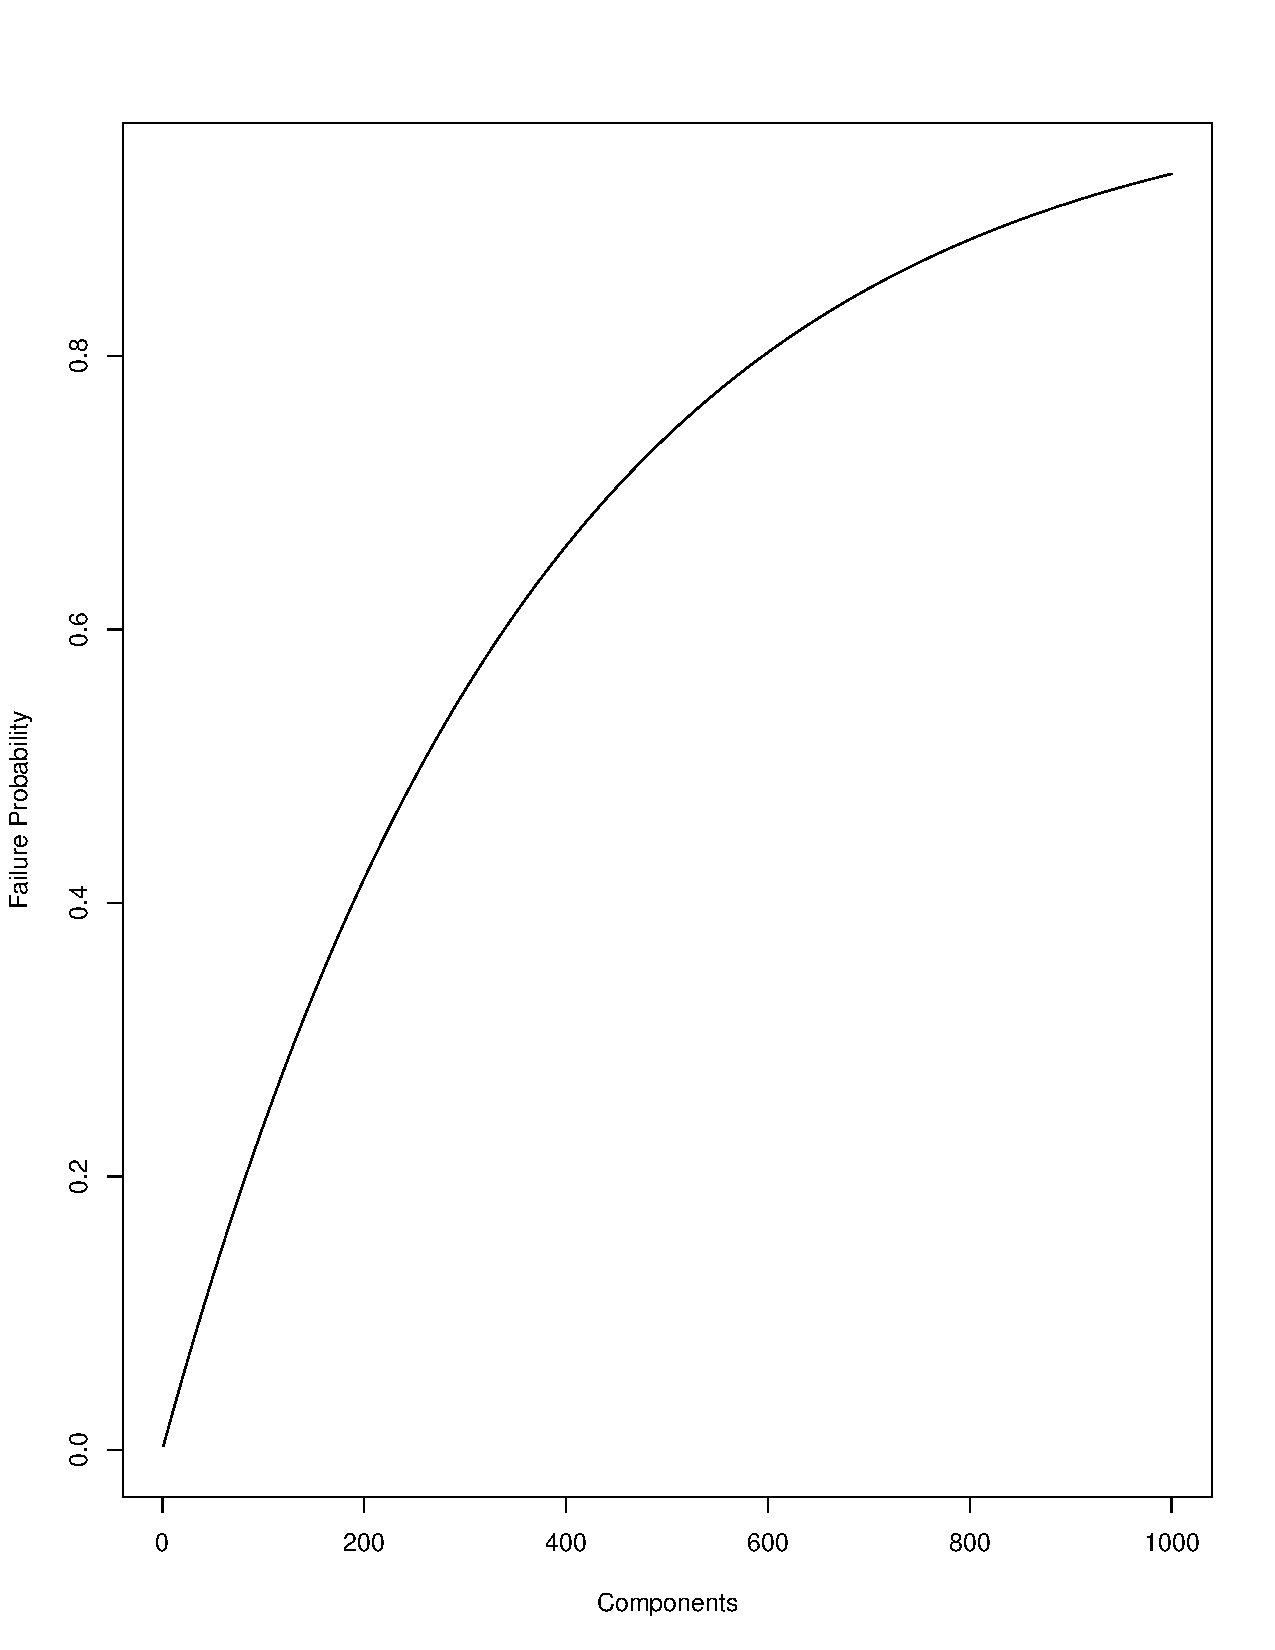
\includegraphics[width=0.8\linewidth]{art/faillure_probability}
\caption[3-sigma probability of failure]{\footnotesize 
	The probability of failure as a function of components under the 3-sigma standard.}
\label{fig:3_sigma_failure_proability}
\end{minipage}\hfill
\begin{minipage}{0.45\textwidth}
\centering
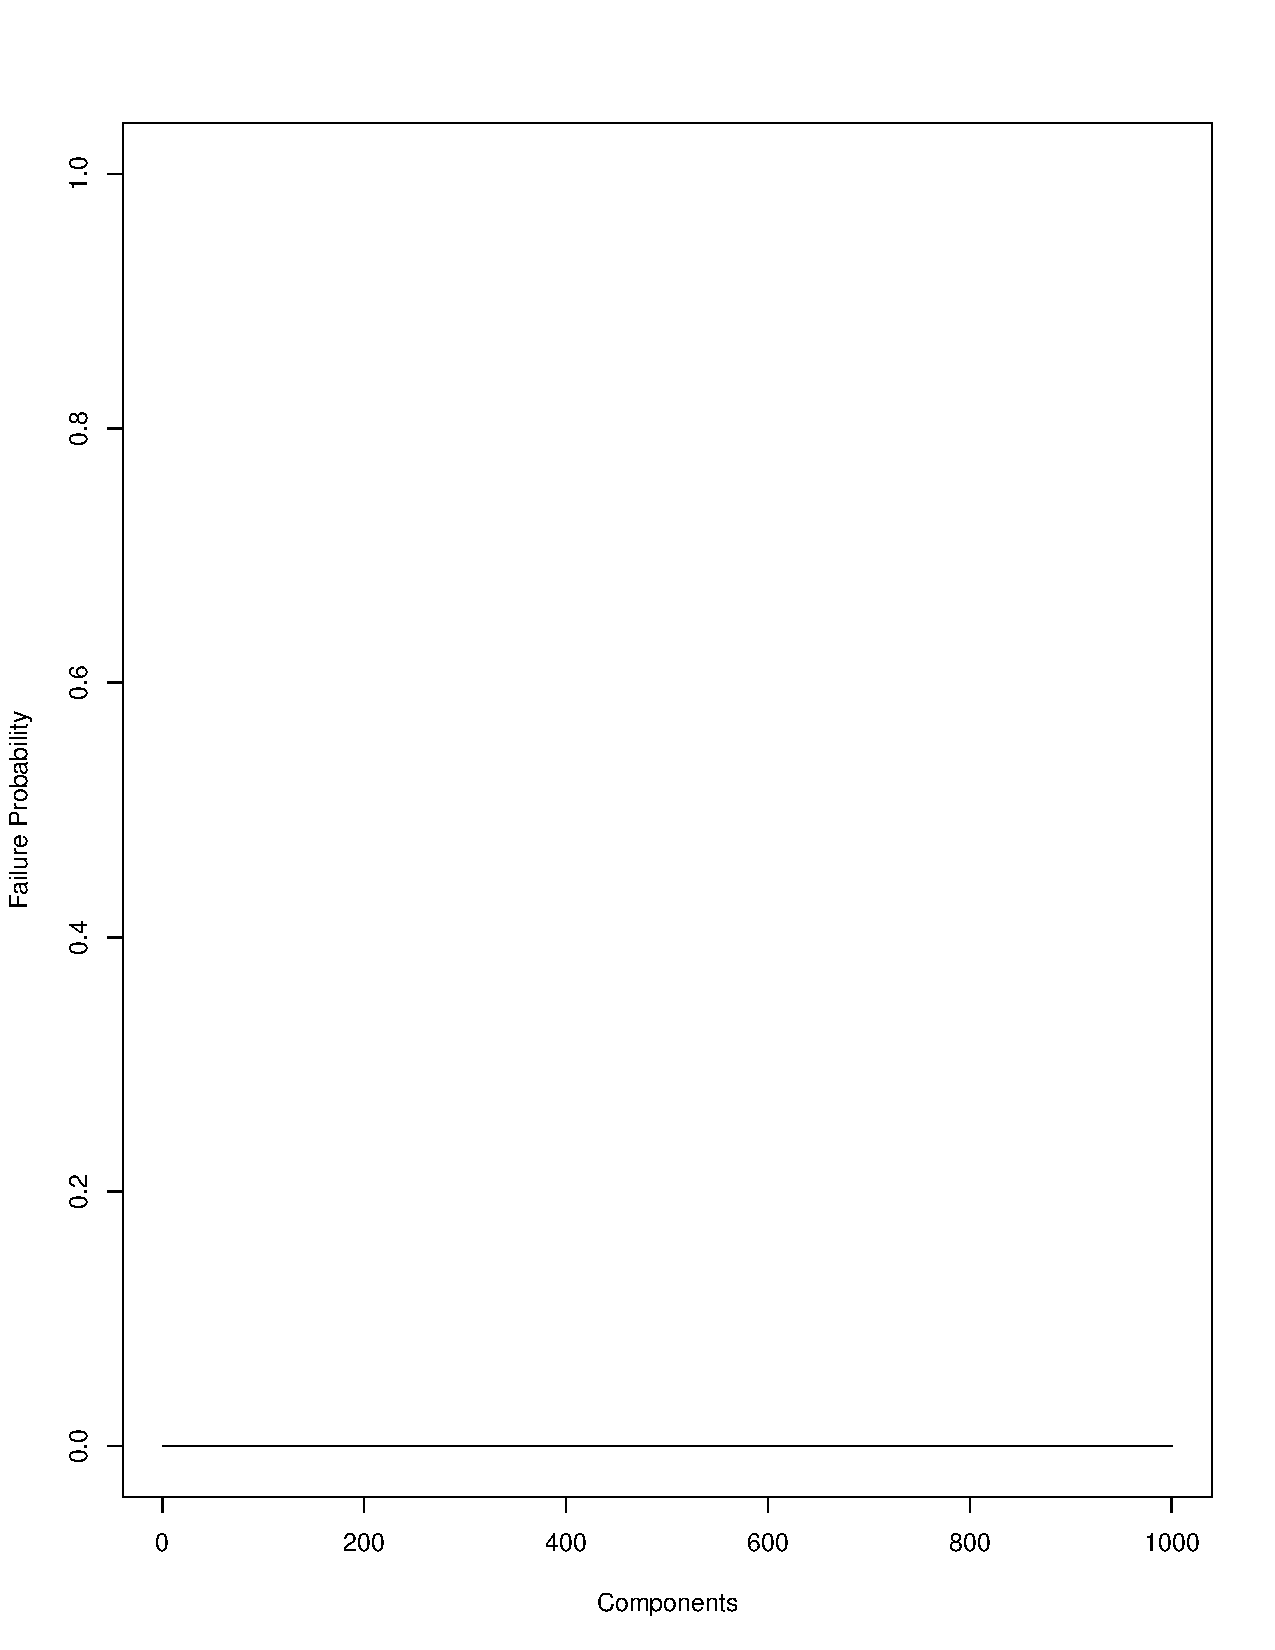
\includegraphics[width=0.8\linewidth]{art/6-sigma_failure_probability}
\caption[6-sigma probability of failure]{\footnotesize 
	The probability of failure as a function of components under the 6-sigma standard.}
\label{fig:6_sigma_failure_proability}
\end{minipage}
\end{figure}

According to \cite{montgomery_introduction_2007}, the 6-sigma methodology has gained more success than it predecessors:
\begin{quote}
The reason for the success of six-sigma in organizations outside the traditional manufacturing sphere is that variability is everywhere, and where there is variability, there is an opportunity to improve business results. 
\end{quote}



\subsection{Lean Systems}
Quoting \cite{wikipedia_lean_2015} (my own emphasis in bold):
\begin{quote}
Essentially, lean is centered on making obvious what \textbf{adds value} by \textbf{reducing everything else}. Lean manufacturing is a management philosophy derived mostly from the Toyota Production System (TPS) (hence the term Toyotism is also prevalent) and identified as ``lean'' only in the 1990s.
\end{quote}

\subsection{Design for Six-Sigma (DFSS)}
\label{sec:dfss}

Quoting \cite{wikipedia_design_2015} (my own emphasis in bold):
\begin{quote}
It is based on the use of \textbf{statistical tools} like linear regression and enables empirical research similar to that performed in other fields, such as social science. While the tools and order used in Six Sigma require a process to be in place and functioning, DFSS has the objective of \textbf{determining the needs of customers} and the business, and driving those needs into the product solution so created. DFSS is relevant for relatively simple items / systems. It is used for product or process design in contrast with process improvement.
\end{quote}




\subsection{Quality Systems and Standards}
The first quality standard was issued by the International Standards Organization (ISO) in $1987$.\marginnote{ISO9000}
Current quality standards are known as the \emph{ISO9000 series}. These include:
\begin{description}
\item [ISO9000:2000] Quality Management System-Fundamentals and Vocabulary.
\item [ISO9001:2000] Quality Management System-Requirements.
\item [ISO9004:2000] Quality Management System-Guidelines for Performance Improvement.
\end{description}
In Israel, it is the Standards Institute of Israel\footnote{\url{https://portal.sii.org.il/heb/qualityauth/certificationtypes/qualitylinks/iso9001/}} that may give ISO9000 (like any ISO) certifications upon inspecting the candidate organization.
As emphasized by \citet[p.24]{montgomery_introduction_2007}, ISO9000 is a set of rules and best practices, mostly oriented at \emph{knowledge management}. 
It may help to \emph{preserve} quality, but it does not, nor does it aim to, \emph{improve} quality.
As such, it will not be the focus of our course, which will focus on \emph{statistical tools}.


\begin{extra}

[TODO: Just-in-Time, Poka-Yoke]

\end{extra}




\section{DMAIC}
There are many names for the process of quantitative re-evaluations of performance against a given target: \emph{data driven decision making} (DDD), \emph{Shewart cycle}, etc.
We will focus on one such framework, illustrated in Figure~\ref{fig:DMAIC} known as DMAIC: Define, Measure, Analyze, Improve, Control.


\begin{figure}[t]
\centering
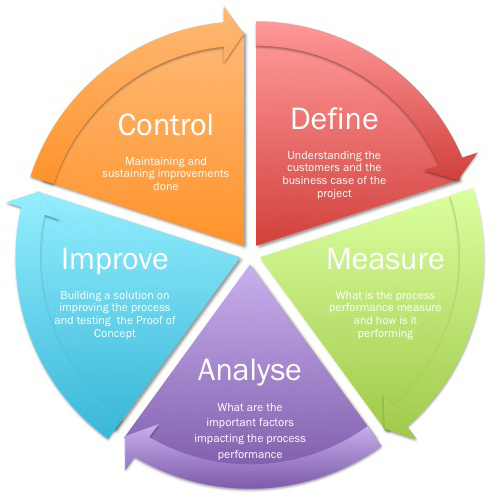
\includegraphics[width=0.6\linewidth]{art/Sigma_detail}
\caption[DMAIC]{The DMAIC cycle. \newline
\url{http://www.sapartners.com/sigma-academy/}}
\label{fig:DMAIC}
\end{figure}

Here are some general observations on DMAIC:
\begin{enumerate}
\item It is aimed at promoting improvement and creative thinking.
\item It is not part of the six-sigma methodology, but will typically take part in its implementation.
\end{enumerate}

What do the stages of DMAIC mean \footnote{\url{http://asq.org/learn-about-quality/six-sigma/overview/dmaic.html}}?
\begin{description}
\item [Define] the problem, improvement activity, opportunity for improvement, the project goals, and customer (internal and external) requirements.
\item [Measure] process performance.
\item [Analyze] the process to determine root causes of variation, poor performance (defects).
\item [Improve] process performance by addressing and eliminating the root causes.
\item [Control] the improved process and future process performance.
\end{description}

In the following chapter we give a set of statistical tools required for \emph{measuring},\emph{analyzing} and \emph{controlling} a process.

% % % % Descriptive Statistics % % % % 
\chapter[EDA]{Exploratory Data Analysis- EDA}
\label{sec:exploratory}


In this chapter, we give a short review of methods for \emph{exploratory data analysis} (EDA), \aka \emph{descriptive statistics}.\marginnote{Descriptive Statistics}
Recall that our goal is an assumptions-free description of our data. 
EDA thus consist of computing interpretable summaries of the data, called \emph{summary statistics}, and visualizations. 


\section{Summary Statistics}
\label{sec:summary_statistics}

We now distinguish between summary statistics that apply to attributes, categorical by definition, and variables, continuous by definition. 


\subsection{Summarizing Categorical Data}

\subsubsection{Univariate}
Summarizing a vector of categorical data can naturally be done by tabulating it, i.e., computing the frequency and relative frequency of each category.
Clearly averages, medians, and the likes are incomputable, since categorical data has no ordering, nor does it admit simple operations such as summation.

\begin{extra}
Variability of categorical data can clearly not be measured by its variance, since it does not admit a summation operation.
It is, however, possible to define different measures of variability that do apply.
The \emph{entropy} is such an example.\marginnote{Entropy}
\end{extra}


\subsubsection{Bivariate}
Generalizing the univariate case to bivariate, or multivariate, one can keep tabulating. I.e., compute the frequency, and relative frequency, of combinations of categories.



\subsection{Summarizing  Continuous Data}
Continuous variables admit many more mathematical manipulations than categorical attributes. 


\subsubsection{Univariate}

We start by presenting the most natural summaries of the data. Without going into the formal definition, we refer to them as \emph{summary of location}.\marginnote{Location Summaries}
These include:

\begin{definition}[The Mean]
The \emph{mean}, or \emph{average}, is defined as 
\begin{align}
	\bar{x}:= \frac{1}{n}\sum_{i=1}^{n} x_i
\end{align}
\end{definition}

\begin{definition}[The Median]
The median is the observation that is smaller than half of the sample and larger than half of the sample.
\end{definition}

\begin{definition}[$\alpha$-Trimmed Mean]
The $\alpha$-trimmed mean is the average of the observations left after ignoring the largest and the smallest $(100\alpha) \%$ of them.
\end{definition}
The \naive average is the $0$-trimmed mean, and the median is the $0.5$-trimmed mean.

From summaries of location, we move to summaries of \emph{scale}. \marginnote{Summary of Scale}

\begin{definition}[The Standard Deviation]
\begin{align}
	s(x):= \sqrt{\frac{1}{n-1} \sum_{i=1}^{n} (x_i-\bar{x})^2}
\end{align}
\end{definition}

For the following, we require the definition of the sample quantiles, themselves \textbf{not} a scale summary.

\begin{definition}[$\alpha$ Quantile]
The $\alpha$-quantile of the sample is the observation that is larger than $(100\alpha)\%$, and smaller then  $(100(1-\alpha))\%$ of the sample. 
\end{definition}
The empirical maximum and minimum are then $x_{1.0}$ and $x_{0.0}$, respectively.


\begin{definition}[The Range]
\begin{align}
	Range(x):= \max_i\set{x_i}-\min_i\set{x_i}= x_{1.0}-x_{0.0}
\end{align}
\end{definition}

\begin{definition}[The Inter Quantile Range- IQR]
\label{def:iqr}
\begin{align}
	IQR(x):= x_{0.75}-x_{0.25}
\end{align}
\end{definition}



\begin{definition}[The Median Absolute Deviation- MAD]
\label{def:mad}
\begin{align}
	MAD(x):= \set{|x_i-x_{0.5}|}_{0.5}
\end{align}
\end{definition}
Note that the MAD may be sometimes scaled by some constant. Particularly in the \R function \rcode{mad()}. 


After summaries of scale, we move to summaries of \emph{skewness}, or \emph{asymmetry}.

\begin{definition}[Yule Skewness Measure]
[TODO: verify]
\begin{align}
	YULE(x):= \frac{(x_{0.75}+x_{0.25})-x_{0.5}}{2 IQR(x)}
\end{align}
\end{definition}

 


\subsubsection{Bivariate}
From univariate data $x$, we move to bivariate $x,y$.
Clearly we can apply univariate summaries component-wise. 
We want, however, to summarize the \emph{joint} behaviour of the data. 
For this purpose, we assume that data comes in pairs, implying that $x$ and $y$ are of same length.
The first measure, is naturally the celebrated (Pearson) correlation coefficient, that captures the level of linear association.


\begin{definition}[(Empirical) Covariance]
\begin{align}
	Cov(x,y):= \frac{\sum_{i=1}^{n} (x_i-\bar{x})(y_i-\bar{y})}{n-1}
\end{align}
\end{definition}



\begin{definition}[Pearson's Correlation Coefficient]
\begin{align}
	r(x,y):= \frac{(n-1) Cov(x,y)}{S(x) S(y)}
\end{align}
\end{definition}
We can dwell into the meaning and intuition underlying Pearson's correlation coefficient, but we will not. 
The curious reader is reffered to \cite{rodgers_thirteen_1988}.

The next measure of association captures a more general association.
\begin{definition}[Spearman's Correlation Coefficient]
Spearman's correlation coefficient is merely Pearson's correlation coefficient computed on the \emph{ranks} of $x$ and $y$. 
\end{definition}

We conclude by noting that \emph{regression coefficients} are also a measure of association. 





\subsubsection{Multivariate Data}
Multivariate data, both continuous (variables), and discrete (attributes), admits a vast realm of method for summary and visualization.
Clearly, associations between several variables can be very complicated so that the more we try to summarize, the more information we give up. On the other hand, and unlike the univariate and bivariate case, our minds will need some type of simplification since they cannot grasp the raw data (did you ever try to imagine how $\mathbb{R}^4$ looks like?).
As usual, we emphasize that our purpose is to summarize the joint association in the data. 
For component-wise summaries, we can always apply the univariate summaries one variable at a time. 

By far the most popular measures of joint association are the covariance matrix and correlation matrix.

\begin{definition}[Covariance Matrix]
For a multivariate data consisting of $x_1,\dots,x_p$ vectors, each with $n$ entries: $x_{i,1},\dots,x_{i,n}$, we define the (sample) covariance matrix to be a $p\times p$ matrix whose elements are the (sample) covariances between corresponding vectors:
\begin{align}
	\hat{\Sigma}_{i,j}:= Cov(x_i, x_j)
\end{align}
\end{definition}


\begin{extra}[Sample Covariance Matrix]
The matrix $\hat{\Sigma}$ has many useful properties. 
The curious reader is referred to \cite{petersen_matrix_2006}, and references therein, for more details.
\end{extra}

\begin{definition}[Correlation Matrix]
For a multivariate data consisting of $x_1,\dots,x_p$ vectors, each with $n$ entries: $x_{j,1},\dots,x_{j,n}$, we define the (sample) correlation matrix to be a $p\times p$ matrix whose elements are the (Pearson) correlations between corresponding vectors:
\begin{align}
	\hat{R}_{i,j}:= r(x_i, x_j)
\end{align}
\end{definition}


\begin{extra}[Multivariate Data Analysis]
Multivariate analysis is an important, and very actively studied field in statistics and machine learning.
A non-comprehensive list of methods that belong to this realm include 
Principal Component Analysis (PCA),\marginnote{PCA, SVD,ICA}
Singular Value Decomposition (SVD), 
Factor Analysis (FA), 
Independent Component Analysis (ICA),
Dimensionality Reduction, 
Manifold Learning, 
Self Organizing Maps, 
etc.
Ask me for reference books or courses if this topic interests you.
\end{extra}

\afterpage{\clearpage}


\section{Visualization}
\label{sec:visualizations}

\subsection{Visualizing Categorical Data}



\subsubsection{Univariate}
Much like computing summaries, there is not much to be said about visualizing univariate categorical variables. 
The most natural, and perhaps only visualization, is the \emph{bar plot}, illustrated in Figure~\ref{fig:barplot}.



\begin{figure}[h]
\centering
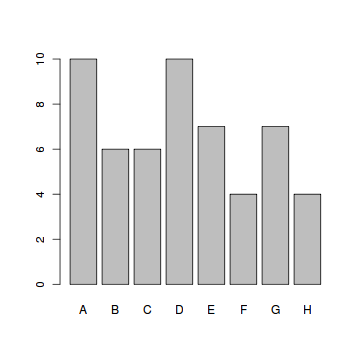
\includegraphics[height=0.3\textheight]{art/categorical-data1x}
\caption[Bar Plot]{The Bar-Plot. \newline
\url{http://www.r-tutor.com/elementary-statistics/qualitative-data/bar-graph}}
\label{fig:barplot}
\end{figure}



\subsubsection{Bivariate}
Visualizing a two-way cross-table can be done using an extension of the bar-plot.
Several extensions exist. By far, the most informative and recommended figure, in this author's view, is the \emph{mosaic plot}, illustrated in Figure~\ref{fig:mosaic}. \marginnote{Mosaic Plot}

\begin{figure}[h]
\centering
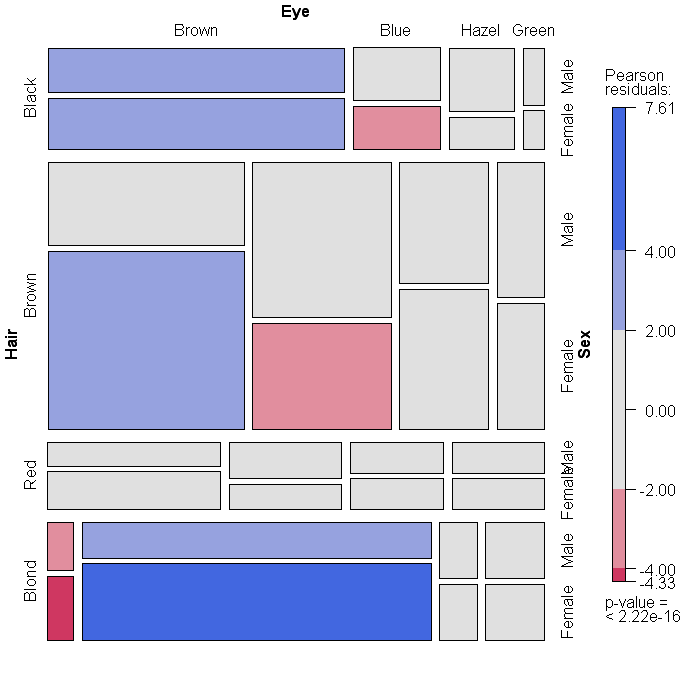
\includegraphics[height=0.3\textheight]{art/mosaic1}
\caption[Mosaic Plot]{Mosaic Plot. \newline
\url{http://www.statmethods.net/advgraphs/mosaic.html}}
\label{fig:mosaic}
\end{figure}







\afterpage{\clearpage}


\subsection{Visualizing Continuous Data}




\subsubsection{Univariate}
Visualization of univariate continuous vectors can present the raw data, or it distribution (i.e.- discarding the indexes).
The most basic visualizations are the \emph{dotchart}, \emph{histogram}, \emph{boxplot}, \emph{stem-and-leaf plot}. 
These are illustrated in figures \ref{fig:dot_plot}, \ref{fig:histogram_eruptions}, \ref{fig:boxplot}, \ref{fig:stem_and_leaf} respectively. 


 
\begin{figure}[h]
\centering
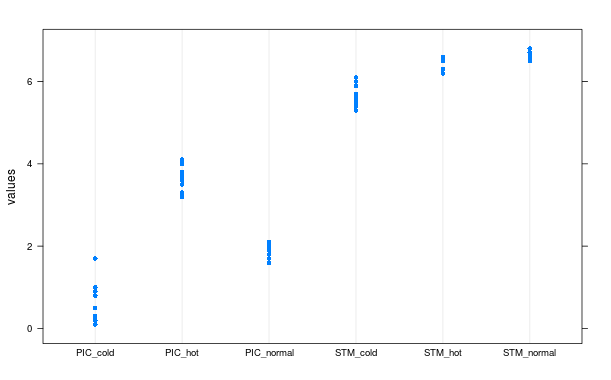
\includegraphics[height=0.3\textheight]{art/lmCm0}
\caption[Dot Plot]{Dot Plot. \newline \url{http://stackoverflow.com/questions/15109822/r-creating-scatter-plot-from-data-frame}}
\label{fig:dot_plot}
\end{figure}



\begin{figure}[h]
\centering
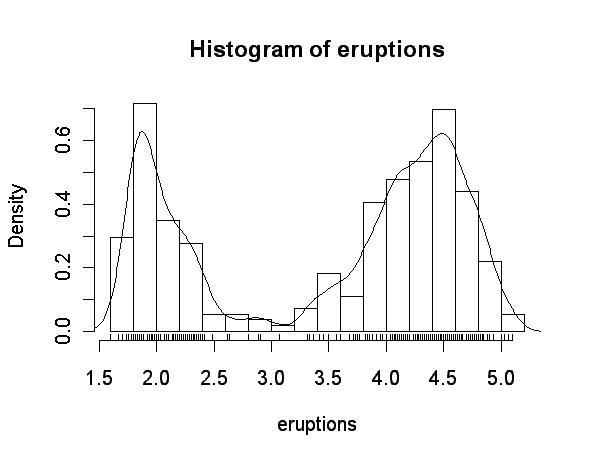
\includegraphics[height=0.3\textheight]{art/histogram_eruptions}
\caption[Histogram]{Histogram. \newline
\url{http://compbio.pbworks.com/w/page/16252882/Basic}}
\label{fig:histogram_eruptions}
\end{figure}

\begin{figure}[h]
\centering
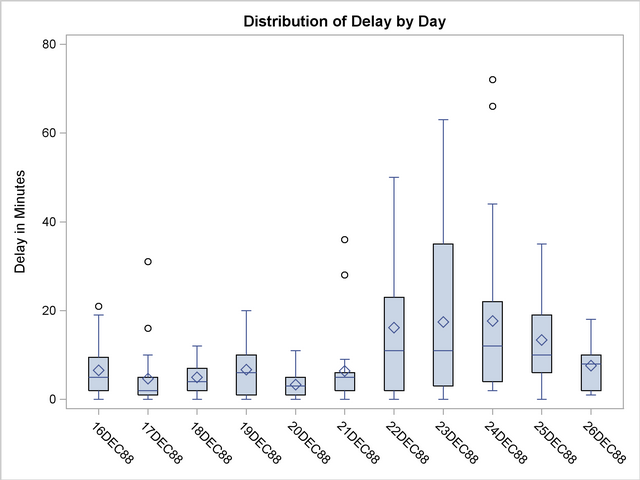
\includegraphics[height=0.3\textheight]{art/ex6aout}
\caption[BoxPlot]{Boxplot. \newline \url{http://support.sas.com/documentation/cdl/en/statug/63033/HTML/default/viewer.htm}}
\label{fig:boxplot}
\end{figure}



\begin{figure}[h]
\centering
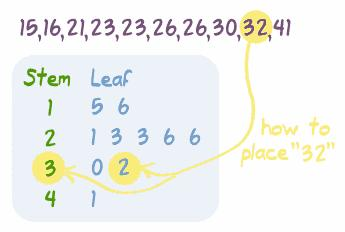
\includegraphics[height=0.3\textheight]{art/stem_and_leaf}
\caption[Stem and Leaf Pot]{Stem-and-leaf plot. \newline
\url{https://www.mathsisfun.com/data/stem-leaf-plots.html}}
\label{fig:stem_and_leaf}
\end{figure}




\subsubsection{Bivariate}
The simultaneous visualization of two continuous variables, can naturally be done with a \emph{scatter plot}.
More sophisticated visualization, which generalizes the histogram into two dimensions, is the \emph{hexbin plot}.  
These are illustrated in figures \ref{fig:scatterplot}, and \ref{fig:hexbin}, respectively. 


\begin{figure}[h]
\centering
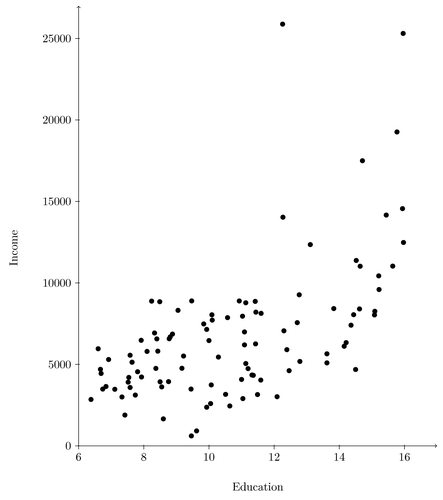
\includegraphics[height=0.3\textheight]{art/scatterplot}
\caption[Scatter Plot]{Scatter Plot. \newline 
\url{http://texample.net/tikz/examples/scatterplot/}}
\label{fig:scatterplot}
\end{figure}





\begin{figure}[h]
\centering
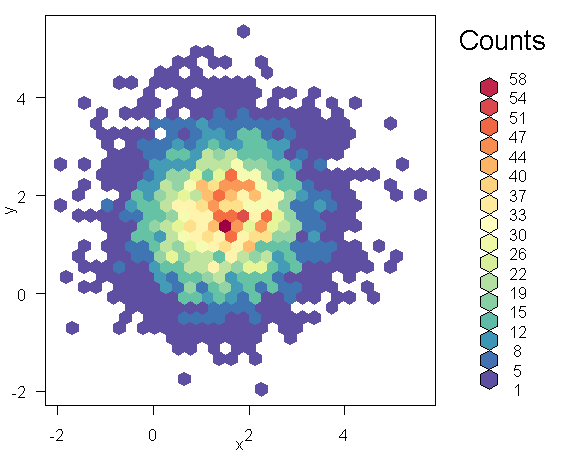
\includegraphics[height=0.3\textheight]{art/hexbin2}
\caption[HexBin Plot]{HexBin plot. Sorce: \url{http://www.r-bloggers.com/5-ways-to-do-2d-histograms-in-r/}}
\label{fig:hexbin}
\end{figure}






\subsubsection{Multivariate Data}
Since we cannot possibly visualize data in more than $3$-dimensions, and we clearly prefer data in $1$ or $2$ dimensions, the visualization of multivariate data will typically consist of summarizing the data into $1D$ or $2D$, and then applying the above mentioned visualization techniques.

An important exception is due to the observation that a computer image, is essentially a matrix. 
We can thus visualize matrices, with a simple image, and in particular, covariance and correlation matrices, as illustrated in Figure~\ref{fig:covariance_image}.

A second exception is when the data has both continous variables and discrete attributes. 
Endlessly many combinations are then possible.
The author strongly recommends to visit Hans Rosling's \emph{Gap Minder} at \url{http://www.gapminder.org/world} for an excellent interactive visualization. \marginnote{Gap Minder}


\begin{figure}[h]
\centering
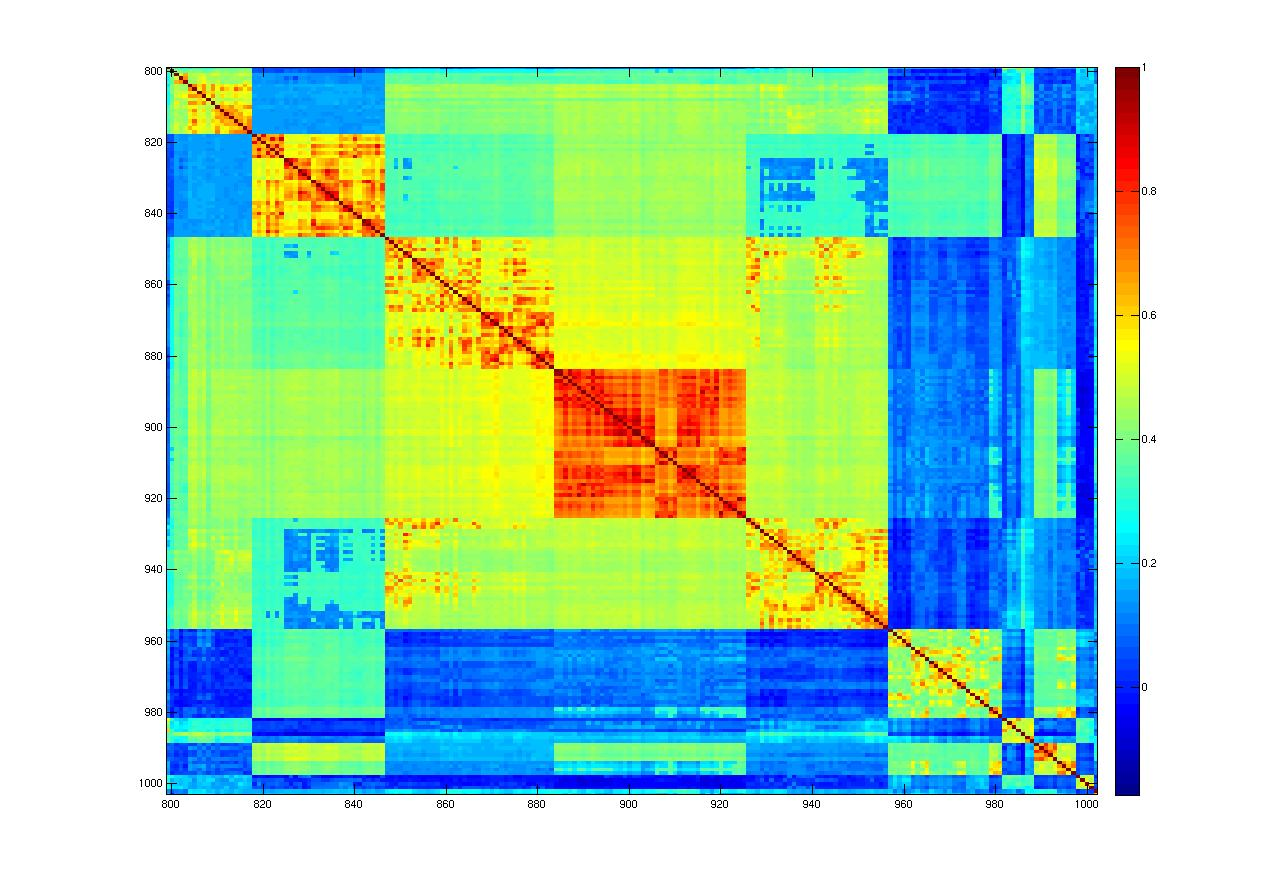
\includegraphics[height=0.3\textheight]{art/covarianceSupervised}
\caption[Covariance Matrix]{Image of covariance matrix. \newline
\url{http://cs.brown.edu/courses/csci1950-g/results/final/sghosh/}}
\label{fig:covariance_image}
\end{figure}




\subsection{On-Line Visualization}
For the purpose of quality control, we may often want an \emph{on-line} visualization, and not \emph{off-line}, as the ones previously discussed.
This is the purpose of \emph{dashboards}, illustrated in Figure~\ref{fig:dashboard}.\marginnote{Dashboard}

\begin{figure}[h]
\centering
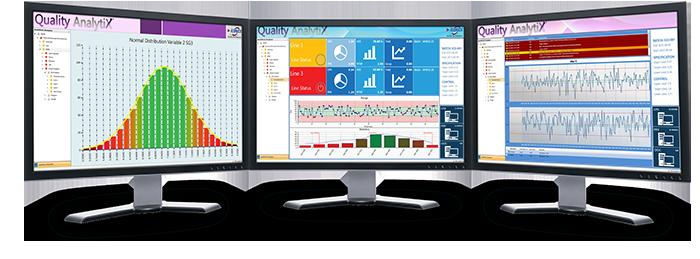
\includegraphics[height=0.3\textheight, width=0.9\linewidth]{art/dashboard}
\caption[Dashboard]{Dashboard. \newline
\url{http://www.iconics.com/Home/Products/AnalytiX/Quality-AnalytiX.aspx}}
\label{fig:dashboard}
\end{figure}

\afterpage{\clearpage}


% % % % Statistical inference % % % %
\chapter{Statistical Inference} 
\chaptermark{Inference}
\label{sec:inference}

The idea of extrapolating knowledge from a \emph{sample} to a population is known as \emph{statistical inference}.
It encompasses the ideas of \emph{parameter estimation}, \emph{confidence intervals}, and \emph{hypothesis testing}.
We will assume the reader is familiar with these, but recall some required terminology.
The QC and SPC terminology are not always consistent with statisticians' terminology. When new names are given to old ideas, we will emphasize this in the text.

\begin{description}
\item [Null/Alternative Hypothesis] Some statement about the world we wish to test with data. The frequentist argument follows a Popperian philosophy\footnote{Following Karl Popper's philosophy of science, we can never know that something is true, we can only know when it is not true. Popper philosophy was motivated by the fact that no one suspected Isaac Newton's mechanics to be wrong, until relativity theory was proposed by Einstein.}: to show the alternative hypothesis is true, we will show that the null hypothesis is not true. 
In the context of quality control, the null hypothesis will be the process is \emph{in statistical control}, while the alternative will be that it is \emph{out of control}.\marginnote{In Control}
Other terms for the alternative hypothesis are the \emph{research hypothesis}, or simply the \emph{signal}.
\item [Statistical Test] The procedure of inferring from data on the truthfulness of the alternative hypothesis.
\item [Assumptions] As the name suggests, these are assumptions. We stress that unlike hypothesis, assumptions are not being tested in a statistical test. 
\item [Test Statistic] The function of the data to be computed for the purpose of inference. As such, it is a random variable. 
May also be though of as a \emph{signal detector}.
\item [Null/Alternative Distribution] The distribution of the test statistic under the null/alternative hypothesis.
\item [Type I/II error] See Figure~\ref{fig:confusion_table}.
\item [False/True Positive/Negative] See Figure~\ref{fig:confusion_table}.
\item [Rejection Region] The collection of event that will lead us to reject the null hypothesis, and believe in the alternative hypothesis.
\item [p-value] A.k.a. \emph{observed significance}. The null probability of the observed (or ``more extreme'') event.
\item [Significance Level] A.k.a. $\alpha$. The probability of a false positive.
\item [Power] The probability of a true positive.
\item [i.i.d.] ``Independent and identically distributed'' (i.i.d.) is an assumption made on the sampling distribution, meaning that samples are statistically independent, and all originating from the same distribution.

\end{description}

\begin{figure}
\centering
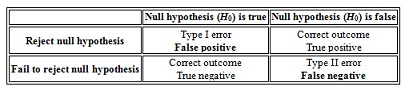
\includegraphics[width=0.8\linewidth]{art/Beware-of-False-Positives-Chart-1}
\caption[Confusion Table]{Type I/II error confusion table. \newline \url{https://infocus.emc.com/william_schmarzo/beware-of-false-positives/}}
\label{fig:confusion_table}
\end{figure}


\begin{extra}[ROC termininology]
%TODO: ROC terminology

The engineering, statistical, and information retrieval literature, define error and precision criteria\footnote{\url{https://en.wikipedia.org/wiki/Receiver_operating_characteristic}}:
\begin{description}
	\item[True Positive Rate] ...
	\item[Sensitivity] ...
	\item[Recall] ...
	\item[False Positive Rate] ...
	\item[Fallout] ...
	\item[Specificity]
	\item[Miss Rate]
	\item[Prevalence]
	\item[True Negative Rate]
	\item[Accuracy]
	\item[Positive Predictive Value]
	\item[Precision] 
	\item[False Omission rate]
	\item[False Discovery Rate]
	\item[Negative Predictive Value]
	\item[Positive Likelihood Ratio]
	\item[Negative Likelihood ratio]
	\item[Disgnostic odds ratio]
\end{description}
\end{extra}


The following sections of this chapter present particular statistical inference methods we will be using in the following chapters.


\begin{think}
Can you design a test with type I error larger its power?
Would you ever want such a test?
Think about it using the analogy to statistical tests and criminal courts. 
\end{think}




% % % Capabilty Analysis
\chapter[Capability]{System Capability Analysis}
\label{sec:capability_analysis}

In a \emph{system capability analysis}, we essentially use statistical tools to measure the variability in a production process.
This analysis can answer questions that are raised at the measuring, analyzing, and improving stages of the DMAIC cycle. 
The methods we will discus compare between the processes variability and its specifications. 
Note, however, that a simple statistical analysis of the production process, without relating to specification, may also qualify as a system capability analysis.

We naturally want production processes that adhere to specifications, and want to quantify the level of adherence.
The quantification is performed by comparing the variability in a CTQ to the specification.
In this chapter we assume the process’s capability is fixed over time. 
In Chapter~\ref{sec:advanced_capability_analysis} we revisit the same problems, when allowing the process’s capability to vary over time. 

The particular setup discussed in this chapter is also known as \emph{product specification}.\marginnote{Product Specification}
When we use the actual time, and ordering of data samples, as in a control chart, we will no longer regard it as product specification but rather as a bona-fide capability analysis. This is the subject of Chapter~\ref{sec:advanced_capability_analysis}.



 
 
 
Because capability analysis, or product specification, is essentially the study of the CTQ's distribution, it can be approached with the aforementioned statistical tools such as univariate summary statistics and visualizations presented in Sections~\ref{sec:summary_statistics} and \ref{sec:visualizations}.
To test a particular hypothesis want to be tested on the distribution of the CTQ, we may call upon the inference tools from Chapter~\ref{sec:inference}.




\section[PCRs]{Process Capacity Indexes}
Classical statistical devices do not incorporate the designed process's capabilities.
\emph{Process capability ratios} (PCR), or \emph{process capability indexes}, are merely population parameters that also depend on specifications.\marginnote{Process Capability Index}
The first, and most basic PCR is the $\cp$ of a particular CTQ.

\begin{definition}[$\cp$]
\begin{align}
\label{eq:cp}
	C_p:= \frac{USL-LSL}{6 \sigma}, 
\end{align}
where $\sigma$ is the standard deviation of the CTQ.

\end{definition}
Clearly $\cp$ is a process parameter, that needs to be estimated.
\begin{definition}[$\cpHat$]
\begin{align}
	\cpHat:= \frac{USL-LSL}{6 \hat{\sigma}}, 
\end{align}
where $\hat{\sigma}$ is some estimate of the standard deviation of the CTQ.
\end{definition}
The most natural $\hat{\sigma}$ is the sample standard deviation $s$, but we will explore other options in the following.


There is a relation between $C_p$ and the probability of non-conformance. 
To explore this relation we introduce the following notation:
\begin{tcolorbox}
\footnotesize
\textbf{Collecting Notation} \newline
$\targetValue:= (USL+LSL)/2$, the target value. \newline
$\delta:= (USL-LSL)/2$, the specification tolerance. $USL=\targetValue+\delta, LSL=\targetValue-\delta$.  \newline
$\ctqExpect:= \expect{CTQ}$, the expected CTQ. \newline
$\pnc:= 1-P(CTQ \in [LSL,USL])$, the probability of non compliance. 
\end{tcolorbox}

With our new notation Eq.(\ref{eq:cp}) is now $\cp=\frac{\delta}{3 \sigma}$.
Assuming $CTQ \sim \gauss{\mu, \sigma^2}$, and that the process is centred so that $\ctqExpect=\targetValue$, then $\cp$ is related to $\pnc$ via
\begin{align}
\label{eq:pc_and_pnc}
	\pnc= 2\, \Phi(-3 \cp)
\end{align}
As a sanity check, we check this relation for a 3-sigma process.
A 3-sigma process implies that $\cp=1$, and Eq.(\ref{eq:pc_and_pnc}) returns $\pnc=0.0027$, as we have already seen in the introduction (Section~\ref{sec:six_sigma}).

\cite{montgomery_introduction_2007} recommends the following $\cp$ values:

\begin{tabular}{|c|c|c|}
\hline  & $\cp$ Value & Implied ppm \\ 
\hline \hline Existing processes
 & 1.33
 & 66 \\ 
\hline New processes
 & 1.50
 & 6.8 \\ 
\hline Safety, strength, or critical
parameter, existing process
 & 1.50
 & 6.8 \\ 
\hline Safety, strength, or critical
parameter, new process
 & 1.67
 & 0.5 \\ 
\hline Six Sigma quality process & 2.00 &  0.002 \\ 
\hline 
\end{tabular} 

\bigskip

To derive Eq.(\ref{eq:pc_and_pnc}), and thus the ppm column in the table, we had to call upon several assumptions.
Namely:
\begin{enumerate}
\item The process is in statistical control, i.e. $\ctqExpect$ is fixed over time
\item The CTQ has a normal distribution.
\item The process is centred, i.e. $\ctqExpect=\targetValue$.
\item $\targetValue$ is mid-way between LSL and USL.
\end{enumerate}








\subsection{Non-Conformance for a Non-Gaussian CTQ}
The first assumption we will now relax is the Gaussianity of $CTQ$. 
We start by checking what is the fallout rate, if we were completely wrong about the distribution of the CTQ. 
Chebyshev's inequality provides a universal bound on $\pnc$ for a $\cp=1$ process.


\begin{theorem}[Chebyshev's inequality]
For any random variable $\x$, with $\mu:=\expect{\x}$, and $\sigma^2:=\expect{(\x-\mu)^2}$, then
\begin{align}
	P(|\x-\mu| \geq k\sigma) \leq \frac{1}{k^2}
\end{align}
\end{theorem}
If $\cp=1$  then $\delta=3\sigma$. Plugging $k=3$ in the inequality returns $\pnc<0.11$.
This means that a 3-sigma process, assumingly with $2,700 ppm$, may actually have $111,111 ppm$, if we were wrong about the Gaussianity assumption.


%\begin{theorem}[Vysochanskij–Petunin inequality]
%For any random variable $\x$, with $\mu:=\expect{\x}$, $\sigma^2:=\expect{(\x-\mu)^2}$, with unimodal distribution, and for $k>\sqrt{8/3}=1.63299$, then 
%\begin{align}
%	P(|\x-\mu|>k\sigma)=\frac{4}{9 k^2}
%\end{align}
%\end{theorem}
%Since $3$ is obviously larger than $1.63299$, then an immediate application of Vysochanskij–Petunin inequality yields that for a unimodal CTQ, then $\pnc<0.0493$, or $49,383 ppm$.
%
%
%
%
%
%Can we tighten the bound on $\alpha$ by adopting some other weak assumption?
%Certainly!
%We can use the fact that 
%If we are willing to assume that the production process is such that the CTQ of two consecutive units will never be larger than some $c$: 
%\begin{align}
%\label{eq:bounded_rv}
%	P(|x_{i,t}-x_{i-1,t}|<c)=1.
%\end{align}
%\begin{theorem}[Azuma-Hoeffding Inequality]
%For an arbitrary sampling process for which Eq.(\ref{eq:bounded_rv}) holds, then 
%\begin{align}
%	P(|\bar{x}_t-\ctqExpect| \geq s ) \leq  2 \exp \left( -\frac{n s^2 }{2c^2} \right)
%\end{align}
%\end{theorem}
%
%
%
%Again we see that if we wrongly assumed normality, we may have many more non-compliances than we thought. Then again, both Chebyshev and Vysochanskij–Petunin are very loose bounds. 
%They should thus be seen as a worst-case, while reality is not as bad.

The moral of the story is that by assuming the correct distribution of the CTQ, we may save a lot of resources. 
We can assume normality, as we typically do, but there are other alternatives:
\begin{enumerate}
\item Transformations: it is quite possible that the CTQ is not Gaussian in its original scale, but it is Gaussian in a different scale. You should always inspect a QQnorm (Sec. \ref{sec:qqplot}) plot after a $log$ or $sqrt$ transformation.
\item Assume a different distribution: We derived $\pnc(\cp)$ (eq.~\ref{eq:pc_and_pnc}) under a normality assumption, but it may certainly be derived for different distributions. 
\item The denominator of $\cp$ is a range that leaves $0.00135$ probability of the Gaussian tail outside the range. 
When relaxing the normality assumption, $\sigma$ is no longer related to the tail probability as it was before. We may still, however, directly plug $CTQ_{0.00135}$ and $CTQ_{1-0.00135}$ quantiles to get a CPR in the same spirit of the $\cp$. This is known as the $\cpq$ index we now define.
\end{enumerate}

\begin{definition}[$\cpq$]
\begin{align}
	\cpq:= \frac{USL-LSL}{CTQ_{1-0.00135}-CTQ_{0.00135}}
\end{align}
\end{definition}






\subsection{Process Capability of a Non-Centred Process}
We will now relax the assumption of $\ctqExpect=\targetValue$, while still in statistical control.

\begin{definition}[$\cpk$]
\begin{align}
	\cpk:= \min\set{\cpu,\cpl}
\end{align}
where $\cpu:= \frac{USL- \ctqExpect}{3 \sigma}$ and $\cpl:= \frac{\ctqExpect-LSL}{3 \sigma}$.
\end{definition}
For a non-centred process, this definition is more informative on the probability of non-compliance.
Indeed, Eq.(\ref{eq:pc_and_pnc}) will not hold, but we can derive an updated version:
\begin{align}
	 \pnc \approx \Phi(-3 \cpk).
\end{align}
Generally, $\cpk \leq \cp$, with equality holding for centred processes ($\ctqExpect=\targetValue$).
An illustration is given in Figure~\ref{fig:cpk}.


\begin{figure}
\centering
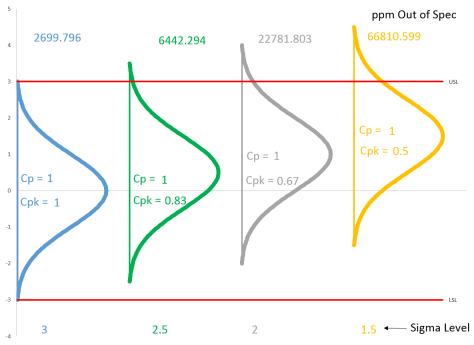
\includegraphics[height=0.3\textheight]{art/Cpk_same_sigma_varying_avg}
\caption[$\cpk$ and $\cp$]{$\cpk$ and $\cp$. \newline
\url{https://www.spcforexcel.com/knowledge/process-capability/interactive-look-process-capability}.}
\label{fig:cpk}
\end{figure}



The $\cpk$ index is motivated by conserving the relation between the index and the fallout rate $\pnc$, which is not captured by $\cp$ when the process is not centred. 
Another index, known as $\cpm$, or the \emph{Taguchi capability index}, also deals with the non centring but slightly differently. It is motivated by the observation that for $\ctqExpect=\targetValue$, then $\sigma=\sqrt{\expect{(CTQ-\targetValue)^2}}$. This relation does not hold if $\ctqExpect \not=\targetValue$, which leads us to the following definition:
\begin{definition}[$\cpm$]
\begin{align}
		\cpm &:= \frac{USL-LSL}{6 \sqrt{\expect{(CTQ-\targetValue)^2}}} \\
		&= 	\frac{USL-LSL}{6 \sqrt{\sigma^2+(\ctqExpect-\targetValue)^2}} \\ 
		&= \frac{\cp}{\sqrt{1+(\frac{\ctqExpect-\targetValue}{\sigma})^2}}. \label{eq:cpm}
\end{align}
\end{definition}
Eq.(\ref{eq:cpm}) readily shows that just like the $\cpk$, then $\cpm \leq \cp$. 








\subsection{Interval Estimation for Capability Indexes}
Since the various process capability indexes are merely population parameters, we can also construct confidence intervals (CIs) for them, which may be very informative if sample sizes are small.
The simplest case is that of $\cp$. Being a monotone transformation of $\sigma$, we can call upon confidence intervals for the variance of a normal population, so that with probability $1-\alpha$:
\begin{align}
\label{eq:ci_for_cp}
	\cp \in \left[ 
		\cpHat \sqrt{\frac{\chi^2_{\alpha/2,n-1}}{n-1}},
		\cpHat \sqrt{\frac{\chi^2_{1-\alpha/2,n-1}}{n-1}}
	\right].
\end{align}
This equation is simply derived from Eq.(\ref{eq:cp_dist}).
Intervals for the other capability indexes, are available in \cite{montgomery_introduction_2007} and references therein. 




\subsection{Testing Hypotheses on Capability}
Consider a supply contract, which requires production to have $\cp>1.5$. 
It may easily be the case, that the $\cp>1.5$, even if $\cpHat<1.5$, especially if the sample size is small.
It thus makes a lot of sense, to design hypothesis tests on process capabilities. 
We observe that for an i.i.d. sample from a Gaussian population, where $\cpHat$ is estimated with $s$, then
\begin{align}
\label{eq:cp_dist}
	(n-1) \left( \frac{\cp}{\cpHat} \right)^2  \sim \chi^2_{n-1}
\end{align} 
so that $(n-1) \left( \frac{\cp}{\cpHat} \right)^2 $ may serve as test statistic.

\begin{example}[$\cp$ test for 6-sigma compliance]
\begin{align*}
	H_0: \cp &\leq 2	\\
	H_1:\cp &> 2 \\
	(n-1) \left( \frac{2}{\cpHat} \right)^2  &\overset{H_0}{\sim} \chi^2_{n-1}
\end{align*}
so that the $1-\alpha$ rejection region in $\cpHat$ scale is 
\begin{align*}
	\cpHat > \sqrt{\frac{4 (n-1)}{\chi^2_{n-1,\alpha}}} .
\end{align*}
\end{example}
Note that we should not be testing this hypothesis with the confidence interval in Eq.(\ref{eq:ci_for_cp}) because this particular hypothesis is directional.
Now for a more general case:
\begin{align*}
	H_0: \cp \leq a; 
	H_1:\cp > a 
	&\Rightarrow \text{reject if } \cpHat > \sqrt{\frac{a^2 (n-1)}{\chi^2_{n-1,\alpha}}},\\
	H_0: \cp \geq  a; 
	H_1:\cp < a 
	&\Rightarrow \text{reject if } \cpHat < \sqrt{\frac{a^2 (n-1)}{\chi^2_{n-1,1-\alpha}}}, \\
	H_0: \cp =  a; 
	H_1:\cp \neq a 
	&\Rightarrow \text{reject if } \cpHat < \sqrt{\frac{a^2 (n-1)}{\chi^2_{n-1,1-\alpha/2}}}
	\text{ or } \cpHat > \sqrt{\frac{a^2 (n-1)}{\chi^2_{n-1,\alpha/2}}} \\
\end{align*}






\subsection{In Practice}
By this point in our discussion you should have noted that to understand a capability index, we always revert to the probability of non compliance, particularly of a 3-sigma process.
Is may not surprise you then, that perhaps the most frequently used capability indexes are simply the probability of non compliance, $\pnc$, and the ``sigma level''.
By sigma-level, we mean $\frac{USL-LSL}{2\sigma}=\frac{\delta}{\sigma}$. 









\subsection{Process Performance Indices}
Process \emph{performance} indices measure compliance to specification of a process out of statistical control. 
These include the $\pp$ and $\ppk$ indices. 
Besides mentioning their existence, we will not give them further attention, since we adopt \cite{montgomery_introduction_2007}'s view that their use is strongly discouraged. 


\begin{remark}
At this point, I hope you are wondering why isn't the fallout rate, $\pnc$, not used as a capability index. 
Well, it is this author's view, that is it probably the best index of them all.
\end{remark}



% % % % SPC
\chapter{Statistical Process Control- SPC}
\label{sec:spc}

Statistical process control, \aka \emph{change detection algorithms} deals with the quantitative analysis of a ``process'', which may be a production line, a service, or any other repeated operation.\marginnote{Change Detection}
As such, it may be found in the Analyze, Improve, and Control stages of the DMAIC cycle.
The purpose of the SPC, in the terms coined by Shewart, is to seperate the variability in the process into \emph{assignable} causes of variation and \emph{chance} causes of variation.\marginnote{Causes of variation}
These are also known as \emph{special} and \emph{common} causes of variation, respectively. 
A process is said to be in \emph{statistical control} if all its variation is attributable to chance causes.
If this is not the case, we call it \emph{out of control} and we will seek the assignable causes, remove then, and   re-analyze.


All the previously mentioned statistical tools may be called upon for this analysis. 
In the context of process control, a subset of tools has gained the nick-name ``The Magnificent Seven''. These include:
\begin{description}
\item Histogram and stem-and-leaf plot. As described in Chapter~\ref{sec:exploratory}.
\item Check Sheet. [TODO: add figure]
\item Pareto chart. An ordered bar plot of the events due to the various assignable variability causes. [TODO: add figure]
\item Cause-and-effect diagram. A visualization of candidate assignable variability causes. [TODO: add figure]
\item Defect concentration diagram. A visual inspection of the location of defects on the product. 
\item Scatter plot. As described in Chapter~\ref{sec:exploratory}.
\item Control chart. A powerful analysis tool to which we devote the rest of this chapter. 
\end{description}





%\begin{pgfpicture}
%    \pgftext{\pgfimage[width=0.6\linewidth, height=0.3\textheight]{}}
%\end{pgfpicture}



\begin{extra}[A more rigorous treatment ]
The contents of this chapter is mostly derived from \cite{montgomery_introduction_2007}. 
For a more mathematically rigorous treatment of the topic see \cite{basseville_detection_1993}.
For an \R oriented exposition of the topic, see \cite{qiu_introduction_2013}.
\end{extra}

\section{A soft start. The \barxChart}


% basic idea
% descion variables: sample size, intervals, statistic, limits, rational groupins, type I error rate, multiple criteria
% phase I and II.
% what to do in case of alarm?
% extensions: probability limits, other statisics=, sample , adaptive parameters, other rules, non normality, variable sample size, moving windows
% considerations for setting these values.
% Setting limits: history, bootstrap, CLT
% multiplicity in control charts
% FDR controlling limits
% western electric rules. The type I error probability of the rule.
% nelson rules


We demonstrate the concepts and utility of Control Charts with the simplest, yet most popular of them all, the \barxChart. 
The chart borrows its name from the fact that it is essentially a visualization of the time evolution of the average ($\bar{x}$) of the CTQ of a sample of products. 
The chart is also augmented with visual aids that help in determining if the process is \emph{in control}, i.e., if it consistent with its own history. 
Process capability analysis may benefit from the ideas of control charts. We emphasize however, that control charts have no information on the specifications of the process, merely on its own history.

An illustration of a \barxChart is given in Figure~\ref{fig:bar_x_chart}. 
The ingredients of this chart is the centerline, the control limits, and $\bar{x}$ evolving in time. 
If at each period $t=1,\dots,\tau$, we compute the average of $n$ samples, we denote $\bar{x}_t:=1/n \sum_{i=1}^n x_{it}$.

\begin{figure}[h]
\centering
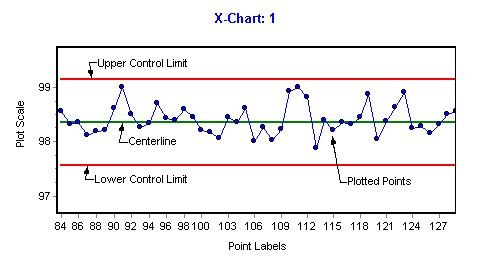
\includegraphics[height=0.3\textheight]{art/X-chartExample}
\caption[\barxChart]{\barxChart. \newline \url{https://mvpprograms.com/help/P-mvpstats/spc/WhatAreControlCharts}}
\label{fig:bar_x_chart}
\end{figure}






Figure~\ref{fig:bar_x_chart} makes it evident \barxChart requires several design decisions.
A standard design decision is setting the center line as the grand average of the process: 
\begin{align}
\label{eq:centerline}
	1/\tau \sum_{t=1}^\tau \bar{x}_t
\end{align}


If it is unclear to you, how may we compute the grand average of a process that is still evolving and has not finished, you are right! We thus introduce the ideas of \emph{Phase I} and \emph{Phase II}. \marginnote{Phase I/II}
Initially we assume the process it out of control, we identify and remove assignable causes of variation, until we are left with a ``well-behaved'' subset of data points. We call this Phase I, and we use it to initialize required quantities such as the centre line. 
Eq.(\ref{eq:centerline}) thus implies that in Phase I we were left with $\tau$ samples assumingly in statistical control.
After the chart has been calibrated, and major assignable sources of variability removed, we can finally start monitoring the process, known as Phase II.



Other design decisions to be made are:
\begin{enumerate}
\item UCL and LCL \footnote{Do not confuse with USL and LSL!}.
\item Sample size in each sample.
\item Rational groupings (within-period sampling scheme).
\item Frequency of samples (between-period sampling scheme). 
\item Other stopping rules.
\end{enumerate}
These deign decisions ultimately govern the error rate (false positive rate) and power (false negative rate) of the chart, which in turn, incur some financial costs. 
For now we will restrict attention to type I/II error rates, until Section~\ref{sec:economical_considerations} where we consider these choices as economical optimization problems.

For ease of exposition, control chart design is demonstrated for the \barxChart, but equally apply to other control charts.
We start by a type I error rate analysis. 
Denote $\alpha_t$ the false alarm probability at period $t$.
How do our design choices affect $\alpha_t$?
\begin{align}
	\alpha_t &:= 1-P_{H_0}(\bar{x}_t \in [UCL,LCL]) \\
	&= 2 P_{H_0}(\bar{x}_t<UCL) \\
	&= 2 P_{H_0}(Z<\frac{UCL-\mu}{\sigma_{\bar{x}}}) \\
	&= 2 P_{H_0}(Z < -k) \\
	&= 2 \Phi(-k)
\end{align}
The above follows from assuming that $UCL:=\mu + k \sigmabar, LCL:= \mu - k \sigmabar$, $\x_{it}\sim \gauss{\mu,\sigma^2}$, and denoting $\sigmabar:= \frac{\sigma}{n}$.
A typical design choice is $k=3$, known as \emph{3-sigma control limits}, implying a false alarm rate of $\alpha_t=0.0027$.\marginnote{3-Sigma Control Limits}
Since we assumed the process is fixed over time, then so is $\alpha_t$ and we can simply write $\alpha_t=\alpha$.

A power analysis for our design choices follows the same lines.
Denote $\beta_t$, and $\pi_t=1-\beta_t$ the type II error rate, and power, at period $t$.
We then have
\begin{align}
	\pi_t &:= 1-P_{H_1}(\bar{x}_t \in [UCL,LCL])
\end{align}
and the rest follow from the distribution of $\bar{x}$ when the process is out of control.
Assuming the out-of-control process is a shift of magnitude $k \sigma$, i.e.: $\x \sim \gauss{\mu_1,\sigma^2}; \mu_1=k \sigma$, we plot in Figure~\ref{fig:power_function}, the detection power of a 3-sigma chart, as a function of $k$. 
This is known as statistical literature as a \emph{power function}, and in the engineering literature as the \emph{true positive rate} operator characteristic (TPR-OR.)


\begin{figure}[h]
\centering
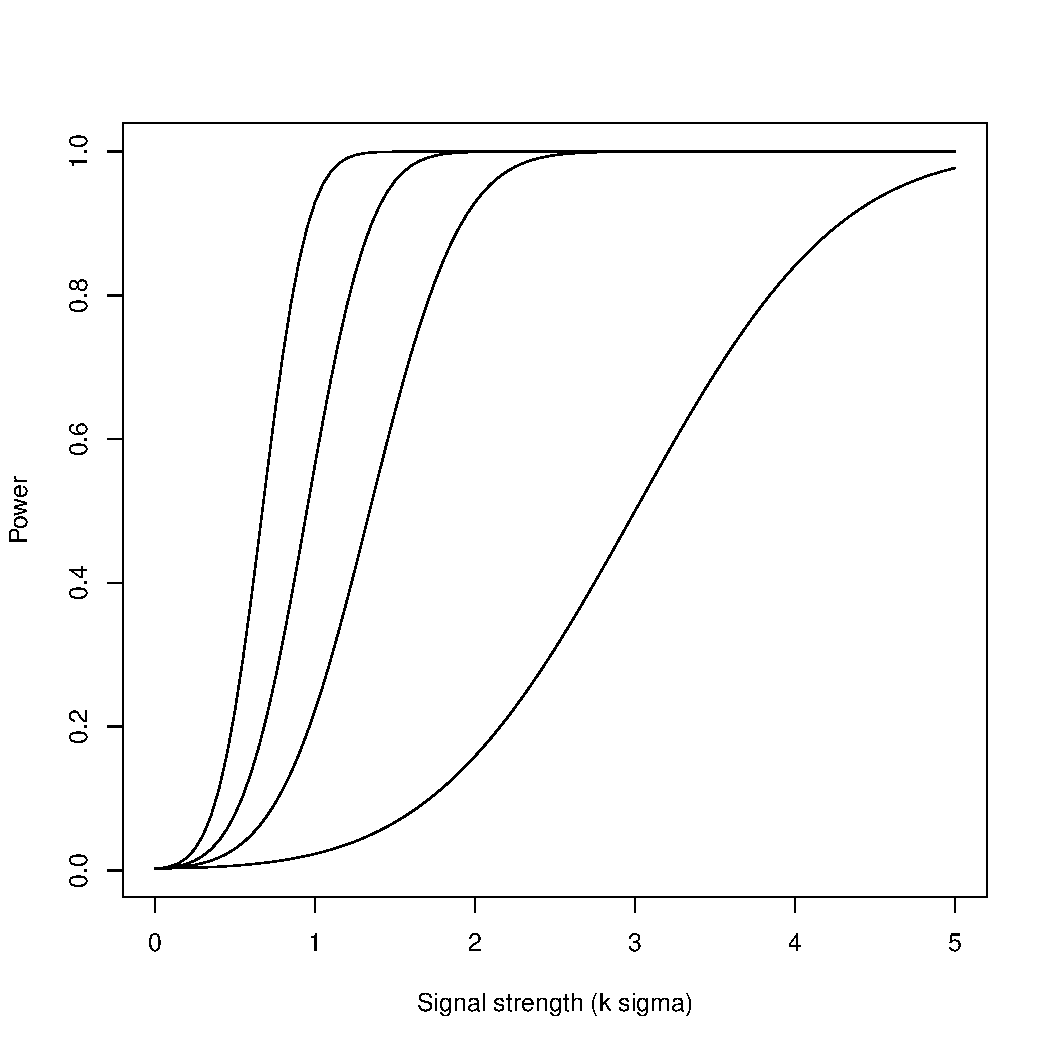
\includegraphics[height=0.3\textheight]{art/power_function.pdf}
\caption[Power Function]{Power function of the 3-sigma \barxChart with $n=5,10,20$ and $\mu_1=k \sigma$.}
\label{fig:power_function}
\end{figure}


\paragraph{ARL}
Another important related quantity is the \emph{average run length} (ARL), which is the expected number of periods between two crossings of control limits. \marginnote{ARL}
We denote by $ARL_0$ the average run length when the process is under statistical control, and $ARL_1$ otherwise\footnote{Note that it is implied that the process has a \emph{stable} distribution, even though it is out if control.}. 
If $\bar{x}_t$ are statistically independent, then clearly the number of periods until a crossing is geometrically distributed. Using the expectation of a geometric random variable we can conclude that 
\begin{align}
	ARL_0=1/\alpha \label{eq:arl_0} \\
	ARL_1=1/\pi \label{eq:arl_1}
\end{align}
Clearly we can convert to time units by multiplying the ARL by the duration of sampling interval.
This is known as the \emph{average time to signal} (ATS).\marginnote{ATS}


Now assume that we are unhappy with some control chart. 
It simply makes too many false alarms, or takes too long to detect loss of statistical control.
What can we do about it?
Well, this is exactly the same question as when increasing the power or lowering the type I error of a statistical hypothesis test. This is obviously no coincidence, since control charts are nothing but a statistical test!
Here are some action courses:
\begin{enumerate}
\item Increase $k$. This is the same as shrinking a rejection region: 
it will decrease the false alarm rate, at the cost of statistical sensitivity.
\item Increase $n$. Brilliant! Statistically, there is nothing to lose. It may, however, cost time and money.
\item Increase the sampling frequency. Brilliant again! Nothing to lose, except time and money...
\item Change the sampling scheme within period. We elaborate on this in Section~\ref{sec:rational_grouping}.
\item Add other stopping rules: 
this acts just like growing a rejection region. It will increase power, at the cost of type I error. We elaborate in Section~\ref{sec:stopping_rules}.
\item Pool together more time points or more variables. We elaborate on this in sections \ref{sec:running_windows} and  \ref{sec:multivariate}, respectively. 
\end{enumerate}






\subsection{Control Limits and the Alarm Rate}
As previously discussed, $k$ governs the tradeoff between type I and type II errors, or sensitivity versus specificity.
It is very common to set $k=3$. 
For a Normally distributed CTQ, this implies $2,700$ false alarms per million periods. 
This also implies an ARL of $1/\alpha=370$ periods.
We may however, discard this convention, and directly set UCL and LCL so they guarantee some desirable false alarm rate. 

If normality of $\bar{x}$ can be assumed, then one may estimate $\sigma$ from phase I, and set LCL and UCL by finding the $k$ that solves $2\Phi(-k)=\alpha$.
If normality cannot be assumed, there are many ways to go about. Here are some options:
\begin{enumerate}
\item Increase $n$: even if $\x_i$ is non normal, for large enough $n$, then $\bar{x}$ will be via the central limit theorem.
\item Use empirical quantiles: If phase I was returned enough data, then we may estimate $\x_{\alpha/2}$ and $\x_{1-\alpha/2}$ using the empirical quantiles of phase I. The false alarm rate will be $\alpha$ since $P(\x \not \in [\x_{\alpha/2},\x_{1-\alpha/2}])=\alpha$, if $[\x_{\alpha/2},\x_{1-\alpha/2}]$ is well estimated.
\item TODO:simulation
\end{enumerate}




\subsection{Rational Groupings}
\label{sec:rational_grouping}
Recall that at each period we compute the average of $n$ samples. 
How should we draw this samples? All at the same time from the same machine?
At different times from the same machine?
Many configurations are possible, and the correct approach depends on the type of out-of-control behaviour one seeks. 
\emph{Rational groupings} merely reminds us to sample ``rationally'' in each period. 
Quoting \cite{montgomery_introduction_2007}'s words of caution:
\begin{quotation}
\dots we can often make any process appear to be in statistical control just by stretching out the interval between observations in the sample.
\end{quotation}






\subsection{Other Stopping Rules}
\label{sec:stopping_rules}

The assumption that we may only create alarms if $\bar{x}$ exceeds some control limits is needle sly restrictive.
A first relaxation is by allowing multiple regions.
It is quite common to define \emph{warning limits} which only call for inspection, and \emph{action limits}. Each may have its own alarm rate.
We may even change the sapling scheme if limits are breached. Increasing the sampling rate once the warning limits have been breached is known as \emph{adaptive sampling}, or \emph{variable sampling}.\marginnote{Adaptive Sampling}



Another, more strict approach, is to define multiple sets of stopping rules
Here an example:
\begin{enumerate}
\item One or more points outside of the control limits.
\item Two of three consecutive points outside the 2-sigma warning limits but still inside the control limits.
\item Four of five consecutive points beyond the 1-sigma limits.
\item A run of 8 consecutive points on one side of the center line.
\end{enumerate}
The above set of rules is known as the Western Electric Rules, \aka\, the \emph{WECO} rules.\marginnote{WECO}
Augmenting the set of rules is the same as increasing a rejection region. It adds more sensitivity, at the cost of false alarms. If the rules are properly selected, the gain in sensitivity is worth the increase in false alarms.

As a quick exercise, we may compute $\alpha$  for $m$ independent rules, each with $\alpha^*$ type I error itself:
\begin{align}
	\alpha=1-(1-\alpha^*)^m.
\end{align}
Having 4 rules, like WECO, each at $\alpha^*0.0027$ implies that we actually have $\alpha=0.01$.

\begin{extra}[Stopping Rules]
There are many sets of stopping rules. 
These include WECO, Nelson, AIAG, Juran, Hughes, Duncan, Gitlow, Westgard, and more. 
See \url{http://www.quinn-curtis.com/spcnamedrulesets.htm} for a quick introduction.
\end{extra}



\section{Pooling Information Over Periods}
\label{sec:running_windows}

Assume an out-of-control process is simply a mild shift of the controlled-process.
This shift may be hard to detect in Shewart chart, especially if $n$ is not too large (as seen in Figure~\ref{fig:power_function}).  
If the shift persists, we may gain power, i.e., sensitivity, by pooling several periods together. 
We now present several ways to pool information from history. These are typically applied in Phase II, where out-of-control processes are expected to have only mild shifts, and not major ones as in Phase I. 



\subsection{Moving Average Chart- MA}
One way to pool information from different periods is by a \emph{moving average}.
\begin{definition}[Moving Average]
The moving average at period $t$ is defined as
\begin{align}
	M_t:= \frac{\bar{x}_t+\dots+\bar{x}_{t-w+1}}{w}
\end{align}
\end{definition}
Assuming $\bar{x}_t \sim \gauss{\mu_0, \sigma^2/n}$ then clearly 
\begin{align}
	M_t \sim \gauss{\mu_0, \frac{\sigma^2}{nw}}.
\end{align}
It is quite advantageous, and common, to take one observation at a time, so that $n=1$.

The control limits on $M_t$ are typically
\begin{align}
	UCL &:= \mu_0 + 3 \sigma_{M_t}= \mu_0 + 3 \, \frac{\sigma_x}{\sqrt{nw}} \\
	UCL &:= \mu_0 - 3 \sigma_{M_t}= \mu_0 - 3 \, \frac{\sigma_x}{\sqrt{nw}}.
\end{align}
The fallout rate of this criterion is trivially $\alpha=0.0027$. 
The ARL, however, is no longer so simple to compute. 
This is because the pooling of periods has violated the independence between periods, and Eqs.(\ref{eq:arl_0},\ref{eq:arl_1}) are no longer valid. 
Do not despair, however, as the ARL may still be computed. 
You can always use simulation to compute it, or try using the \rcode{spc} \R package.


%\begin{algorithm}[$ARL_0$ simulation for MA Control Chart]
%\caption{$ARL_0$ simulation for MA Control Chart}
%\begin{algorithmic}
%\For {$\bootstrap \in 1,\dots,\bootstraps$}
%	\State $\sample^\bootstrap \gets$ $n$ randomly selected observations, with replacement, from the original data.
%	\State $\sample^\bootstrap_\rank \gets$ $\rank$ randomly selected variables from $\sample^\bootstrap$.
%    \State $\estim{\hyp}^{\bootstrap} \gets$ a tree learned with  $\sample^\bootstrap_\rank$.
%\EndFor
%\State \Return the the average prediction for $x$ over $\estim{\hyp}^{\bootstrap}$ .
%\end{algorithmic}
%\end{algorithm}


We are free to choose the magnitude of $w$. If $w$ is too small, there is no real pooling from history. At the limit, where $w=1$, we are back to the classical Shewart chart. 
If $w$ is too large, then each new observation has very small importance, and it may take a long time to detect a shift.
Which is the right intermediate value, is left for you to decide.






\subsection{Exponentially Weighted Moving Average Chart- EWMA}
The moving average gives all observations the same importance. 
We want to change this, so that we may capture drifts quickly when they occur, while enjoy the power benefits that come with pooling information over periods. 
The \emph{Exponentially Weighted Moving Average} (EWMA), \aka the \emph{geometric moving average} (GMA), does just that. 
\begin{definition}[Exponentially Weighted Moving Average- EWMA]
\begin{align}
	z_t:= \lambda \bar{x}_t + (1-\lambda) z_{t-1}
\end{align}
\end{definition}
%By recursive substitution, we have 
%\begin{align}
%	z_t:= \lambda \sum_{j=0}^{t-1} (1-\lambda)^j \bar{x}_{t-j} + (1-\lambda)^t z_0
%\end{align}

By recursive substitution we have that 
\begin{align}
\label{eq:ewma_variance}
	\sigma^2_{z_t}=\frac{\sigma^2_x}{n}\left( \frac{\lambda}{2-\lambda} \right)(1-(1-\lambda)^{2t}),
\end{align}
and 
\begin{align}
	z_t \sim \gauss{\mu_0,	\sigma^2_{z_t} }.
\end{align}
Eq.(\ref{eq:ewma_variance}) may be used to construct control limits for EWMA:
It is however, more economic to observe that for large $\lambda$ and $t$: $(1-(1-\lambda)^{2t}) \approx 1$ so that we may use 
\begin{align}
\begin{split}
\label{eq:ewma_variance_approximate}
	UCL &:= \mu_0 + 3 \sigma_{z_t}= \mu_0 + 3 \, \sqrt{\frac{\sigma^2_x}{n}\left( \frac{\lambda}{2-\lambda} \right)},  \\
	UCL &:= \mu_0 - 3 \sigma_{z_t}= \mu_0 - 3 \, \sqrt{\frac{\sigma^2_x}{n}\left( \frac{\lambda}{2-\lambda} \right)}.
\end{split}
\end{align}
By now, you should immediately know what is the fallout rate of these limits.
By now, you should also know that because of the dependence between $z_t$'s, computing the ARL is not as simple as for Shewart charts. The \rcode{xewma.arl()} \R function, in package \rcode{spc}, permits doing so easily. 
Its output for various $\lambda$ and $k$ is illustrated in Figure~\ref{fig:arl_0_ewma}.

\begin{figure}[h]
\centering
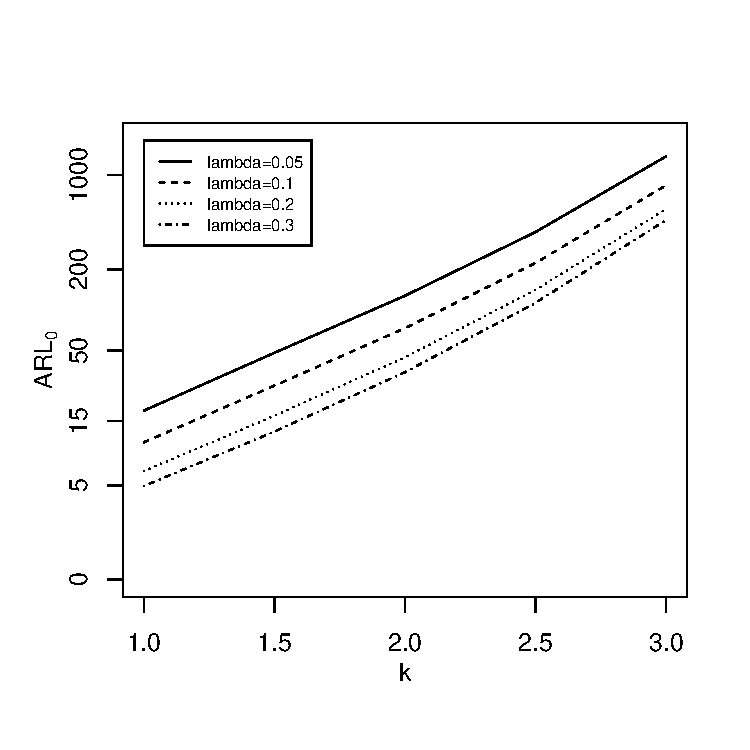
\includegraphics[height=0.3\textheight]{art/fig53}
\caption[$ARL_0$ for EWMA]{$ARL_0$ for EWMA. \newline Code from \url{http://users.phhp.ufl.edu/pqiu/research/book/spc/r-codes/fig53.r}}
\label{fig:arl_0_ewma}
\end{figure}

Note that if we do not opt for the approximation in Eq.(\ref{eq:ewma_variance_approximate}), and use the exact Eq.(\ref{eq:ewma_variance}) then the alarm limits change over time. 


In the MA chart, we used the choice of $w$ to balance between quick response (small $w$) and sensitivity (large $w$).
EWMA has no window-width parameter, since it looks on all of the history. On the other hand, we can control it by choosing $\lambda$. 
Large $\lambda$ gives more importance to the present. At the limit, $\lambda=1$, EWMA collapses to a standard Shewart chart.







\subsection{Filtered Derivative Chart}
[TODO]


\subsection{CUSUM Chart}
The \emph{cumulative sum} chart is similar to the EWMA in that it pools information from the history. 
It does differ, in that it gives all the history an equal weight. 
The CUSUM simply sums deviations from the centre line.
If the process is in control, deviation will cancel each other, and their sum will vary around $0$. 
If the process is ot of control, some drift will appear. 
The statistic to be plotted is 
\begin{align}
	C_t:= \sum_{j=0}^{t}(\bar{x}_j-\mu_0)=C_{t-1}+ (\bar{x}_t-\mu_0)
\end{align} 
Observing that when under control then $C_t \sim \gauss{\mu_0, \frac{t}{n} \sigma_x^2}$, we could set 
\begin{align}
\begin{split}
	UCL &:= \mu_0 + 3 \sigma_{C_t}= \mu_0 + 3 \, \sqrt{\frac{t}{n} \sigma_x^2},  \\
	UCL &:= \mu_0 - 3 \sigma_{C_t}= \mu_0 - 3 \, \sqrt{\frac{t}{n} \sigma_x^2}.
\end{split}
\end{align}
This approach, is rarely seen in practice, because it is suboptimal.
Indeed, 




%\begin{extra}[Wald's Sequential Likelihood Ration Test- SPRT]
%[TODO]
%\end{extra}




\subsection{Combined Shewart and Running Window Charts}






\begin{extra}[Local Methods]
% scan statistic
% sliding window
% search light
% Anomaly detection active learning
\end{extra}








\section{Multivariate Control Charts}
\label{sec:multivariate}
% Wishart
% Srivastava Du
% PCA
% Higher criticism




\section{Economical Design of Control Charts}
\label{sec:economical_considerations}






\section{Non-Statistical Target Functions}






\section{Other Control Statistics}
\subsection{$R$ Chart}
\subsection{$s$ Chart}
\subsection{$s^2$ Chart}
\subsection{Shewhart Individuals Control Chart}
\subsection{Three-way Chart}
\subsection{$p$ Chart}
\subsection{$np$ Chart}
\subsection{$c$ Chart}
\subsection{$u$ Chart}
\subsection{Time Series Model}
\subsection{Regression Control Chart}
\subsection{Running Window Versions}




\section{Notes}
% White noise process
% One sided control chart






% % % % DOE
\chapter{Design of Experiments}
\chaptermark{DOE}

This chapter is devoted to the matter of designing experiments, and follows the lines of \cite{cox_theory_2000}.
A control chart may be seen as an on-line experiment alerting us when the milk goes sour, but it will not tell us why. 
When designing a product (remember DFSS \ref{sec:dfss}), or once a control chart has signalled an alert, we will want to know what has influences our production, and how to remove variability.
In our SPC terminology, we will want to know what are the \emph{causal} \emph{effects} of our \emph{controllable inputs} (or \emph{factors}), on our \emph{CTQ} (or \emph{response}). 
The theory of discovering these effects is the theory of \emph{design of experiments} (DOE).
Its goal is to \emph{screen} factors with no effect, to estimate effect sizes, and find optimal factor-level combinations, and remove assignable variability; all these as efficiently as possibly.



Roughly speaking, the challenges in designing good experiment are:
\begin{enumerate}
\item Efficiency: extract the most information per sampled unit.
\item Signal to noise: remove variability that might mask factor effects.
\item Bias: avoid uncontrolled effects from being ``absorbed'' into controlled ones.
\end{enumerate}





Before we dig in, several matters should be emphasized:
\begin{description}
\item [Randomization] Randomization is fundamental to our purpose. This is because the idea of an \emph{effect} implies causality. Any inference we make, is causal, which is the inference we need for controlling a process.
It is the mechanism of randomization, that allows us to conclude that correlations are causal, and not merely statistical.
For a treatment of causal inference in \emph{observational data}, i.e., without randomization, see \cite{rosenbaum_observational_2002}.

\item [Pre-experiment] In this text we take it for granted that the purpose of the experiment is well known, and the candidate factors defined. We are fully aware, as should be the reader, that in application this is a non-trivial luxury. Indeed, a lot of planning, and domain-knowledge go into the selection of factors, their candidate levels, etc.

\item [Power Analysis] Part of the pre-experiment may include a power analysis. The pre-experiment power analysis will typically be very approximate, and rely on many assumptions. It is still important, as it gives an idea of the feasibility of an experiment, and avoids wasting resources.

\item [No Textbook Solution] We will present many design ideas and principles, yet it should be emphasized that real life problems rarely obey text-books. You should thus feel free, and even obliged, to think about your particular problem and adapt the experiment as you best see fit. 

\item[Data Analysis]
In this text, we only discuss the \textbf{design} of the experiment, and not the \textbf{analysis} of the data.
This is a non-standard choice as DOE is typically presented alongside the \emph{analysis of variance} (ANOVA) framework.\marginnote{ANOVA}
We decouple the two since: 
\cite{cox_theory_2000} do so, 
these are two different thing, and finally because the ANOVA framework may be easily replaced by the framework of \emph{linear models}, \emph{mixed models}, \emph{variance components}, and possibly others. 
There is a vast literature focusing on the analysis method. \marginnote{Linear Models, \\ Mixed Models, Variance Components}
If asked, this author may recommend \cite{hocking_analysis_1985}, which presents both the ANOVA terminology, and the linear models terminology.
That book, however, may be hard to come by, so feel free to ask me for other references if required.

\end{description}








\section{Terminology}
The following list is compiled from \cite{mason_statistical_2003}. Many, if not most of the following terms, originate in R.A. Fisher's seminal book ``The Design of Experiments'' \citep{fisher_design_1960}. As usual, when old ideas get new names, we try to emphasize this in the text.



\begin{description}

\item [Experimental Unit]  Entity on which a measurement or an observation is made;
sometimes refers to the actual measurement or observation.
\item [Homogenous Experimental Unit] Units that are as uniform as possible on all characteristics that could affect the response.

\item [Factors]  A controllable experimental variable that is thought to influence the response. In the language of SPC: \emph{a controllable input}.

\item [Level] Specific value of a factor.

\item[Treatment] The particular factor-level combination applied to an experimental unit. \Aka \emph{manipulation}, or \emph{cell}.

\item [Factor Encodings] The numerical encoding of factor levels.
Of minor importance for designing. Of major importance for analysis.
Two level factor encodings include:
\begin{enumerate}
\item Effect coding: where levels are encoded with $\set{-1,1}$.
\item Dummy coding: where levels are encoded with $\set{0,1}$.
\end{enumerate}

\item [Experimental Region] All possible factor–level combinations for which experimentation is possible. \Aka \emph{factor space}, and \emph{design region}.

\item [Design Matrix] A matrix description of an experiment that is useful for constructing and analyzing experiments.

\item [Response] The CTQ in the SPC literature. 

\item [Main Effect] Change in the expected response between two factor–levels.  
We emphasize that effects, unlike simple population parameters, imply a causal relationship.
Part of the \emph{assignable causes} in the SPC literature.

\item [Interaction] Existence of joint factor effects in which the effect of each factor depends on the levels of the other factors.
Part of the \emph{assignable causes} in the SPC literature.

\item [Noise] \Aka \emph{error}. The part of the response that cannot be attributed to any factors.
This is the \emph{common} variability in the SPC literature.

\item [Replication] Repetition of an entire experiment or a portion of an experiment under two or more sets of conditions.

\item [Covariate]  An uncontrollable variable that influences the response but is unaffected by any other experimental factors.
\Aka an \emph{exogenous} variable in the econometric literature.

\item [Design]  Complete specification of experimental test runs, including blocking, randomization, repeat tests, replication, and the assignment of factor–level combinations to experimental units.

\item [Blocking]  Blocking, or \emph{grouping}, is an experimental design technique that removes excess variation by grouping experimental units or test runs so that those units or test runs within a block are more homogeneous than those in different blocks. Blocking attributes are also known as \emph{non specific factors}.\marginnote{Non Specific Factors}

\item [Confounding] When the design is such that several effects cannot be told apart. \Aka \emph{aliasing}.

\item [Repeat Tests] Two or more observations that have the same levels for all the factors, i.e., receive the same treatment.

\item [Balance] Some symmetry in the combinatorial design of the experiment. In its simplest interpretation, a design where an equal number of units is assigned to each treatment.

\item [Orthogonality]  Special simplifications of analysis and achievement of efficiency consequent on such \emph{balance}.
\end{description}








\section{Dealing with Variability}
\label{sec:variance_components}

The idea that random samples come with variability, or noise, should not be new to the reader.
In this section, we will try to decompose variability into it sources, and learn several techniques to reduce them. 
Starting with a motivating example.



\begin{example}[Web Design]
\label{eg:variance_components}
Consider the problem of optimizing a web site, or user interface, where individuals performance is measured by conversion rate (the probability of a new user to signup, purchase, etc).
Users' conversion is influenced by several factors:
The site's attributes,
the users' attributes, 
a user's affinity to a particular attributes,  
a user's mood, 
and endlessly many other things
How can we accurately optimize our site, in the presence of these variability sources?
The site's attributes are the \emph{factors} we want to study.
The users' attributes are \emph{covariates}. 
A user's affinity to the site's attributes is an \emph{interaction}. 
The users' mood is unobservable, thus a \emph{non-specific factor} we will try to either \emph{block} or \emph{balance}.
Any other variability, will be captured by the \emph{noise} term of the model. 
\end{example}


In this chapter we will learn many principled methods for the efficient design of experiments which allow us to remove effect-masking variability, avoid bias, and reduce costs.
You may, and should, think of this web design problem as we advance, since all the methods presented may be applied to it.



\subsection{Gage R\&R Studies}
R\&R stands for \emph{repeatability} and \emph{reproducibility}.
In the context of quality control\footnote{Beware that these words are used with different meanings by different communities.} repeatability is the variability under repeated measurement, and reproducibility is the variability when the same measurement is performed elsewhere (different lab, technician, etc.).
Gage R\&R experiments consist of performing several \emph{repeat tests}, and different replications, in order to assess R\&R, which can be thought of the assessment of the precision of the experiment. 



\subsection{Completely Randomized Designs}
In the simplest of designs, all experimental units are randomly assigned to treatments. 
This is typically easy to implement.
In Example~\ref{eg:variance_components} this would imply randomly assigning users to interfaces.
If you suspect, as you should, that we may reduce variability by grouping types of users together, keep reading.



\subsection{Randomized Block Designs}
The idea of \emph{blocking} is to replace the complete randomization scheme by a restricted randomization scheme so that variability can be reduced without introducing bias. 
The restricted randomization is created by \emph{grouping}, or \emph{blocking} groups of experimental units, and randomizing allocation within the group. 
In our running example, we could reduce the variability of the web site's attributes by showing various sites to the same person- each person would be his own block. This is an example of \emph{crossover} design, discussed in Section~\ref{sec:crossover}.
Alternatively, we could block individuals along, say, age group. Age would act as a a non-specific factor, and we would then randomly assign user's to sites, only within age groups.
If each age group has as many users as there are different site designs, this is a \emph{randomized complete block design}.\marginnote{Complete Block Design}
If there are less users then site designs, this is a \emph{incomplete block design}.
There are several approaches to incomplete block designs, but we refer the reader to \cite[Sec.4.2]{cox_theory_2000} for details.




\subsubsection{Latin Square Design}
When homogenous groups are defined by two non-specific factors, we would like to create blocks that are balanced, so that the non-specific factors do not bias effect estiamtes.
In our running example, non-specific factors may be age and gender. 
We could construct all age and gender combinations, and randomly assign users from each age-gender to each site design.
This would is an example of a \emph{split plot} design, discussed in Section~\ref{sec:split_plot}.
If, however, we do not deal with age-gender, but rather with age-country, we may not have enough users in each cell to assign to all site designs. 
Since we do not want to estimate the effect of age, nor country, but merely balance the design so that age and country effects do not alias the site's effect, we do not actually need all age-country combinations. 



If we have $k$ designs, we may group ages and countries into $k$ categories each, and each design is seen only once in each age group and once in each country group. 
This allocation of treatment to blocks is known as a \emph{Latin Square}. 
Table~\ref{tab:latin_square} demonstrates a Latin Square for $7$ web site designs, and compares it to a non-balanced allocation. 
\begin{table}[ht]
    \begin{minipage}{.5\linewidth}
        \centering
		\begin{tabular}{rlllllll}
		  \hline
		 & 1 & 2 & 3 & 4 & 5 & 6 & 7 \\ 
		  \hline
		1 & 1 & 2 & 3 & 4 & 5 & 6 & 7 \\ 
		2 & 1 & 2 & 3 & 4 & 5 & 6 & 7 \\ 
		3 & 1 & 2 & 3 & 4 & 5 & 6 & 7 \\ 
		4 & 1 & 2 & 3 & 4 & 5 & 6 & 7 \\ 
		5 & 1 & 2 & 3 & 4 & 5 & 6 & 7 \\ 
		6 & 1 & 2 & 3 & 4 & 5 & 6 & 7 \\ 
		7 & 1 & 2 & 3 & 4 & 5 & 6 & 7 \\ 
		   \hline
		\end{tabular}
    \end{minipage}%
    \begin{minipage}{.5\linewidth}
      \centering
		\begin{tabular}{rlllllll}
		  \hline
		 & 1 & 2 & 3 & 4 & 5 & 6 & 7 \\ 
		  \hline
		1 & 1 & 2 & 3 & 4 & 5 & 6 & 7 \\ 
		  2 & 2 & 3 & 4 & 5 & 6 & 7 & 1 \\ 
		  3 & 3 & 4 & 5 & 6 & 7 & 1 & 2 \\ 
		  4 & 4 & 5 & 6 & 7 & 1 & 2 & 3 \\ 
		  5 & 5 & 6 & 7 & 1 & 2 & 3 & 4 \\ 
		  6 & 6 & 7 & 1 & 2 & 3 & 4 & 5 \\ 
		  7 & 7 & 1 & 2 & 3 & 4 & 5 & 6 \\ 
		   \hline
		\end{tabular}
		\end{minipage} 
\caption{A $7$-treatment, two-factor design. 
Left pane is not balanced.
Right pane is balanced with a Latin Square, generated with the \rcode{MOLS()} function of the \rcode{crossdes} \R package.}
\label{tab:latin_square}		
\end{table}


The following example makes the same point, with the original agricultural motivation for this design.
\begin{example}[Agricultural Yield Study]
\label{eg:latin_square}
Consider an farmer growing corn.
He wishes to study the effect of $7$ candidate fertilizers (single factor with $7$ levels).
He is aware that the location of the plot may affect yield, due to slightly different sunlight, irrigation, altitude, etc.
He thus assumes he has to deal with two extra variance sources: row and column of the plot. 
He could treat the row and column as two factors, with $7$ levels each, be he does not care to estimate the row/column effect, but merely to avoid bias.
He will thus try to look for an allocation of fertilizer to rows and columns so that any row/column effect will be averaged out.
The Latin Square design of Table~\ref{tab:latin_square} does just that.
\end{example}


\begin{extra}\noindent
\begin{enumerate}
\item If the Latin Square reminds you of Soduko, it should. Soduko is just that!
\item The Latin Square is a very economical design, and is not used as often as it should be.
\item If we had reason to believe that different age groups in different countries respond differently to each site (an interaction), then the Latin Square may actually introduce aliasing. 
\end{enumerate}
\end{extra}



\subsubsection{Extensions of the Latin Square}
\begin{enumerate}
\item \textbf{Latin Hypercube}: When balancing more than two non-specific factors, we will call upon \emph{latin hypercube designs}, \aka \emph{orthogonal latin squares}. \marginnote{Orthogonal Latin Squares}
\item \textbf{Greco-Latin Square}: A latin-hypercube with three variability sources. 
\end{enumerate}






\subsubsection{Crossover Design}
\label{sec:crossover}
Lets return to the web site layout example (\ref{eg:variance_components}).
Let us also assume that our site has $3$ web pages. A landing page, an information page, and a form to fill. 
It is possible that the response to a particular page is affected by the previous page presented. 
This is known as a \emph{carryover effecf}, or \emph{residual effect}, which may bias the main layout effects of interest. \marginnote{Carryover Effect}

The more general phenomenon is dependence in the noise between trials. 
Consider the same subject undergoing different treatments, or adjacent fields. 
\emph{Crossover} designs are such that all possible treatment adjacencies are considered, so that the carry over effect averages out. 

In a \emph{fully randomized crossover design}, each unit is randomly allocated to a sequence of treatments.
If treatments are combinations of several factors, it is not uncommon to use Latin Squares to generate the sequences. Table~\ref{tab:crossover} demonstrates the $3!=6$ sequences for our $3$ page website problem.
\begin{table}[ht]
\centering
\begin{tabular}{rlll}
  \hline
 & 1 & 2 & 3 \\ 
  \hline
1 & 1 & 2 & 3 \\ 
  2 & 2 & 3 & 1 \\ 
  3 & 3 & 1 & 2 \\ 
  4 & 1 & 3 & 2 \\ 
  5 & 2 & 1 & 3 \\ 
  6 & 3 & 2 & 1 \\ 
   \hline
\end{tabular}
\caption[Crossover Design]{Crossover design: a balanced sequence of administration of $3$ treatments, generated with the \rcode{des.MOLS()} function of the \rcode{crossdes} \R package. }
\label{tab:crossover}
\end{table}






\section{Factorial Designs}
Until now we discussed some arbitrary set of treatments.
It is quite common, is not certain, that the many treatments are merely combination of a small number of \emph{factors} with a small number of \emph{levels} each.
This means that we may decompose treatment effect into the (partial) sums of the effects of underlying factors, which would make both the design more economical, and the analysis easier to interpret.

We will now present several designs for factorial experiments.
Recall that factors define treatments. The noise reducing and bias avoiding methods of Section~\ref{sec:variance_components} may thus be compounded with the treatment generating methods of this section.

It should be emphasized that a factorial design is better than $k$ experiments with one factor at a time. This is because:
\begin{enumerate}
\item Factorial experiments are make better (statistical) use of each sample unit for estimating main effects.
\item Factorial experiments allow the estimation of interactions between factors. 
\end{enumerate}
A classical illustration of the second point, is given in Figure~\ref{fig:one_factor_at_a_time}.
The figure depicts a one-factor-at-a-time optimization sequence (from A to H). Since the factors are not varied simultaneously, the experiments is unable to identify that the response is not a linear surface. 
Put differently, he is unable to estimate an interaction.

\begin{figure}[ht]
\centering
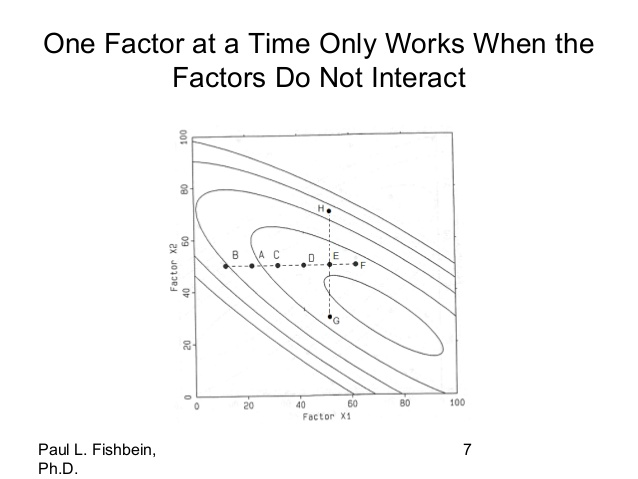
\includegraphics[height=0.3\textheight]{art/optimization-without-statistical-doe-2015-03-23-7-638}
\caption{Optimizing factors, one at a time.\newline \url{http://www.slideshare.net/PaulFishbein/optimization-without-statistical-doe-2015-03-23-46817073}}
\label{fig:one_factor_at_a_time}
\end{figure}




\subsection{Full Factorial Designs}
A \emph{full factorial}, or \emph{complete factorial} design, is one where all factor-level combinations are replicated the same number of times.
The most common of the full-factorial designs is the $2^k$-design where all combinations of $k$ factors with two levels each are tested in each replication.



\subsubsection{$2^k$ design}
Consider two factors denoted $A$ and $B$.
Adopt the effect coding so that we encode their levels by $\set{-1,1}$.
The design matrix of a single run is depicted in Figure~\ref{fig:full_factorial} (top right) along with a visualization of the design (top left).
Allowing $n$ observations per condition, the experiment will include $4n$ observations, which will be randomized between conditions.

\begin{figure}[ht]
\centering
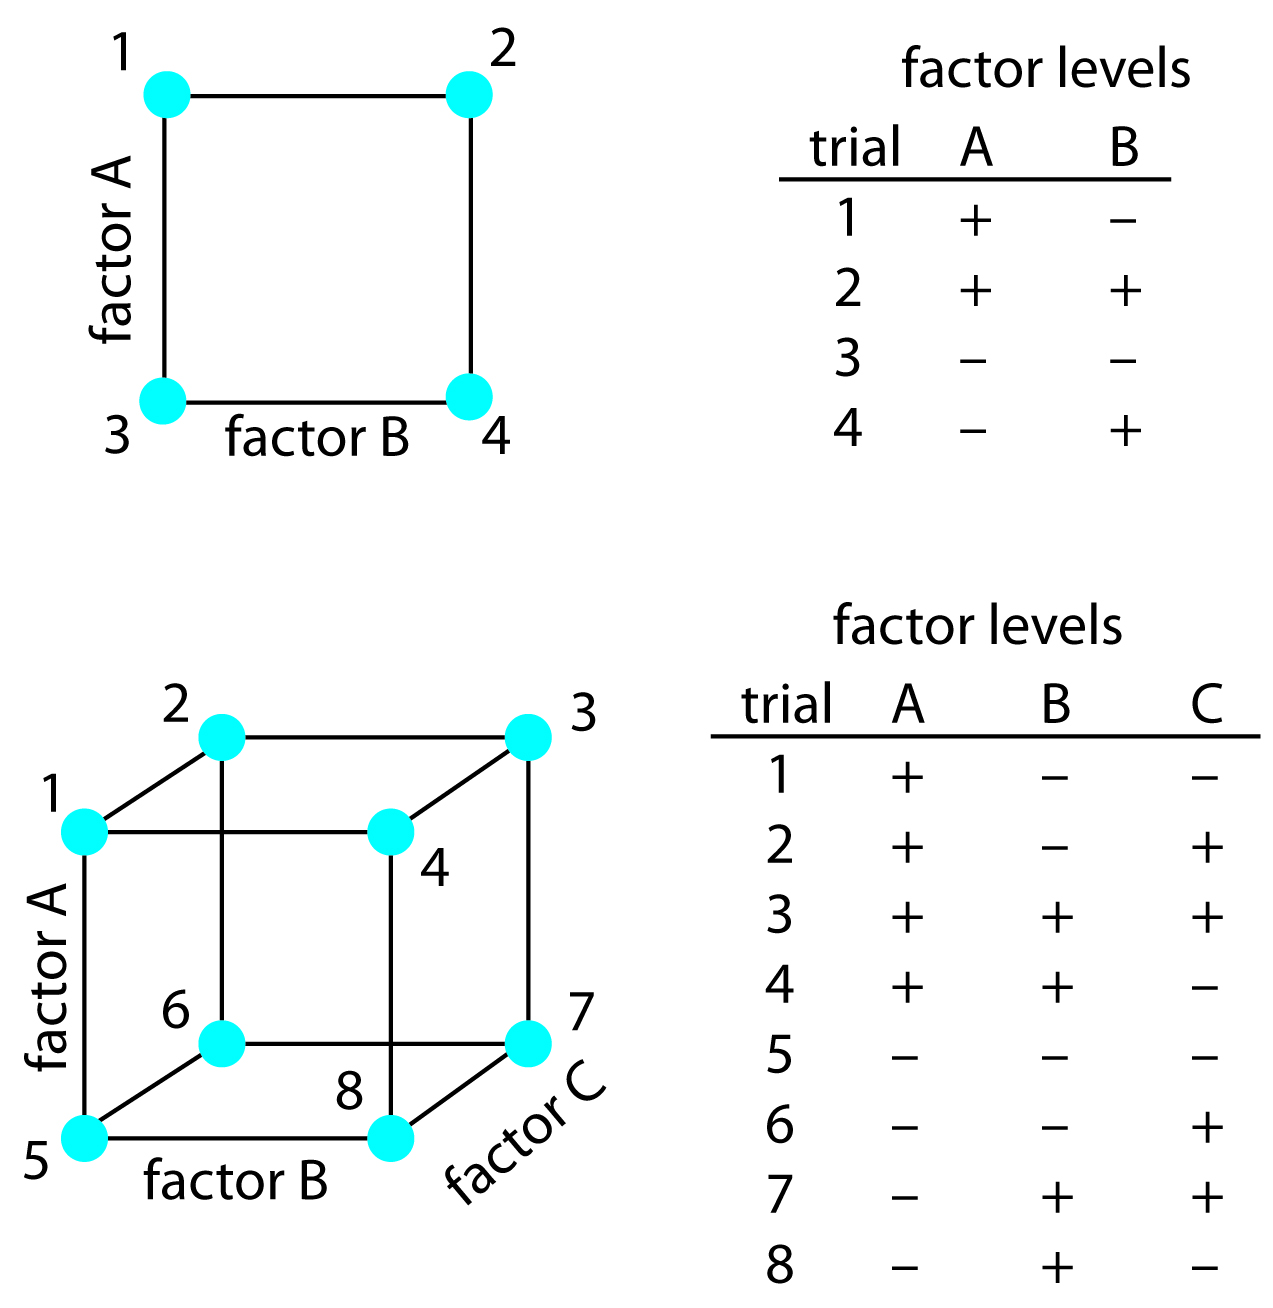
\includegraphics[width=0.7\linewidth, height=0.3\textheight]{art/full_factorial}
\caption[Full Factorial Design]{Full factorial designs: $2^2$ and $2^3$. \newline \url{http://chemwiki.ucdavis.edu/Analytical_Chemistry/Analytical_Chemistry_2.0/14_Developing_a_Standard_Method}}
\label{fig:full_factorial}
\end{figure}
With this $2^2$ design, we may recover several effects:
\begin{description}
\item [Main effect of A] The effect of varying $A$ from $(-)$ to $(+)$, denoted $\tau^A$.
\item [Main effect of B] The effect of varying $B$ from $(-)$ to $(+)$, denoted $\tau^B$.
\item [Main effects and interaction] The effect of varying both $A$ and $B$ from $AB=(--)$ to $AB=(++)$, , denoted $\tau^{AB}$.
\end{description}

We typically denote
\begin{table}[H]
\centering
\begin{tabular}{|c|c|c|c|}
\hline Treatment & A & B & Mean \\ 
\hline 1 & + & - & $\mu_a$ \\ 
\hline 2 & + & + & $\mu_{ab}$ \\ 
\hline 3 & - & - & $\mu_{(1)}$ \\ 
\hline 4 & - & + & $\mu_b$ \\ 
\hline 
\end{tabular} 
\end{table}
How are these effects related to the mean responses to each treatment?
\begin{align}
	\tau^A &:= \frac{1}{4}\left( (\mu_{ab}+\mu_a)- (\mu_{(1)}+\mu_b)\right), \\
	\tau^B &:= \frac{1}{4}\left( (\mu_{ab}+\mu_b) - (\mu_{(1)}+\mu_a)  \right), \\
	\tau^{AB} &:= \frac{1}{4}\left( \mu_{ab} +  \mu_{(1)} -  \mu_a - \mu_b \right).	
\end{align}



\marginnote{Interaction}

Slightly intruding into the realm of data analysis, a visualization of interactions is known as the \emph{interaction plot}, depicted in Figure~\ref{fig:interaction_plot}. 
The upper left panel demonstrates a lack of interaction (think why), while the upper right panel depicts an interaction.
\begin{figure}[ht]
\centering
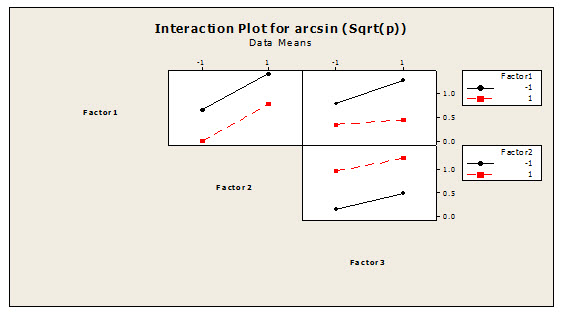
\includegraphics[width=0.3\textheight]{art/attribute_doe_interaction_plot}
\caption[Interactions plot]{Interactions plot. \newline \url{http://blog.minitab.com/blog/statistics-in-the-field/optimizing-attribute-responses-using-design-of-experiments-doe-part-2}}
\label{fig:interaction_plot}
\end{figure}


\begin{remark}[Screening Experiments]
The $2^k$ designs are probably the most popular full factorial designs. 
This may be attributed to the fact that many factors studied really have two levels, but more plausibly, since these are merely \emph{screening} experiments. 
Once non related factors have been screened, the experimenter may proceed from the $2^k$ design to more elaborate ones. 
\end{remark}



\begin{remark}[Intermediate Factor Levels]
In a $2^k$ design, a factor may actually be a continuous controllable input which was restricted to two values for convenience. 
After estimating the effect of the factor, we may want to know what the effect would have been, had we set it on some intermediate level.
It is customary to assume that a main effect acts linearly in-between experimental conditions, yet you should remember that there is nothing in the data to support this.
For a more rigorous approach, see the Response Surface Methodology Section (\ref{sec:response_surface}).
\end{remark}


\begin{remark}[Crossed Treatments]
Both crossover designs and full factorial designs are \emph{crossed} in that all factor combinations are sampled. 
The difference is that in a full-factorial, a factor combination is applied simultaneously to an experiment unit, and in a crossover design, the application is sequential \citep{everitt_cambridge_2010}.
\end{remark}



\subsubsection{$3^k$ Designs}
I think that the name $3^k$ design is rather self explanatory.
Then again, more than $2$ levels are rarely treated as factorial experiments. 
This is because $3$ level factors typically appear when aiming at optimizing the factor combination, for which the \emph{response surface} methodology of Section~\ref{sec:response_surface} is more economical.




\subsection{Fractional Factorial}
The full factorial designs are the simplest designs to setup and interpret. 
A major drawback, are the resources required when $k$ is large. 
This is where the \emph{fractional factorial}, or \emph{partial factorial} designs kick in.
The fundamental idea is to design a full factorial, but skip a couple experimental conditions. If conditions to skip are wisely selected, only information on higher order interactions will be compromised.


\begin{example}[From $2^2$ to $2^{(2-1)}$]
\label{eg:fractional_factorial}
As a first example, we will try to save some time and money by eliminating particular conditions of the $2^2$ design in Figure~\ref{fig:full_factorial}.
As the name may suggest, a $2^{2-1}$ design, has $2$ experimental conditions in each run. 
There are thus $\binom{4}{2}=6$ possible eliminations.
\begin{table}[ht]
\begin{tabular}{|p{2.5cm}|p{10cm}|}
\hline Elimination &  Problem \\ 
\hline
\hline 1,2 &  No information on $a$. \\ 
\hline 1,3 &  No information on $b$.\\ 
\hline 1,4 &  $a$ aliased with $b$ aliased with $ab$. \\ 
\hline 2,3 &  $a$ aliased with $b$ aliased with $ab$. \\ 
\hline 2,4 &  No information on $b$. \\ 
\hline 3,4 &  No information on $a$.\\ 
\hline 
\end{tabular} 
\label{tab:partial_factorial}
\caption[Aliasing]{Aliasing in a $2^{2-1}$ design: All possible eliminations from the $2^2$ design that lead to a $2^{2-1}$ design.}
\end{table}
\end{example}

The lesson from Example~\ref{eg:fractional_factorial} is that in a fractional factorial our savings in time and money, come at the cost of the information that can be drawn from the experiment.
The idea behind partial factorial experiments, is that by an informed choice of the conditions skipped, we can choose what information to give up. The information lost, is known as the \emph{alias structure}.\marginnote{Alias Structure}

In practice, we will rarely do the actual elimination of conditions, but rather revert to pre-selected designs. 
Table~\ref{tab:partial_factorial_ii}, generated with the \rcode{FrF2()} in the \rcode{FrF2} \R package, is an optimal $2^{3-1}$ design.
Using the \rcode{design.info()} function of that same package, we know that the aliasing structure of this design is
$a=bd=ce, b=ad, c=ae, d=ab, e=ac$.
We will not go into the details of how the aliasing structure is computed, but rather refer the reader to \cite{cox_theory_2000}.
\begin{table}[ht]
\centering
\begin{tabular}{rrrrrr}
  \hline
 & A & B & C & D & E \\ 
  \hline
1 & -1 & 1 & -1 & -1 & 1 \\ 
  2 & 1 & -1 & 1 & -1 & 1 \\ 
  3 & -1 & -1 & -1 & 1 & 1 \\ 
  4 & -1 & 1 & 1 & -1 & -1 \\ 
  5 & -1 & -1 & 1 & 1 & -1 \\ 
  6 & 1 & 1 & 1 & 1 & 1 \\ 
  7 & 1 & -1 & -1 & -1 & -1 \\ 
  8 & 1 & 1 & -1 & 1 & -1 \\ 
   \hline
\end{tabular}
\label{tab:partial_factorial_ii}
\caption[Fractional Factorial Design]{$2^{5-2}$ design.}
\end{table}


\begin{definition}[Resolution of a Design]
As we have already seen, there are $\binom{2^k}{2^{k-p}}$ possible eliminations that convert a $2^k$ design to a $2^{k-p}$ design.
We call the \emph{resolution of the design}, the lowest order effect that is aliased. 
In Table~\ref{tab:partial_factorial_ii}, the resolution is 1, making it a rather unattractive design. 
Resolutions below 3 typically considered not informative, and above 5, considered wasteful.
\end{definition}


\begin{extra}[Coding Theory]
There is a close relationship between design of experiments and coding theory in computer science. 
A possible reference on the matter is \cite{hill_first_1986}, or \cite{hedayat_orthogonal_1999}.
\end{extra}



\subsection{Split Plot Design}
\label{sec:split_plot}
A \emph{split plot}, or \emph{split unit} design, is essentially a factorial design with blocking. 
It takes its name from farming plots: where these are used for blocking and split among the various treatments. 
The canonical example is due to \cite[Sec.12.4]{montgomery_design_2012}, and consists of studying two production factors with blocking by day. 
For more on split plots see \cite[Sec.6.4]{cox_theory_2000}.



\section{Continuous Factors}
When dealing with continuous factors, or \emph{quantitative factors}, we have many more analysis strategies than when dealing with qualitative factors.
No matter the analysis strategy, it is still important of choosing the right factor level combinations to study.

Clearly, we cannot identify nonlinearities when sampling a factor only a two levels.
We may thus opt for a full $3^k$ factorial design to fit a non-linear surface to the data.
The factor encoding would typically be $\{-1,0,1\}$,
A full $3^k$ factorial design may however be needlessly expensive. 
A more common approach in industrial application is the \emph{central composite design}, where a $2^k$ design is augmented with well chosen sampling points. \marginnote{Central Composite Design}
For more details see \cite[Sec.6.6]{cox_theory_2000}


\subsection{Response Surface Methdology}
\label{sec:response_surface}
As the name suggests, \emph{response surface methdology} deals with the estimation of the response surface to the levels of continuous factors.
Response surfaces are typically assume to be (approximately) quadratic, and experimentation typically conducted in stages. First screening factors, then fitting a surface, and finding optimal factor levels.



\subsection{Taguchi Methods}
Taguchi methods is a collective name for the philosophy, design, and analysis methods in industrial applications promoted by Genichi Taguchi in 1970's Japan.
Focusing on the design principles, we may note the following particularities of Taguchi's method:
\begin{enumerate}
\item Achieving low variability is more challenging then achieving a target value. 
\item Factors which can be controlled in a lab, but not in production, are deliberately varied. Typically in split plot  designs (\ref{sec:split_plot}).
\item Systematic use of latin hypercubes to study main effects and two-way interactions. Particularly \emph{Plackett–Burman designs}.\marginnote{Plackett Burman Design}
\item Log variability is often used as the response.
\end{enumerate}





\subsection{Optimal Designs}
% 1D least squares example
% pD least squares example
% logistic regression example


Our discussion until now has been informal with respect to the desirable qualities of a design. 
We used the idea of ``balance'' and ``orthogonality'' to avoid bias and unwelcome variability.
In this section, we try to formalize the notion of a ``good design''.
We start with some motivating examples.

\begin{example}[Design for non linear regression]
\label{eg:design_linear}
Figure~\ref{fig:design_linear} demonstrates the effect of the different location of the sampling points ($x$) on the quality of the estimated regression line, in a \textbf{linear} model.
As the figure depicts, it is preferable to spread the sampling points as far as possible, as intuition may suggest.
\begin{figure}[ht]
\centering
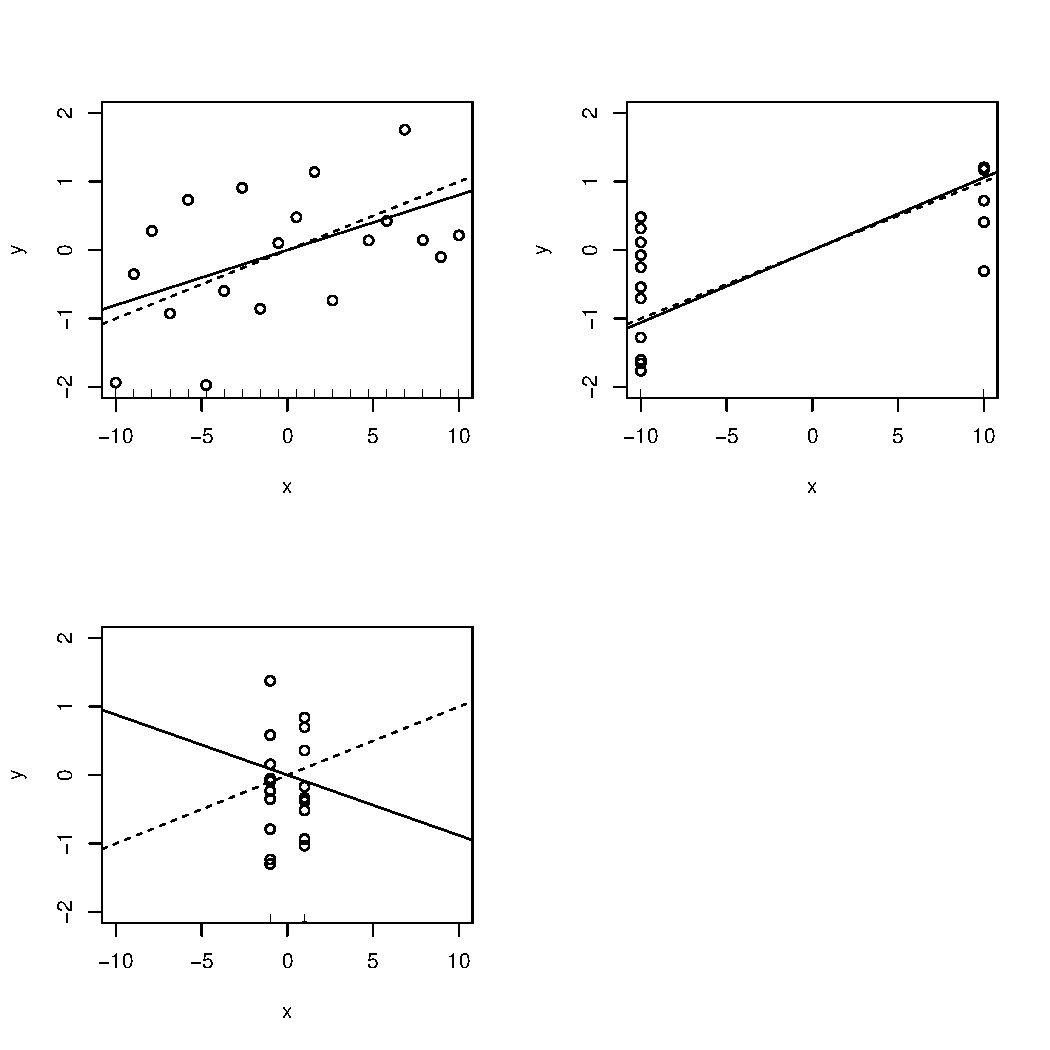
\includegraphics[height=0.3\textheight]{art/linear}
\caption[Design for Linear Models]{Design for linear regression. Different panels show different designs. True function as a dashed line. Estimated function as a full line.}
\label{fig:design_linear}
\end{figure}
\end{example}





\begin{example}[Design for non linear regression]
\label{eg:design_non_linear}
Figure~\ref{fig:design_nonlinear} demonstrates the effect of the different location of the sampling points ($x$) on the quality of the estimated regression line, in a \textbf{nonlinear} model.
The figure is non conclusive as to the best design, but it may seem that unlike the linear case (Example~\ref{eg:design_linear}) optimality is achieved in some non trivial sampling scheme.
\begin{figure}[ht]
\centering
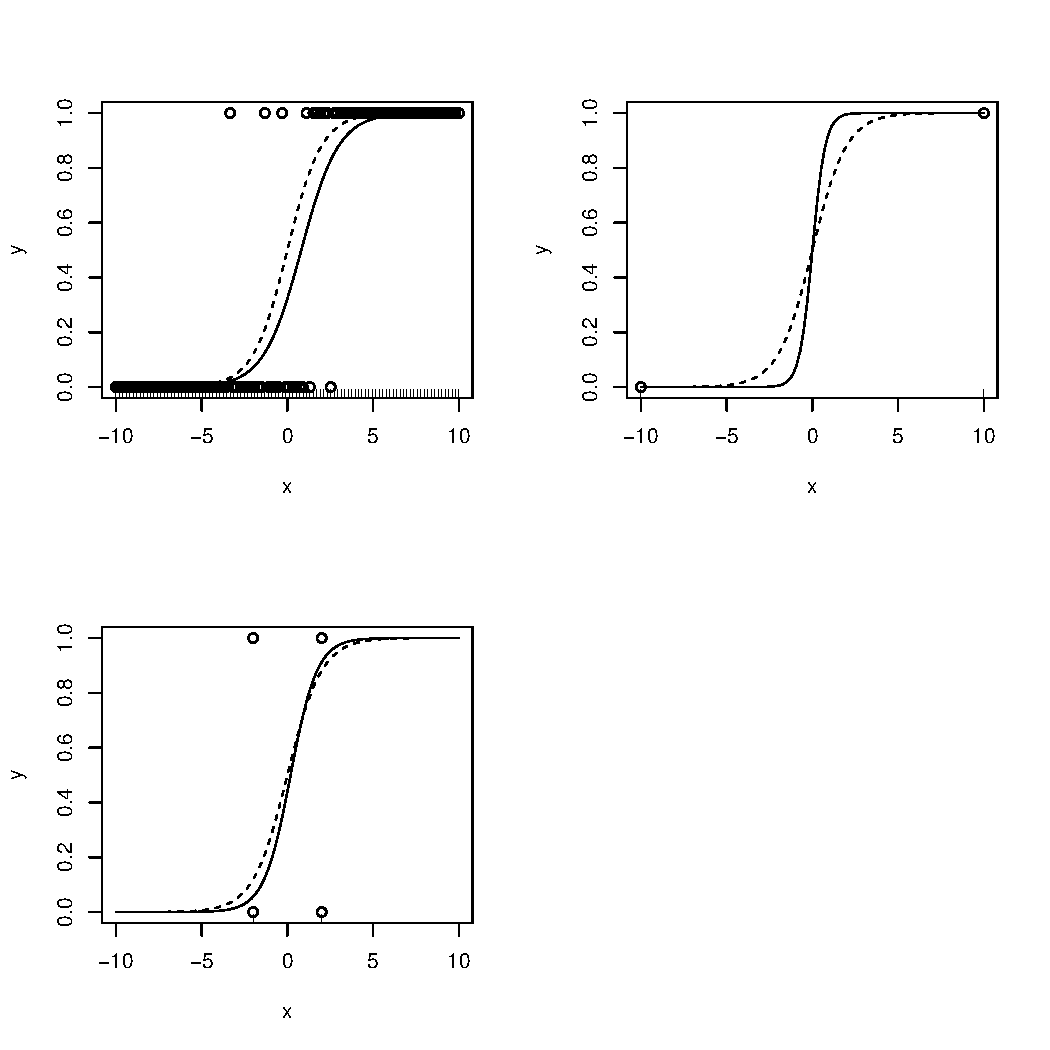
\includegraphics[height=0.3\textheight]{art/nonlinear}
\caption[Design for Non Linear Models]{Design for non linear regression. Different panels show different designs. True function as a dashed line. Estimated function as a full line.}
\label{fig:design_nonlinear}
\end{figure}
\end{example}





Now are some facts that are supported by the previous examples:
\begin{enumerate}
\item The idea of ``balancing'' as a design criterion is very useful with discrete factors, but limited with continuous factors. 
\item The optimal design may depend on the unknown generative model. Luckily, for linear models, this is not the case, and an optimal design will be so for all values of the generative parameter.
\end{enumerate}



\subsection{Space Filling Design}
\label{sec:space_filling}
The most natural of designs, which is particularly suitable when we have no a-priori assumption on the functional relation between the (continuous) factors, $f:x \mapsto y$,  and the response is known as a \emph{space filling design}.
As the name suggests, in a space filling design we aim at filling the factor space. Lacking any a-priori information, the filling will typically be as uniform as possible. 
We note however, that once information on $f$ is made available, then a space filling design is typically sub optimal (see Example~\ref{eg:design_linear}).

\begin{extra}[Space Filling and Hashing]
If you are familiar with the idea of \emph{hashing functions}, then you may see the similarity between space filling and the \emph{uniformity} property of hash functions. 
For a more rigorous discussion, see \cite{hill_first_1986}.
\end{extra}



\subsection{Covariance Optimality}
We have already noted the the optimality of the design depends on the data generating process.
In this section it is made obvious that optimality will also depend on the analysis method we choose.

When estimating the effect of a single continuous factor, we would like a design that gives us the most information per observation. This is the same as minimizing the variance of the estimator: $\min \{Var(\hat{\beta})\}$.

When generalizing to several continuous factors, with several effect, matters are more subtle.
This is because, having several parameters, we may consider several target criteria such as
minimal average variance, or minimal worst-case variance.
Matters further complicate when effect estimates are correlated, as will be promptly explained. 


\begin{definition}[Error Covariance Matrix]
For a $p$-vector of effects $\beta$, we define the $p \times p$ \emph{error covariance} matrix $M(\hat{\beta},\beta)$ to be 
\begin{align}
	M(\hat{\beta},\beta)_{i,j}:= \expect{(\hat{\beta}_i-\beta_i)((\hat{\beta}_j-\beta_j))}  
\end{align}
\end{definition}
Denoting $M=M(\hat{\beta},\beta)$, we readily note that for unbiased $\hat{\beta}$, then the diagonal of $M$ is simply the variances of $\hat{\beta}$, and the off-diagonal are the covariances. 
We also remark that if $p=1$, then $M$ is merely the scalar variance. 

We now try to generalize the idea of ``minimal variance'' to the multivariate case. 

\begin{definition}[A-Optimality]
	A design is said to be \emph{A optimal} if it minimizes the trace of $M$.
\end{definition}
A-optimality has an intuitive interpretation: since the average variance is proportional to the trace, then A-optimality is actually minimizing the average variance over effects.

Alas, A-optimality does not account for covariances. 
In an extreme scenario, if we have several copies of the same variable, the more copies we have, the more importance that variable will be given by A-optimality.
The most popular optimality criterion is known as \emph{D-optimality}, and does not suffer from this phenomenon.

\begin{definition}[D-Optimality]
	A design is said to be \emph{D optimal} if it minimizes the determinant of $M$.
\end{definition}
If you are familiar with the geometrical interpretation of the determinant, this definition may not surprise you. 
If not, then one way to think of D-optimality is via confidence regions.
D-optimality has the property that in the multivariate Gaussian case, a D-optimal design will return confidence regions for $\beta$ with smallest volume. 


\begin{extra}[Other Optimality Criteria]
There are as many optimality criteria as there are matrix norms. 
For a more detailed review, see \cite{wikipedia_optimal_2015}.
\end{extra}

The non-linear model example (\ref{eg:design_non_linear}) suggests that the optimal design may depend on the underlying (unknown) effect $\beta$. 
This is obviously bad news since if we had knowledge of $\beta$, we would not need an experiment to estimate it. 
There are, however, some good news.
First, for linear models and least-squares estimate, then $M$ will not depend\footnote{This is known as the \emph{equivariant in law} property.} on $\beta$, and neither will the optimal design. 
Second, when $M$ does depend on $\beta$, we will simply do some initial small experiment, and then optimize the design based on initial results. 



\section{Sequential Designs}
\label{sec:sequantial}
% Mark Vandelmeulenbruke

Consider a clinical trial with a treatment and control group.
Now assume the medicine being tested is a miracle cure with immediate improvement. 
Do we really need to keep administering placebos to the control group, just because that was the initial experimental design?
This is where sequential designs come in.
Interestingly, the initial application of a sequential design was not in drug testing, but rather in a military context \citep{wald_sequential_1945}.

The problem with sequential testing, is the \emph{type-I error inflation}, which is simply a \emph{multiplicity problem}. \marginnote{Multiplicity}
To see this, think about an endless sequential experiment. Also assume the null hypothesis is true. 
Can we agree that a regular (non sequential) experiment will not reject $H_0$? 
Can we also agree that a sequential experiment will necessarily reject $H_0$ at some stage?

In it simplest version, a sequential design allows early stopping for rejection of the null, or for futility (non-rejection). 
In more elaborate schemes then not only is early stopping allowed, but also the redesign of the experiment. 
This is known as \emph{adaptive design}. The crux, as usual, is not inflating the type-I error, or introducing bias, by redesigning.\marginnote{Adaptive Design}


\begin{extra}[Active Learning]
In the machine learning literature, the idea of adaptive design of experiments is known as \emph{active learning}, where the emphasis is less on adaptive-testing, but rather on adaptive-estimation.
\end{extra}


\section{AB Testing}
[TODO]




\section{Computer Experiments}
% no randomness
% space filling parameter choices for simulation
\begin{example}[Designing Wings]
\label{eg:wings}
Consider the problem of designing an air-craft's wing.
We would like to know how the wing's attributes, i.e., factors, govern its lift.
We could obviously conduct real-life experiments by varying the wing's attributes, building the wing, flying the air-plane, and recording results. 
Needless to say how expensive this process is.
It is much more reasonable to program the differential equations that govern the lift to a computer, fix several factors values, and solve the equations.
This is what \emph{computer experiments} are all about. 
\end{example}


The wind design example (\ref{eg:wings}) demonstrates the following points:
\begin{enumerate}
\item Computer experiments are essentially numerical solutions to complicated systems of equations.
\item Because solutions take a lot of time, only a small finite set of values may be evaluated. 
\item The ``response'' to each treatment, is deterministic. 
\item The problem of interest is in reconstructing the response at non measured factor values, so that optimal values may be identified. 
\end{enumerate}
It is thus not uncommon to call upon DOE theory for choosing the factor combinations to be experimented with. Space filling designs (Sec.~\ref{sec:space_filling}) being a particularly prevalent choice. 
The analysis of computer experiment is very different than real-life experiment since we have no noise component. 
See \cite{sacks_design_1989} or \cite{santner_design_2013} for further details. 



\section{Bibliographic Notes}
% Cox and Reid
% Penn State Stats 503: https://onlinecourses.science.psu.edu/stat503/node/1

% % % % Acceptance Sampling 
\chapter{Acceptance Sampling}
\chaptermark{Acceptance}

% AQL
% LTPD
% RQL
% LQL
% Type A and Type B RO curves.

We can improve quality (read- conformance to specification) by introducing an inspection stage in our process.
Clearly, a full inspection is time consuming. 
It may also be destructive (you don't want to re-package ice-cream after checking its texture \dots).
No-inspection may be appropriate if you don't particularly care about your brand, or if production has very high capability indices.
A reasonable, intermediate approach, is a partial random inspection, known as \emph{acceptance sampling}.
As the name suggests, in acceptance sampling, one samples, then checks, then accepts (or not).

Acceptance sampling can be seen as a control chart monitoring that triggers active intervention in the production. As such ,it is a crude type of \emph{engineering control} (Sec.~\ref{sec:terminology_statistical}).
The intervention is obvious. The monitoring is based on some continuous (variable) or discrete (attribute) of a sample of units from a \emph{batch}, \aka, a \emph{lot}.
Seen as a feedback control, it is not surprising that when designing an acceptance sampling scheme, we have similar decisions as when designing a control chart:
\begin{enumerate}
\item What is a batch? Just like choosing the sampling frequency in a Shewart chart. 
We would like homogenous batches, i.e., with low inner variability. A box, a shipment, a day's production, are typical batches. 
\item Within batch sampling scheme: just like rational grouping in Shewart chart. Typical approaches include \emph{single sampling plans}, \emph{double}, \emph{multiple}, and \emph{sequential sampling plans}.
This can be seen as the design of an experiment to be performed on each batch.
\item How many units? Just like choosing the sample size in a Shewart chart.
\item Decision cutoff: Just like setting control limits in a Shewart chart. 
\end{enumerate}
We can readily see that the design of an acceptance sampling scheme is very similar to the design of a control chart. 
We may construct an full blown economical optimization problem to design the sampling, as we did in Section~\ref{sec:economical_considerations}. Just like control charts, however, it is more common to design sampling schemes using ``first-order'' power considerations. 
For this reason, the \emph{power function} will play a crucial role.

\section{Acceptance Sampling Terminology}
Adapted from \cite{natrella_nist/sematech_2010}.
\begin{description}
\item [LASP] A \emph{lot acceptance sampling plan}, ultimately, a statistical test at the end of which we either accept a batch. In this text we typically use the \emph{batch acceptance sampling scheme} for the same purpose. 
\item [AQL] The \emph{acceptable quality level}, or \emph{acceptable quality limit}, is the highest proportion of defects acceptable to the producer. 
\item [LTPD] The \emph{lot tolerance percent defective} is the highest proportion of defects acceptable to the consumer. Clearly, $AQL<LTPD$. LTPD is also known as \emph{rejectable quality level} (RQL), and \emph{ limiting quality level} (LQL). 
\item [OC Curve] The \emph{operating characteristic curve} is the power function of an LSAP.
\item [Type-A and Type-B OC Curves] A \emph{Type-A OC curve} is one computed assuming sampling from batches is done without replacement. Conversely, a \emph{Type-B OC curve} is computed assuming sampling with replacement.
\item [Producer's Risk] The \emph{producer's risk} is throwing away good batches. Formally, this is the probability of rejecting a batch with less than AQL defects. We consider there type-I errors.
\item [Consumer's Risk] The \emph{consumer's risk} is accepting bad batches. Formally, this is the probability of accepting a batch with more than LTPD defects. We consider there type-II errors.
\item [Rectifying Inspection] An LASP where lots are not rejected but rather rectified. 
\item [AOQ] The \emph{average outgoing quality}, as the name suggests, is the average proportion of defects after a rectifying inspection has been introduced in the process. 
\item [AOQL] The \emph{average outgoing quality level} is the (unknown) defect proportion that would return the worst AOQ after a rectifying inspection.
\item [ATI] The \emph{average total inspection}, as the name suggests, is the average number of units inspected in a batch.
\end{description}



\section{Single Sampling Scheme}
In the simplest LASP we base our decisions on a single random sample from each batch.
This obviously facilitates the statistical analysis of the properties of this LASP.

When sampling $n$ units from a batch with a proportion of $p$ defects, then the number of defects $\x \sim Binom(n,p)$.
If we reject a batch when more than $c$ defects are found, then the power function of a type-B LASP is given by
\begin{align}
\label{eq:power_accpet}
	\pi_{n,c}(p)=P(\x \geq c)= \sum_{k=c}^n \binom{n}{k} p^k (1-p)^{1-k} .
\end{align}
Eq.(\ref{eq:power_accpet}) may be evaluated manually, or with the \rcode{pbinom()} \R function. 

Just like any other hypothesis test, it is common practice to set $n,c$ so that control both the consumer's risk ($\beta=1-\pi$) and the producer's risk ($\alpha$).





% % % % Reliability
\chapter{Reliability Analysis}
\chaptermark{Reliability}

The attempt to define the difference between \emph{reliability} and \emph{quality} will certainly fail given the intentional ambiguity in our definition of \emph{quality} (Chapter~\ref{sec:introduction}).
For our purposes, however, this terminological matter will not matter, since we will simply define reliability analysis to be the analysis of the \emph{time} to \emph{failure}.
We will also assume that ``time'' and ``failure'' are well defined and agreed upon.

We intuitively understand ``more reliable'' to mean ``lasts longer''. 
We should also consider, however, the case of a product that is designed to fail after some time, thus forcing the consumer to buy a new one. 
Some may say that a major hi-tech company named after a fruit employs this practice. 
Be it true or not, I hope we can agree that good knowledge of your product's life expectancy is a desirable. 

Reliability analysis involves the study of a probabilistic property of our product- its \emph{survival}.
Any probabilistic model will require calibration to reality via data. 
This chapter thus introduces both the probability calculus typically used for reliability analysis, and some statistical considerations involved when calibrating these models.



\section{Probabilistic Analysis}




\subsection{A Static View}

Let $\x_j \in \set{0,1}, j=1,\dots,p$ denote the state of the $j$'th component of a system, and $x=(x_1,\dots,x_p)$.

\begin{definition}[Structure Function]
The \emph{structure function}, $\struct=\struct(x):x \mapsto \set{0,1}$, is an indicator function of the state of the system. A failure indicated by $0$. 
\end{definition}

\begin{remark}[$\Phi$]
We apologize to the reader for using $\Phi$ to denote both the $\gauss{0,1}$ CDF, and the structure function.
We do so to stay in accordance with reliability literature, and since no collisions are created in this chapter by doing so.
\end{remark}

\begin{definition}[Series System]
A \emph{series system}, or \emph{serial system}, is one where all components need to function for the system to function: $$\struct(x)=\prod_{j=1}^{p}x_j.$$
\end{definition}
A reliability diagram of a series system is given in Figure~\ref{fig:series_system}.
\begin{figure}[ht]
\centering
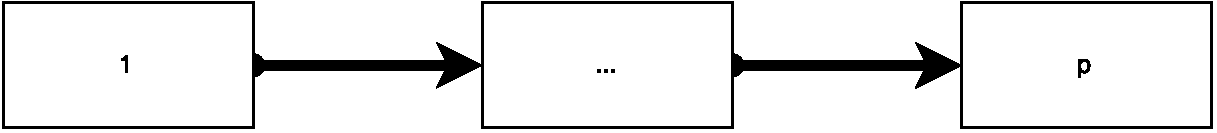
\includegraphics[width=0.5\linewidth]{art/series_system}
\caption{Series system.}
\label{fig:series_system}
\end{figure}


\begin{definition}[Parallel System]
A \emph{parallel system} is one where all components need to fail for the system to fail:
$$\struct(x)=1-\prod_{j=1}^{p} (1-x_j)= \coprod_{j=1}^p x_j.$$
\end{definition}
A reliability diagram of a parallel system is given in Figure~\ref{fig:parallel_system}.
\begin{figure}[ht]
\centering
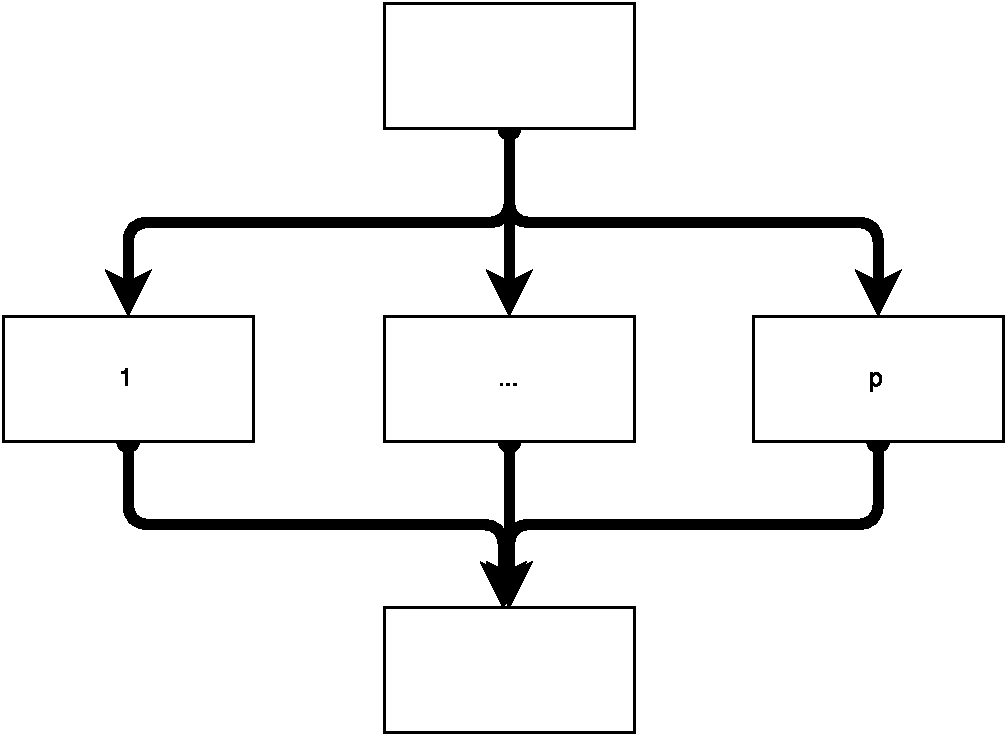
\includegraphics[width=0.5\linewidth]{art/parallel_system}
\caption{Parallel system.}
\label{fig:parallel_system}
\end{figure}





\begin{definition}[k-out-of-p System]
A \emph{k-out-of-p} system is one where at least $k$ components need to function for the system to function:
$$\struct(x)=\indicator{\sum_{j=1}^{p} x_j \geq k}.$$
\end{definition}
A reliability diagram of a k-out-of-p system is not provided, since it is not very friendly. Try thinking of a 2-out-of-3 system to see why.




\begin{tcolorbox}
\paragraph{My mistake!}
The previous definition is different than the one I gave in class. 
I initially defined it via failing components, while now it is defined via functioning components.
Please note this when comparing your notes to mine.
\end{tcolorbox}




\begin{definition}[Monotone System]
A system is said to be \emph{monotone} if $\struct(x_1,\dots,x_p)$ is non decreasing in all components.
\end{definition}
The definition of monotonicity captures the idea that you cannot improve a system's state by breaking components.
This seems rather natural (I am still looking for a counter example).






\begin{definition}[Reliability]
We define the \emph{reliabity of component $j$} to be $$p_j:= P(\x_j=1),$$ 
and  the \emph{reliability of the system} 
$$ S_\struct = S_{\struct(x)}:=P(\struct(x)=1).$$
\end{definition}


\begin{example}[Reliability of a series system]
For $\Phi(x)$ a series system, assuming independent components, we have
$$ S_\struct= \prod_{j=1}^{p} p_j.$$
\end{example}


\begin{example}[Reliability of a parallel system]
For $\Phi(x)$ a parallel system, assuming independent components, we have
$$ S_\struct= 1-\prod_{j=1}^{p} (1-p_j)= \coprod_{j=1}^p p_j. $$
\end{example}


\begin{example}[Reliability of a k-out-of-p system]
For $\Phi(x)$ a k-out-of-p system, assuming independent components with equal reliability ($p_i=p_0$), we have
$$ S_\struct= \sum_{i=k}^{p} \binom{p}{i} p_0^i (1-p_0)^{p-i} .$$
\end{example}



\subsubsection{State enumeration method}
To compute the reliability of more complex structures, the brute-force approach is the \emph{state enumeration method}. 
This method simply relies on summation of the probabilities of the states for which the system functions.
$$ S_\struct= \sum_{x} \Phi(x) P(\x=x).$$


\subsubsection{Factoring method}
The \emph{factoring method}, \aka \emph{pivot-decomposition method}, relies on two ingredients: 
(a) conditioning on the state of some components greatly simplifies the structure, and
(b) the total probability argument.
Combining the two we have:
$$ S_\struct= p_j  S_{\struct|x_j=1} + (1-p_j) S_{\struct|x_j=0}   ,$$
where $S_{\struct|x_j=1}$ denotes the reliability of the structure $\Phi$ conditional on $x_j=1$.
The following example demonstrates the power of the factoring method.

\begin{example}[Bridge Structure]
\label{eg:bridge}
Consider structure in Figure~\ref{fig:bridge}.
To compute the reliability, we will call upon the factoring method while conditioning on the state of component $3$:
$$ S_\struct= p_3  S_{\struct|x_3=1} + (1-p_3) S_{\struct|x_3=0}   .$$
Now note that when $x_3=1$ then we have a series structure of parallel structures, while when $x_3=0$ we have a parallel structure of series structures.:
\begin{align*}
	S_{\struct|x_3=1} &= (p_1 \coprod p_2) (p_4 \coprod p_5),\\
	S_{\struct|x_3=0} &=  p_1 p_4 \coprod p_2 p_5,
\end{align*}
so that 
$$ 	
	S_\struct = p_3  (p_1 \coprod p_2) (p_4 \coprod p_5) + (1-p_3) (p_1 p_4 \coprod p_2 p_5).
$$
\begin{figure}[ht]
\centering
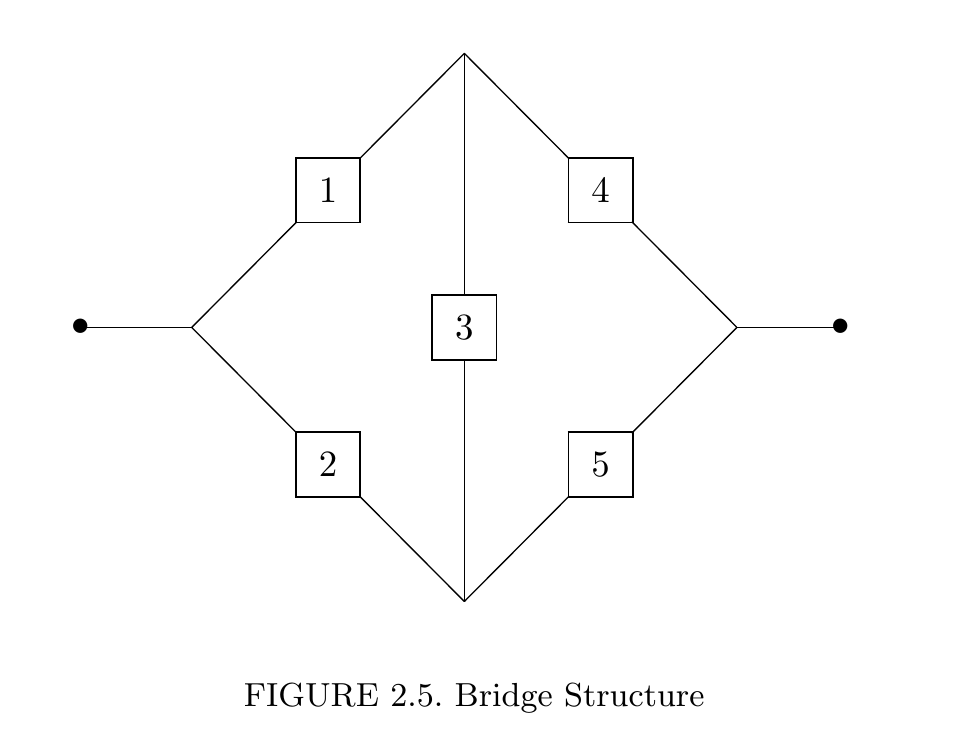
\includegraphics[width=0.5\linewidth]{art/bridge}
\caption{Structure of a bridge system. Source: \cite[Fig.2.5]{aven_stochastic_1999}}
\label{fig:bridge}
\end{figure}
\end{example}
Example~\ref{eg:bridge} demonstrates a single application of the factoring method. Clearly, it can be applied recursively for more complicated systems.

The example also demonstrates a more general principle. Namely, that redundancy is preferable at the component level, and not at the system's level.
Put differently- when designing a backup, and the resources allow a fill copy of the original system, we are better of by designing a component-wise backup, than a single backup system.
Put formally:
\begin{theorem}[Component-wise redundancy]
For a monotone structure $\Phi$, 
\begin{align}
	S_{\struct(x \coprod y)} \geq S_{\struct(x)} \coprod S_{\struct(y)}
\end{align}
where $x \coprod y$ denotes a component-wise backup: $(x_1 \coprod y_1,\dots,x_p \coprod y_p)$.
\end{theorem}



\begin{extra}[Reliability analysis of complex systems]
Except for simple systems, of the type we presented, the computation of the reliability of a complex system may be a formidable task. 
For complicated real-life systems, \emph{min-cut--max-flow} algorithms, or \emph{inclusion-exclusion} type algorithms are employed. 
For more details, see \cite{aven_stochastic_1999}.
\end{extra}









\subsubsection{Reliability Importance Measures}
\begin{quotation}
The Strength Of The Chain Is In The Weakest Link.
\end{quotation}
This is obviously a profound observation in reliability analysis.
In order to identify the weakest link we require some measure of reliability importance.


\begin{definition}[Improvement potential]
The \emph{improvement potential} is defined as the change in a system's reliability, if we could force a component to function indefinitely.
Formally, we denote $\Phi^{(j)}$ to be a system where component $j$ cannot fail. 
We then define the improvement potential with respect to component $j$ to be 
\begin{align}
	I_j :=S_{\Phi^{(j)}}-S_{\Phi}.
\end{align}
\end{definition}



\begin{definition}[Birenbaum's measure]
\emph{Birenbaum's measure} is defined as the change in a system's reliability, if we infinitesimally improve the reliability of component $j$.
Formally 
\begin{align}
	I_j: =\frac{\partial}{\partial p_j} S_{\Phi}.
\end{align}
\end{definition}


Clearly any such importance measure, once computed, may serve to decide which component should be treated to improve reliability.







\subsection{A Time Dynamic View}
The reliability of each component ($p_j$), typically changes in time, and so does the reliability of the whole system.
In the following, $\T$ will typically stand for the time to malfunction. It is thus assumed to be \textbf{continuous} and \textbf{non-negative}.


\begin{definition}[CDF]
The cumulative distribution function (CDF) of a random variable $\T$ at a point $t$  is given by
\begin{align}
	\cdf{\T}{t}:= P(\T<t).
\end{align}
\end{definition}

\begin{definition}[PDF]
The probability density function (PDF) of a continuous random variable $\T$ at a point $t$ is given by 
\begin{align}
	\pdf{\T}{t}:= \frac{\partial}{\partial t}\cdf{\T}{t}.
\end{align}
\end{definition}


\begin{definition}[Survival Function]
The survival function of a random variable $\T$ at a point $t$ is given by 
\begin{align}
	\survive{\T}{t}:= P(\T>t)=1-\cdf{\T}{t}.
\end{align}
\end{definition}
By definition, it follows that if $\T_j$ is the time to failure of component $j$, then $p_j(t)=\survive{\T_j}{t}$.
If $\T_\struct$ is the time to failure of a system $\Phi$, then we may write $S_\struct(t)=\survive{\T_\struct}{t}$.


\begin{example}[Survival of a series system]
For a series system $\struct$, the reliability of the system at time $t$ is given by $$\survive{\Phi}{t}=\prod_{j=1}^{p} p_j(t).$$
\end{example}


\begin{example}[Survival of a parallel system]
For a parallel system $\struct$, the reliability of the system at time $t$ is given by $$\survive{\Phi}{t}=1- \prod_{j=1}^{p} (1-p_j(t))= \coprod_{j=1}^p p_j(t).$$
\end{example}





Another way to present a distribution, no less informative than the previous ones, is by the \emph{hazard function}, which is the ``probability of surviving just another instant''.
\begin{definition}[Failure Rate]
The \emph{hazard function}, or \emph{failure rate}, of a random variable $\T$ at a point $t$ is given by \marginnote{Hazard Function}
\begin{align}
	\hazard{\T}{t} &:= \lim_{dt\to 0}\frac{P( \T \in [t,t+dt)|\T \geq t )}{dt} \label{eq:hazard}\\
	&= \frac{\pdf{\T}{t}}{\survive{\T}{t}} \\
	&= \frac{\partial}{\partial t}\log \survive{\T}{t}.
\end{align}
\end{definition}





\begin{definition}[Cumulative Risk]
The \emph{cumulative hazard}, \aka the \emph{cumulative risk}, of a random variable $\T$ at a point $t$ is given by \marginnote{Cumulative Hazrd}
\begin{align}
	\cuhazard{\T}{t} &:= \int_{0}^{t}\hazard{\T}{t} \\
	\Rightarrow \survive{\T}{t} &= \exp(-\cuhazard{\T}{t}). \label{eq:cumhazrd}
\end{align}
\end{definition}
Eq.(\ref{eq:cumhazrd}) readily shows that a distribution is well defined by its hazards.



\begin{theorem}[Failure rate of a series system]
\label{thm:ifr_closure}
The failure rate of a series system of independent components $\Phi$ is given by the sum of the failure rates of its components
\begin{align}
	\hazard{\Phi}{t}= \sum_{j=1}^{p} \hazard{\T_j}{t}
\end{align}
\end{theorem}
The proof is immediate using the cumulative risk.
The failure rate of a parallel system, does not admit such a nice closed form as we will soon see in Example~\ref{eg:failure_parallel}.




\begin{example}[Exponential Hazard]
The simplest distribution when discussing hazards is the exponential.
Recalling the for non-negative $t$:
\begin{align}
	\pdf{\T}{t}= \lambda \exp(-\lambda t), \\
	\cdf{\T}{t}= 1-\exp(-\lambda t),
\end{align}
so that 
\begin{align}
	\survive{\T}{t} &= \exp(-\lambda t), \\
	\hazard{\T}{t} &= \lambda.
\end{align}
\end{example}
The exponential is the only distribution with constant hazard which makes it very easy to analyze.
The constant hazard is due to the \emph{memoryless} property. Look at Eq.(\ref{eq:hazard}) and think why.

% [HW: prove that memory less is sufficient]


\begin{example}[Failure rate of a series of exponential components]
The failure rate of a series system $\Phi$, of $p$ independent components each with exponentially distributed failure times, is simply 
\begin{align}
	\hazard{\Phi}{t}= \sum_{j=1}^{p} \lambda_j, \forall t \geq 0
\end{align}
where $\lambda_j=\lambda_j(t)$ is the rate of each component.
\end{example}
This is obviously the simplest system possible for reliability analysis, which stems from the fact that a minimum of exponentials is exponential with the sum of rates.



The following example, seemingly very simple, provides tremendous insight into the complexities of reliability analysis.
\begin{example}[Failure rate of a two exponential-component parallel-system]
\label{eg:failure_parallel}
Consider a system of two independent, parallel, exponential components, with failure times $\T_j\sim \exp(\lambda_j); j=1,2$.
The failure rate is given by
\begin{align}
	\hazard{\Phi}{t}=
	\frac
	{\exppdf{\lambda_1}{t} + \exppdf{\lambda_2}{t}  - \exppdf{(\lambda_1+ \lambda_2)}{t}}
	{\expcdf{\lambda_1}{t} + \expcdf{\lambda_2}{t} - \expcdf{(\lambda_1+ \lambda_2)}{t}}
\end{align}
\end{example}
Why is Example~\ref{eg:failure_parallel} so important?
Because it demonstrates that even in a simple system, with the simplest components, the reliability is not so simple to compute (as a function of the components' reliability). 
Indeed, even though the component-wise hazards are fixed in time, the system's hazard is not fixed, and not even monotone in time (Figure~\ref{fig:hazard_non_monotone}). 


\begin{figure}[ht]
\centering
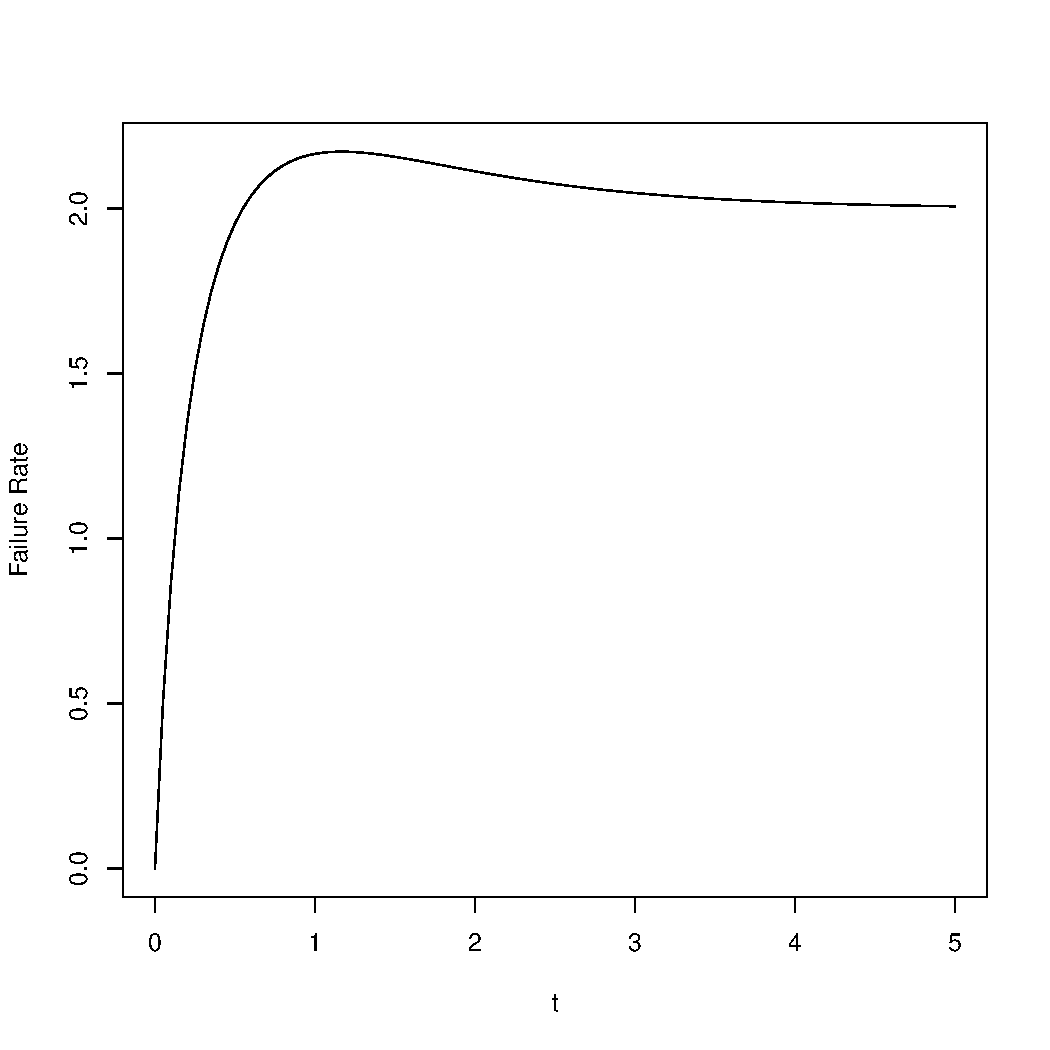
\includegraphics[width=0.5\linewidth]{art/hazard}
\caption{Failure rate of the parallel exponential component system.}
\label{fig:hazard_non_monotone}
\end{figure}





\begin{example}[Weibull Hazard]
The Weibull distribution is very common in reliability analysis since it is tractable generalization of the exponential distribution with many nice properties. It can be constructed by 
$\T := \lambda \U^{1/k}$, where $\U \sim \exp(1)$. 
This implies that for non negative $t$:
\begin{align}
	\pdf{\T}{t} &= \frac{k}{\lambda}\left(\frac{\T}{\lambda} \right)^{k-1} e^{-(\T/\lambda)^k}, \\
	\cdf{\T}{t} &= 1 - e^{-(\T/\lambda)^k},
\end{align}
so that 
\begin{align}
	\survive{\T}{t} &= \exp \left(-\frac{\T}{\lambda} \right)^k, \\
	\hazard{\T}{t} &= \frac{k}{\lambda} \left(\frac{\T}{\lambda} \right)^{k-1} .
\end{align}
\end{example}
Elementary analysis shows that the hazard function of the Weibull may be increasing or decreasing in time ($\T$), depending on $k$, but it is always monotone.




\begin{example}[Empirical risk rates]
When examining empirical risk rates of true devices, we almost always notice a \emph{bathtub} structure, such as in Figure~\ref{fig:bathtub}.\marginnote{Bathtub}
This shape captures the idea that products tend to fail more when they are brand new, or as they are very old, while their failure rates are fairly stable in the ``mid-life''.
In this text, we will not be providing a particular distribution which has this property. 
We refer the reader to \cite{nadarajah_bathtub-shaped_2008} for examples of distributions which have the bathtub property.
\end{example}


\begin{figure}[ht]
\centering
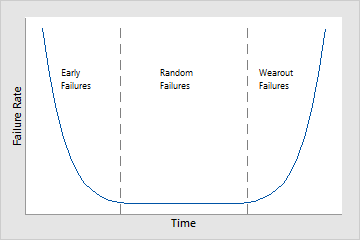
\includegraphics[width=0.5\linewidth]{art/bathtub_curve}
\caption[Bathtub empirical hazard curve]{Bathtub curve of empirical failure rates. \newline
\url{http://support.minitab.com/en-us/minitab/17/topic-library/modeling-statistics/reliability/distributions-in-reliability-analysis/hazard-functions/}}
\label{fig:bathtub}
\end{figure}




\subsubsection{Aging}
The idea of \emph{aging} is that failure rate may vary over time. It is an important concept in reliability, as demonstrated by the empirical bathtub failure rate (Figure~\ref{fig:bathtub}).
Instead of checking if a particular textbook distribution has some ageing property, we instead analyze classes of distributions with the desired notion of ageing.
Our goal will ultimately be to understand the ageing of a whole system, as a function of the ageing of its components.

\begin{definition}[IFR]
We call a failure time distribution to be in the \emph{increasing failure rate} (IFR) ageing class, if it has a non decreasing failure rate.
\end{definition}


\begin{definition}[IFRA]
We call a failure time distribution to be in the \emph{increasing failure rate average} (IFRA) ageing class, if 
$\cuhazard{\T}{t}/t$ is non decreasing in $t$.
\end{definition}

\begin{definition}[NBU]
We call a failure time distribution to be in the \emph{new better then used} (NBU) ageing class, if 
$\survive{\T}{t_1+t_2} \leq \survive{\T}{t_2} \survive{\T}{t_1}$.
\end{definition}

\begin{definition}[NBUE]
Define the \emph{expected residual life}, $\mu(t)$, to be 
$$\mu(t):= \expect{\T-t|\T>t}.$$
\marginnote{Expected Residual Life}
We call a failure time distribution to be in the \emph{new better then used in expectation} (NBUE) ageing class, if 
$\mu(t) \leq \mu(0)$.
\end{definition}


\begin{theorem}
$IFR \Rightarrow IFRA \Rightarrow NBU \Rightarrow NBUE. $
\end{theorem}


The following theorem states a relation between the ageing properties of particular components, and that of the whole system. In particular it states that for the (very wide) class of monotone systems, then the IFRA property is conserved. 
This should be contrasted with the IFR property, which is not conserved, as demonstrated by the parallel system in  Example~\ref{eg:failure_parallel}.
\begin{theorem}[IFRA closure theorem]
\label{thm:ifra_closure}
If the independent components of a monotone system are IFRA, then so is the whole system.
\end{theorem}


Series systems are a extremely small and particular subset of monotone systems.
It does provide, however, an example of systems where not only IFRA is preserved, but also the stronger IFR.
The following corollary follows immediately from Theorem~\ref{thm:ifr_closure} and the fact that a sum of monotone functions is monotone.
\begin{cor}[IFR closure for series systems]
\label{cor:ifr_series}
A series system of independent IFR components is IFR.
\end{cor}




Now consider a two-component system, where one component kicks-in when the first fails.
We will call this an \emph{offline backup}.\marginnote{Offline Backup}
The survival times of the components in an offline backup system are clearly dependent. 
It turns out that for such a system of IFR components, does conserve the IFR property, as seen in the following theorem.
\begin{theorem}[Convolution of IFR]
\label{thm:ifr_convolution}
For two independent random variables, $\x$ and $\y$, both in the IFR ageing class, then so is $\x+\y$.
\end{theorem}
The theorem is called the convolution theorem, because the distribution of a sum of independent random variables, is the convolution of their distributions.


\begin{extra}[IFR and log-concave]
The IFR requirement, is essentially the same as log-concavity of the density function.
This immediately implies many properties of the class, including the convolution theorem above.
See \cite{bagnoli_log-concave_2005}.
\end{extra}

\begin{example}[IFR of Gamma]
The Gamma (and thus the Erlang) distribution is in the IFR aging class, since it is the sum of exponentials, each IFR.
\end{example}

\begin{example}[Series system of offline backups]
What can we say about the ageing class of a series systems of offline backup systems? 
It turns out that if the components are IFR, then so will the whole system.
This is immediate from Corollary~\ref{cor:ifr_series} and Theorem~\ref{thm:ifr_convolution}.
\end{example}






\section{Statistical Analysis}
The probabilistic analysis of the previous section is great fun and all, but like any probabilistic problem, is has to be calibrated to real life. 
This is where data, and statistics come in.
Indeed, given any particular probabilistic model, we may write the likelihood problem, and call upon maximum likelihood principles for estimation.

Failure data and models introduces particular statistical challenges:
\begin{description}
\item [Identifiability] It is typically hard, if not impossible, to estimate the reliability of particular components, from the reliability of the whole system. 
\item [Censoring] A major concern with reliability data, is that in any finite length experiment, some events will just not have happened yet; their failure time will thus be \emph{censored}. Ironically- the more reliable a component, the less data we will have to estimate its reliability. 
\item [Lab versus real-life conditions] Reliable components take very long time to fail. We will thus extrapolate from harsh lab conditions to real-life operating conditions. This requires the introduction of covariates. 
\item [Failure Distribution] like any statistical model, we will need to commit to some failure time sampling distribution.
\end{description}


\subsection{Identifiability}

\begin{example}[Likelihood estimation of a series system]
\label{eg:likelihood_of_failures}
Assume a series system $\Phi$ with $p$ independent, exponential components with rates $(\lambda_1,\dots,\lambda_p)$.
We have $n$ observations on the failure times of the system $t_1,\dots,t_n$.
How can we estimate the failure rates?
To use a likelihood approach, we need the data's sampling distribution.
Denoting the failure time of the $j$'th component of the $i$th device with $\T_{i,j}$, we have that $\T_{i,j}\sim \exp(\lambda_j)$ by assumption.
Since the system is serial, then $\T_i=\min_j(\T_{i,1},\dots,\T_{i,p})$.
By the properties of the exponential distribution $\T_i \sim \exp(\lambda)$, where $\lambda:=\sum_{j=1}^{p} \lambda_j$, as we have already seen with the failure rate. It follows that
$\pdf{\T_i}{t}=\lambda \exp(-\lambda t)$.
We may then write the likelihood function, maximize it with respect to $\lambda$ and discover, as we already know, that $$\hat{\lambda}=\frac{n}{\sum_{i=1}^{n} t_i}.$$
We are now left with the problem of recovering $(\lambda_1,\dots,\lambda_p)$ from $\lambda$. 
Can we do it? On the face of it- no. Which should not surprise us, since the mere knowledge of a device failure, is not very informative on the particular component that failed, which we would need to estimate $(\lambda_1,\dots,\lambda_p)$.
\end{example}

Example~\ref{eg:likelihood_of_failures} teaches us that unless further assumptions are introduced, the estimation of the component-wise failure rates requires information on the component-wise failure times. 





\subsection{Censored Events}
Consider several components being analyze for their reliability. 
Ironically, we actually want them to fail. If they do not, they do not convey information on their reliability.
In the event that a component has not failed, we clearly cannot register its failure time. Omitting this component from the sample will upward bias the estimated reliability.
These events are called \emph{censored} observations. 
There are several types of censoring which depend on the design of the study and the type of event recorded. 
They are all dealt with careful though on the sampling distribution of the data, and the probability of a censoring event. 

Design considerations:
\begin{description}
\item [Type I] occurs when the design is such that the sampling time is fixed a-priori. This implies that the number of failures (thus censoring) events is random. 
\item [Type II] occurs when the design is such that the number of failures (thus censoring) is fixed a-priori. This implies that the sampling duration is random.
\end{description}
If all we know on a censored event is that the actual lifetime is larger then the observation period, we call this a \emph{non-informative} censoring. 
Both designs will then lead to the same modelling of the censoring event, which is now described.

The likelihood function of non-censored events is given by
\begin{align}
	\lik_i=\density_\T(t_i)= \survive{\T}{t_i} \hazard{\T}{t_i},
\end{align}
and the likelihood of a censored event, under the \emph{non-informative} assumption, is given by 
\begin{align}
	\lik_i=\survive{\T}{t_i} .
\end{align}
Unifying the two cases assuming independent observations, using an indicator for censoring, $c_i$, and taking logs we have
\begin{align}
	\loglik &=\log \lik\\ 
	&= \log \prod_{i=1}^{n} \lik_i \\
	&= \log \prod_{i=1}^{n} \survive{\T}{t_i} \hazard{\T}{t_i}^{c_i} \\
	&= \sum_{i=1}^{n} [c_i \log \hazard{\T}{t_i} - \cuhazard{\T}{t_i}]. \label{eq:censored_likelihood}
\end{align}


\begin{example}[Censored exponential lifetimes]
Recalling that the failure rates of exponential lifetimes are fixed, we have that the likelihood of censored exponential lifetimes is given by 
$$
	\sum_{i=1}^{n} [c_i \log \lambda - \lambda t_i].
$$
The maximum likelihood estimator of $\lambda$ is thus
\begin{align}
	\estim{\lambda}= \frac{\sum c_i}{\sum t_i}. \label{eq:censored_ml}
\end{align}
Eq.(\ref{eq:censored_ml}) lends itself to a nice interpretation.
The nominator is the total number of failures.
The denominator is the total \emph{exposure time}. 
The estimated failure rate is thus the number of failures per unit of exposure time. 
\end{example}




\begin{extra}
The previous result is obvious is you consider failures as events which come as a Poisson process, which is implied from the exponential times assumption. 
The process is run for $\sum t_i$ time, and the total event count is $\sum c_i$. 
The trivial estimator for the rate of the process, is $\sum c_i/\sum t_i$.
\end{extra}






\subsection{Accelerated Life Models}
The \emph{accelerated life} model is very popular for very reliable components. This is because it may take forever to produce defect. We thus ``accelerate'' life, by testing under extreme conditions, and then scale back to the regular operating environments.

An accelerate life mode assumes that covariates rescale time. 
For instance, the lab may produce conditions where time advances ten times faster than in real-life operating conditions.
To introduce the model, we start with a simple two group example.
\begin{example}[Two group accelerated life]
Consider two groups indexed by a single dummy variable $x_i \in \set{0,1}$.
Assuming an accelerated life effect we have
$$
	\survive{x_i=1}{t}=\survive{x_i=0}{t/exp(\beta)}=\survive{x_i=0}{t/\gamma}, 
$$
where $\gamma$ is simply shorthand notation for $exp(\beta)$. 
If $\gamma=1/2$, this means that time for group $x_i=1$ advances twice as fast as for group $x_i=0$.
\end{example}

We now generalize the idea for multiple covariates.
If $\T_1$ is the time to failure under conditions $x_1$ , and $\T_2$ under conditions $x_2$. 
And the covariates' effects are such that $x_1' \beta=1$ and $x_2' \beta=\log \gamma$,  then 
\begin{align}
\label{eq:accelerated_life}
	\survive{\T_2}{t}=\survive{\T_1}{t/\gamma},
\end{align}
meaning that the conditions $x_2$ are such that time is accelerated by $1/\gamma$ compared to conditions $x_1$.


An equivalent formulation of an accelerated life model is the following:
\begin{align}
\label{eq:estimating_accelerated_life}
	\log \T_i = x_i'\beta + \varepsilon_i
\end{align}
for some error term $\varepsilon_i$. 
For the above interpretation, we again denote $x_i'\beta= \log \gamma_i$, and infer that $x_i$ accelerates time by $1/\gamma_i$. 
This formulation is more tractable for mathematical manipulation, but conceals the nice interpretation which motivates the model's name.

Eq.(\ref{eq:estimating_accelerated_life}) readily reveals how we can easily estimate the effects ($\beta$) of an accelerate life model.
We simply take the log of the survival times, and assuming the particular distribution of $\varepsilon$, we may estimate $\beta$ using maximum likelihood.



\begin{example}[Accelerated life with Gaussian noise]
\label{eg:accelerated_gaussian}
The maximum likelihood estimation of $\beta$ when assuming that $\varepsilon_i \sim \gauss{0,\sigma^2}$, collapses to a simple linear regression when the dependent variable is simply $\log t_i$.
\end{example}


\begin{extra}[Tobit regression]
Assuming $\varepsilon_i \sim \gauss{0,\sigma^2}$, as in the previous example, implies that failure times are \emph{log normal} distributed. 
This approach is known as \emph{Tobit} regression.
\end{extra}


\begin{example}[Accelerated life with extreme value noise]
\label{eg:accelerated_exponential}
\marginnote{Extreme Value Distribution}
Assuming that the density of $\varepsilon$ is given by 
$$
	\density(\varepsilon)=e^{(\varepsilon-e^\varepsilon)}, 
$$
which is known as an \emph{extreme value distribution}, then failure times have an exponential distribution, and estimation of $\beta$ collapses to an exponential regression problem.
\end{example}





\begin{extra}
Popular accelerated time models that capture effects of temperature include the \emph{Arrhenius model}, and the \emph{Eyring model}.\marginnote{Arrhenius \\ Eyring}
For models for stress, voltage, humidity, and other life accelerating covariates, see \cite[Sec.8.1.5]{natrella_nist/sematech_2010}
\end{extra}





\subsection{Proportional Hazard Models}
The \emph{proportional hazard}, or \emph{proportional risk} class of models, assumes that covariates multiply not time, but rather failure rates. 
Put differently, accelerated life acts linearly on time, thus non-linearly on hazards. Proportional hazards acts linear on hazards, thus non linearly on time. 
Qualitatively, both either accelerate or decelerate time. 
Quantitatively, the exact amount of acceleration/deceleration may differ. 
The choice between these models typically depends on the underlying physical theory, and on the ease of computation and interpretation.

Starting with a two group example
\begin{example}[Proportional hazards in a two group model]
Consider two groups indexed by a single dummy variable $x_i \in \set{0,1}$.
Assuming proportional hazard effect we have
$$
	\hazard{x_i=1}{t}=\hazard{x_i=0}{t} e^\beta= =\hazard{x_i=0}{t} \gamma, 
$$
where $\gamma$ is again shorthand notation for $e^\beta$. 
If $\gamma=1/2$, this means that at any point in time, group $x_i=1$ suffers half the risk of group $x_i=0$.
\end{example}

Now for the general case
\begin{align}
\label{eq:proportional_hazard}
	\hazard{\T|x}{t}:=\hazard{\T|x_0}{t} \times \exp((x-x_0)'\beta) ,
\end{align}
where $x_0$ is some baseline condition with $\hazard{\T|x_0}{t}$ baseline hazard rate.

Proportional hazard models imply the following relation between survival functions
\begin{align}
	\survive{\T|x}{t}=\survive{\T|x_0}{t}^{\exp((x-x_0)'\beta)}.
\end{align}
In our two group example, with $\gamma=1/2$, a proportion hazard thus implies that group $x=1$'s survival probability is the square of group $x=0$. 






\begin{example}[Accelerated life and proportional hazard for exponential failure times]
Recall that the exponential distribution has a fixed failure rate (over time). 
If take a power (proportional hazard), it is still constant in time, thus exponentially distributed. 
If you accelerate time, it is still constant in time, thus exponentially distributed. 
The exponential distribution assumption is thus closed under the two time rescalings.
\end{example}

%[HW: prove this for Weibull ]





\begin{extra}[General Hazard Rate Model]
The effects of covariates on the failure time distribution, may be modelled in many ways. 
The two models presented are probably the most popular, but may certainly be extended. 
For a more detailed discussion, see \cite{cox_analysis_1984}.
\end{extra}





\subsection{Choosing the Base Failure Rate}
In all the above models, we are free to choose the base failure rate: 
$\survive{\T_1}{t}$ in Eq.(\ref{eq:accelerated_life}), or
$\varepsilon$ in Eq.(\ref{eq:estimating_accelerated_life}), or 
$\hazard{\T|x_0}{t}$ in Eq.(\ref{eq:proportional_hazard}).
Three possible approaches include:
\begin{enumerate}
\item Assume a \textbf{parametric} model, such as exponential times, Weibull times, etc.
\item Assume a \textbf{semi-parametric} model, which can be simply seen as a flexible class of distributions, that has no particular parametric representation. In reliability analysis, the \emph{piece-wise constant} hazard is a popular choice.
\item Do not assume anything on the distribution, known as a \textbf{non-parametric} approach. 
\end{enumerate}
If we assume a particular parametric model, then we may gather failure time data, write the likelihood function, and return failure rate estimates, and covariate effects.
We now focus on the more flexible framework of semi-parametric modelling.


\subsection{The Parametric Case}
A parametric model fitting to failure data, is simply a maximum likelihood problem.
Examples \ref{eg:likelihood_of_failures}, \ref{eg:accelerated_gaussian}, and \ref{eg:accelerated_exponential} demonstrate this. 




\subsection{The Semi Parametric Case}
We now relax the explicit failure time distribution assumption, and adopt a more flexible semi-parametric distribution class, known as the \emph{piecewise exponential class}.\marginnote{Piecewise Exponenitial}
Consider the proportional hazard model:
\begin{align}
	\hazard{\T|x}{t}:=\hazard{\T|x_0}{t} \times \exp((x-x_0)'\beta).
\end{align}
The model clearly requires some baseline failure rate $\hazard{0}{t}=\hazard{\T|x_0}{t}$.
A flexible, yet not too flexible assumptions, is that the failure rate is constant in some time intervals:
\begin{align}
	\hazard{0}{t}=h_j \quad \text{if} \quad t\in [\tau_{j-1},\tau_j)
\end{align}
This class of distributions has roughly $2J$ parameters: $(\tau_1,\dots,\tau_J,h_1,\dots,h_J)$.
We are free to choose $J$. 
Large $J$ are very flexible classes, but will require a lot of failure data to estimate.
Small $J$ are less flexible, but more easily estimable. 
At the limits, when $J=1$, we are back to exponential failure times. 

Since the failure rate is piece-wise constant, the distribution class is known as \emph{piece-wise exponential}.\marginnote{Piecewise Exponential}
It is a rather flexible class of distributions. Figure~\ref{fig:piecewise_exponential} depicts the approximation of the Weibull survival function, using a piece-wise constant hazard function, with $J=3$ and appropriate selected parameters.
\begin{figure}[ht]
\centering
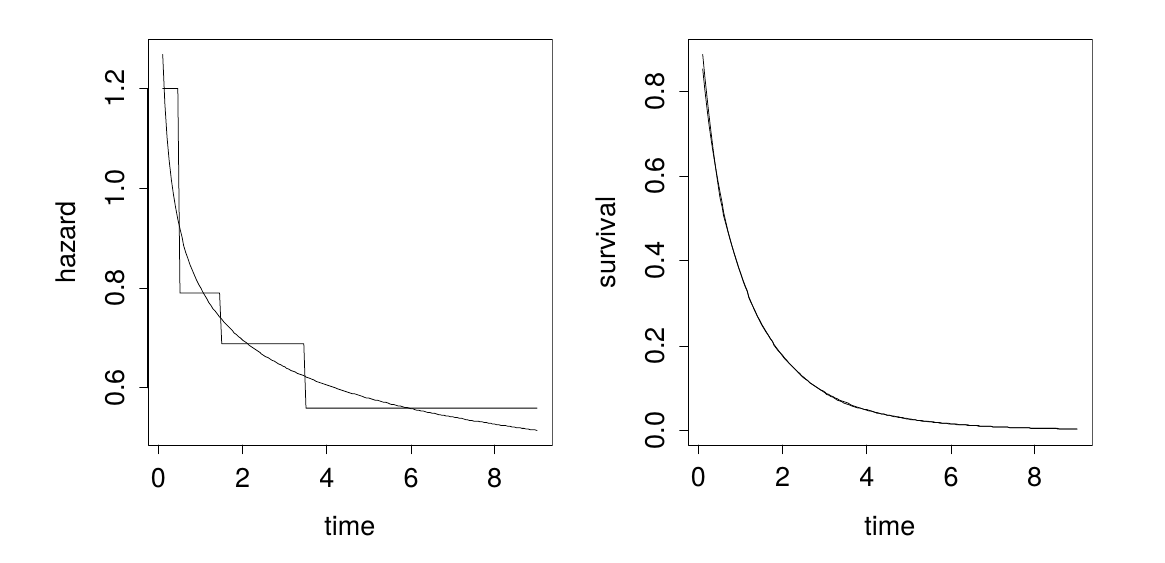
\includegraphics[height=0.2\textheight]{art/piecewise_exponential}
\caption{Piecewise Exponential aproximation of the Weibull distribution.}
\label{fig:piecewise_exponential}
\end{figure}


The piecewise-constant hazard model is very convenient to analyze under the proportional hazard assumption:
\begin{align}
	\hazard{x}{t} = \hazard{x_0}{t} e^{(x-x_0)'\beta} = h_j e^{(x-x_0)'\beta}.
\end{align}
There are $p+2J$ parameters to estimate.
This can be done directly using maximum likelihood, or by casting the problem as several separate Poisson regression problem. 
This has the benefit that the problem may be immediately solved with any statistical software suite, with existing numerical solvers.
We will currently not pursue this avenue, and refer the reader to the bibliographic notes.



\section{Collecting the pieces}
In this chapter we have seen the probabilistic reliability analysis, where we assumed components' reliabilities are known. 
We then proceeded to the statistical problem of estimating reliabilities from failure data.
We now glue collect these pieces to sketch a realistic analysis workflow, which would look roughly as follows:
\begin{enumerate}
\item Estimate reliability parameters by collecting component-wise failure data. Data is collected in a lab so that you may accelerate time and rescale to realistic operating conditions.
\item Perform the probabilistic analysis of the whole system using the estimated parameters.
\end{enumerate}


\begin{remark}[Interplay between probability and statistics]
There is obviously an interplay between the above stages:
In the statistical analysis, we want the least possible set of assumptions;
For the probabilistic analysis, the more we can assume, the more we can say about the system as a whole.
\end{remark}



\begin{remark}[What is a component?]
The notion of a ``system'' and a ``component'' is not well defined.
Indeed, for some purposes you may consider a system, as a component in a larger system.
For the statistical problem, a component is probably the smallest unit you can collect data on. At times, the smallest unit, may be the system as a whole.
\end{remark}




\section{Repairable systems}
In this section we return the a probabilistic analysis.
Unlike the previous sections, we now study systems which may be repaired after they fail.
We will thus want to study the state of the system at time $t$.
This state may depend on the number of failures and repairs performed on the system up to $t$.

We start with the introduction of some quantities of interest.
\begin{definition}[Point availability]
The point availability at time $t$, denoted $A(t)$ is defined as 
\begin{align}
	A(t):= \expect{\Phi_t}=P(\Phi_t=1) .
\end{align}
\end{definition}

\begin{definition}[Interval reliability]
When considering the availability in some time interval $J$, and denoting by $N_J$ the number of system failures in the interval, we may study
\begin{align}
	P(N_j\leq k) &\\
	M(J) &:= \expect{N_j} \\
	A(J) &:= P(\Phi_t=1), \forall t \in J.
\end{align}
\end{definition}


\begin{definition}[Interval downtime]
Denoting by $Y_J=\int_J (1-\Phi_t) dt$ the downtime during interval $J$, we may study
\begin{align}
	P(Y_j \leq y) &	\\
	A^D := \frac{\expect{Y_J}}{|J|}
\end{align}
\end{definition}

\paragraph{Limiting measures} The particular time $t$, or interval $J$ are usually not of real importance in the sense that all times and intervals are equally important.
We will thus typically be interested in the above performance measures for in some \emph{steady state} of the systems, so that the measure is representative of all $t$ (or $J$), and thus no longer depends on $t$ (or $J$).
The typical approach for this is to study the limit of the performance measure, which implies the system has reached it's steady state. Formally, this means studying $\lim_{t \to \infty}$ of the above measures. 


We now start with the analysis of a \emph{single component} system, which we later complicate into \emph{multiple component systems}. 
The required theory is that of stochastic processes, in particular \emph{counting processes}. 
The reader is referred to the bibliographic notes for rigorous proofs and details. 

\subsection{Single component systems}
For a single component, $\Phi_t=\x(t)$. 
If the component fails, it is replaced or repaired. 
We denote by $T_k$ and $R_k$ and the (random) time of the $k$'th run, and repair, respectively.
We assume $T_k \sim F$ and $R_k \sim G$, independent.

\begin{definition}[MTTF]
We denote by $\mu_F=\expect{T_k}$, the \emph{mean time to failure} (MTTF).
\end{definition}


\begin{definition}[MTTR]
We denote by $\mu_G=\expect{R_k}$, the \emph{mean time to repair} (MTTR).
\end{definition}

Obviously, MTTR and MTTF are important characteristics of the single-component system.

We denote the time to the $n$'th failure by 
\begin{align}
	S_n:= T_1 + \sum_{k=1}^{n-1} (R_k+T_{k+1})
\end{align}
where $S_0=0$ by convention.
We also denote the time to the $n$'th repair by 
\begin{align}
	S^\circ_n:= \sum_{k=1}^{n} (T_k+R_k)
\end{align}

Denoting by $H^{(n)}$ the distribution of $S_n$ we have that 
\begin{align}
	H^{(n)}(t)= F \conv (F \conv G)^{\conv (n-1)}
\end{align}
Similarly
\begin{align}
	H^{\circ(n)}(t)= (F \conv G)^{\conv (n)}
\end{align}

\begin{theorem}[Stable point availability]
As $t \to \infty$
\begin{align}
	A(t) \to \frac{\mu_F}{\mu_F+\mu_G}.
\end{align}
\end{theorem}

\begin{theorem}[Stable failures per unit of time]

As $t \to \infty$, then with probability one
\begin{align}
	\frac{N_t}{t} \to \frac{1}{\mu_F+\mu_g}
\end{align}
\end{theorem}

\begin{theorem}[Limiting unavailability]
As $t \to \infty$, then with probability one
\begin{align}
	\frac{Y_t}{t} \to 1-\frac{\mu_F}{\mu_F+\mu_G} 
\end{align}
	
\end{theorem}








\subsection{Multiple component systems}
We will now want to study the availability of a system of multiple repairable components.
The performance of the single-component system still apply, but the analysis now has to account for the fact that the state of the systems depends on the state of $n$ repairable components, assumingly independent.
By indexing the components with $i$, we denote $T_{i,k}, R_{i,k}$ for the uptime and repair time of the $k$'th failure of the $i$'th component. Their distributions are $F_i$ and $G_i$ respectively.
The system failures up to time $t$ is still $N(t)$, but not we also allow for component-wise processes $N_i(t)$, with expectations $M(t)$, and $M_i(t)$.

Denoting $A_i(t)$ the availability of component $i$ at time $t$, $A(t)$ the n-vector of reliabilities, and $A_\Phi(t)$ the whole system's reliability. 

[TODO:Complete from  \cite[Sec.4.3]{aven_stochastic_1999}]



\section{Bibliographic Notes}
An light introductory discussion, may be found in \cite{nahmias_production_2015}. 
The probabilistic analysis in this text is adapted from \cite{aven_stochastic_1999}.
The seminal reference probably being \cite{barlow_mathematical_1965}.
The statistical analysis is adapted from German Rodriguez's Generalized-Linear-Models class notes\footnote{\url{http://data.princeton.edu/wws509/notes/c7.pdf}.} and \cite[Ch.8]{natrella_nist/sematech_2010}.
For more on the statistical analysis, see \cite{cox_analysis_1984}, \cite{kalbfleisch_statistical_2002}, or \cite{klein_survival_2005}.


% 




\chapter{Revisiting System Capability Analysis}
\label{sec:advanced_capability_analysis}
[TODO]
% sec 8.4 in montgomry
\section{System Capability with Control Charts}
\section{System Capability with Designed Experiments}




% % % % % % Appendices % % % % % %
\newpage

\appendix


% % % % % % Notation % % % % %


\chapter{Notation}
\label{apx:notation}

In this text we use the following notation conventions:
\begin{description}
\item[$x$] A column vector, or scalar, as implied by the text. 
\item[$:=$] An assignment, or definition. $A:=a$ means that $A$ is defined to be $a$. 
\item[$\prod_{i=1}^{n}$] The product operator: $\prod_{i=1}^{n} x_i:= x_1 \times \dots \times x_n$
\item[$\coprod_{i=1}^{n}$] The coproduct operator: $\coprod_{i=1}^{n} x_i:= 1-(1-x_1) \times \dots \times (1-x_n)$
\item[$\#\set{A}$] The count operator. Returns the number of elements of the set $A$. Also known as the \emph{cardinality}.
\item[$\Phi(t)$] The standard Gaussian CDF at $t$: $\Phi(t):= P(Z<t)$.
\item[$\phi(t)$] The standard Gaussian density at $t$: $\phi(t):= \frac{\partial}{\partial t}\Phi(t)$.
\item[$x'$] We use $'$ for the transpose operation. For a $1\times p$ vector $x$, then $x'$ is $p \times 1$.
\item[$\x_n \rightsquigarrow \dist$] Convergence in distribution: for large enough $n$, then $\x_n$ is distributed like $\dist$.
\end{description}





% % % % % % R 


\chapter{R}
\label{apx:r}

Here is a list of packages worth knowing for SPC in \R.
The list is taken from \cite{qiu_introduction_2013}. 

\begin{description}
\item [cpm] [TODO]
\item [mnspc] [TODO]
\item [msqc] [TODO]
\item [qcc] [TODO]
\item [spc] [TODO]
\end{description}

For DOE with \R, see \url{https://cran.r-project.org/web/views/ExperimentalDesign.html}.




%%%%%%%%% Bibliography %%%%%%%%%%%
\newpage
\addcontentsline{toc}{chapter}{Bibliography}
\bibliographystyle{abbrvnat_JR}
\bibliography{QualityEngineering}
%\bibliography{quality_clean}
\label{sec:bibliography}


\end{document}